\documentclass[11pt]{book}
\usepackage[utf8x]{inputenc}
\usepackage{listings}
\usepackage{hyperref}
\usepackage{exercise}

\usepackage{algorithm}
\usepackage{algorithmicx}
\usepackage[noend]{algpseudocode}

\usepackage[toc,page]{appendix}

\usepackage[secthm,mdthm]{evan}

\usepackage{answers}

\lhead{Samuel Hsiang}

\usepackage{graphicx}

\usepackage{color}

\definecolor{myseagreen}{RGB}{88,197,191}
\definecolor{mysalmon}{RGB}{255,160,122}
\definecolor{myred}{RGB}{255,102,102}
\definecolor{mypurple}{RGB}{225,145,255}
\definecolor{myblack}{RGB}{0,0,0}
\definecolor{mywhite}{RGB}{255,255,255}

\usepackage{tikz}

\usetikzlibrary{calc,shapes.multipart,chains,arrows,positioning}

\tikzstyle{vertex}=[draw,fill=myseagreen,circle,minimum size=24pt,inner sep=0pt]

\tikzstyle{splitvertex}=[draw,fill=myseagreen,circle split,minimum size=24pt]

\usetikzlibrary{
  shapes.multipart,
  matrix,
  positioning,
  shapes.callouts,
  shapes.arrows,
  shapes.geometric,
  decorations.shapes,
  shapes,
  fit,
  arrows,
  positioning,
  trees,
  mindmap,
  calc}

\tikzset{
    squarecross/.style={
        draw, rectangle,minimum size=18pt, fill=myseagreen,
        inner sep=0pt, text=black,
        path picture = {
            \draw[black]
            (path picture bounding box.north west) -- 
            (path picture bounding box.south east)
            (path picture bounding box.south west) -- 
            (path picture bounding box.north east);
        }
    }
}

\title{Crash Course Coding Companion}
\author{Samuel Hsiang}
\date{July 2015}

\lstset{language=Java}
 
\definecolor{codegreen}{rgb}{0,0.6,0}
\definecolor{codegray}{rgb}{0.5,0.5,0.5}
\definecolor{codepurple}{rgb}{0.58,0,0.82}
\definecolor{backcolour}{rgb}{0.95,0.95,0.92}

\lstnewenvironment{mylstlisting}[1][]%
  {\noindent\minipage{\linewidth}\medskip 
   \lstset{
    backgroundcolor=\color{backcolour},   
    commentstyle=\color{codegreen},
    keywordstyle=\color{magenta},
    numberstyle=\tiny\color{codegray},
    stringstyle=\color{codepurple},
    basicstyle=\footnotesize,
    breakatwhitespace=false,         
    breaklines=true,                 
    captionpos=t,                    
    keepspaces=true,                 
    numbers=left,                    
    numbersep=5pt,                  
    showspaces=false,                
    showstringspaces=false,
    showtabs=false,                  
    tabsize=4,
   basicstyle=\ttfamily\footnotesize,
   frame=single,#1}}
  {\endminipage}

\newcommand\intro[1]{
 \section*{#1}
 \markboth{\MakeUppercase{#1}}{}
 \addcontentsline{toc}{chapter}{#1}
}

\begin{document}

\maketitle

\thispagestyle{empty}
\par\vspace*{.35\textheight}{\centering For Rachel \par}

\tableofcontents

\eject

\intro{Acknowledgements}

I am truly thankful for all my school teachers and USACO instructors, who gave me the knowledge which I wish to pass on through this text. I am grateful for Shankar and Ross, Evan, and Dr. Osborne, who separately made me believe such a task was possible. I must credit Valerie, for she was the one who drove me to really dive into and come to love computer science. Alex and Shwetark were extremely helpful with writing this text, as they provided input and helped me find problems to supplement my work. Finally, I'd like to thank all my friends and avid programmers in the TJ community. This is for all of you, and I hope you find it useful in your studies.

\intro{Preface}

You might have heard of \href{https://www.dropbox.com/s/z8qdndxmrmxqsam/Napkin.pdf?oref=e&n=97419869}{Evan Chen's Napkin}, a resource for olympiad math people that serves as a jumping point into higher mathematics.\footnote{In fact, I'm using Evan's template right now. Thanks Evan!} The Wikipedia articles on higher mathematics are just so dense in vocabulary and deter many smart young students from learning them before they are formally taught in a course in college. Evan's Napkin aims to provide that background necessary to leap right in.

I feel the same way about computer science. For most, the ease of the AP Computer Science test means that the AP coursework is often inadequate in teaching the simplest data structures, algorithms, and big ideas necessary to approach even silver USACO problems. On the other hand, even the best reference books, like Sedgewick, are too dense and unapproachable for someone who just wants to sit down and learn something interesting.\footnote{Sedgewick, notably, is getting better. \href{http://algs4.cs.princeton.edu/home/}{Check out his online companion} to \textit{Algorithms, 4th Edition}.} The road, for many, stalls here until college. Everyone should be able to learn the simplest data structures in Java or C++ standard libraries, and someone with problem-solving experience can easily jump right into understanding algorithms and more advanced data structures.

A few important notes, before we begin.

\begin{itemize}

\item

I'm assuming some fluency in C-style syntax. If this is your first time seeing code, please look somewhere else for now.

\item

It is essential that you understand the motivations and the complexities behind everything we cover. I feel that this is not stressed at all in AP Computer Science and lost under the heavy details of rigorous published works. I'm avoiding what I call the heavy details because they don't focus on the math behind the computer science and lose the bigger picture. My goal is for every mathematician or programmer, after working through this, to be able to code short scripts to solve problems. Once you understand how things work, you can then move on to those details which are necessary for building larger projects. The heavy details become meaningless as languages develop or become phased out. The math and ideas behind the data structures and algorithms will last a lifetime.

\item

It is recommended actually code up each data structure with its most important functions or algorithm as you learn them. I truly believe the only way to build a solid foundation is to code. Do not become reliant on using the standard library (\texttt{java.util}, for instance) without understanding how the tool you are using works.

\end{itemize}

\chapter{Fundamentals}

\section{Comparable}

The interface \texttt{Comparable} is how Java can impose an ordering on any object. Implementing \texttt{Comparable} requires support to the method \texttt{int compareTo(Object o)}. If \texttt{a.compareTo(b) < 0}, then \texttt{a} should come before \texttt{b} in the ordering. If \texttt{a.compareTo(b) > 0}, then \texttt{a} should come after \texttt{b} in the ordering. If \texttt{a.compareTo(b)==0}, then \texttt{a} is considered to be equal to \texttt{b}. \texttt{a.compareTo(b) == 0} should be equivalent to \texttt{a.equals(b)}. For example, consider the following \texttt{class MyPair}:

\begin{mylstlisting}
class MyPair implements Comparable {
	int x;
	int y;
    // sort by x-coordinate first
	public int compareTo(Object o) {
		MyPair c = (MyPair) o;
		if(x < c.x) return -1;
		if(x > c.x) return 1;
		// if x-coordinates equal, compare y
		if(y < c.x) return -1;
		if(y > c.x) return 1;
		return 0; // equal
	}
}
\end{mylstlisting}

We can also clean this up a bit using generics:

\begin{mylstlisting}
class MyPair implements Comparable<MyPair> {
	int x;
	int y;
	public int compareTo(MyPair c) {
		if(x < c.x) return -1;
		if(x > c.x) return 1;
		if(y < c.x) return -1;
		if(y > c.x) return 1;
		return 0;
	}
}
\end{mylstlisting}

Note that no casting is required anymore.

\section{Sorts}

\subsection{Merge Sort}

The idea behind merge sort is simple. If we are given two equally sized sorted stacks, we could easily combine them into one sorted stack by comparing the top of the two stacks only, since the smallest element remaining must be one of those two.

From here, we divide and conquer. Simply cut the array in half, recurse on each half, and merge the two back together. This runs in $O(n \log (n))$ time.

\subsection{Quicksort}

Quicksort also uses a divide and conquer strategy to achieve an $O(n \log (n))$ amortized bound. We take a random element from the array, move anything less than it to the left of the array, anything right of it to the right of the array, and recurse.

This was previously implemented by \texttt{Arrays.sort()} and \texttt{Collections.sort()}, but Java now uses either dual-pivot quicksort or timsort.

\section{Binary Search}

Before we begin studying data structures, it is necessary to first understand general search techniques. Given a list, it is straightforward to simply check every element in the list in a linear search.

One way we can make this faster is by imposing an ordering on the list. Then inserting elements becomes slower because we can no longer just pop the element to the the end of the list. However, if we are asked to find an element, we know roughly where in the list to search because we can compare the element to other elements in the list.

Consider an array of sorted elements. The array supports $O(1)$ access to any element in the array. We'll take a look at the middle element in the array. Depending on whether or not the element to be searched is larger, smaller, or equal to the middle element, we can guarantee we can eliminate half of the array. Then finding an element is an $O(\log{n})$ operation on a sorted array. This can be done either iteratively or recursively.

\chapter{Java Standard Library Data Structures}

The purpose of this chapter is to provide an overview on how the most basic and useful data structures work. The implementations of most higher-level languages already coded these for us, but it is important to know how each data structure works rather than blindly use the standard library.

More technical explanations of all of these can be found, mostly under the package \texttt{java.util}, in the \href{https://docs.oracle.com/javase/8/docs/api/}{Java API}.

I strongly believe that Java is better than C++ for beginning programmers. It forces people into good coding habits, and though the lack of pointers initially frustrated me, it really does make learning general concepts liked LinkedLists much easier, as the intricacies of the C++ pointer no longer distract from the larger idea.

\section{Generics}

You may or may not have seen these used before:
\begin{verbatim}
ArrayList<Integer> al = new ArrayList<Integer>();
\end{verbatim}
This means that \texttt{al} is an ArrayList of Integers. We can only add Integers into the ArrayList, and anything removed from the ArrayList is guaranteed to be an Integer. I don't think the beginning programmer needs to know how to necessarily code a class that supports generics. However, you are going to use the standard library, so you should know how to use a class that does support generics. I think standard classes are relatively straightforward to use but can be annoying to actually implement.

\textbf{For simplicity, all data structures will store Strings.}

\section{List}

A List is a collection of objects with an ordering. Users of a list have control over where in the list each object is and can access a specific element by its index, like in an array.

\subsection{ArrayList}

What is nice about an array? We can access or change any element we want in the array in $O(1)$ time. The problem is that an array has fixed length. It's not easy to append an element to the end of an array.

The fix to this is pretty simple. Why not just make a bigger array, and copy everything over to the new array? Then there's more room at the end to add a new element. This is the idea behind an ArrayList. If the backbone array runs out of space, we create a new array with double the size and keep going as if nothing happened.

\begin{center}
{
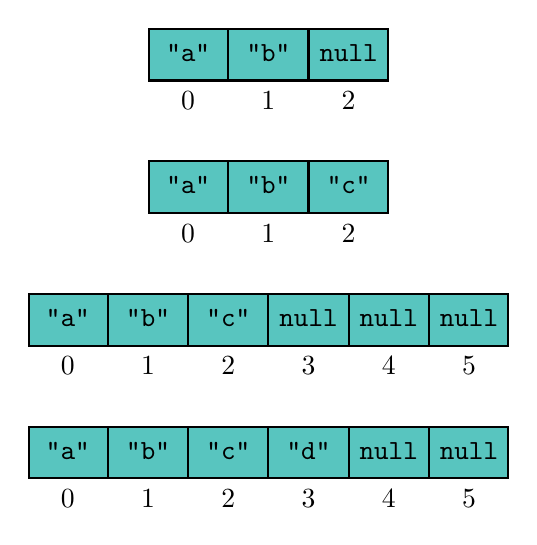
\begin{tikzpicture}[
  thick,
  myrect/.style={
    draw,
    fill=myseagreen,
    rectangle split,
    rectangle split horizontal,
    rectangle split parts=#1,
    rectangle split part align=left,
    text width=5ex,
    text centered
    },
  mycallout/.style={
    shape=rectangle callout,
    rounded corners,
    fill=mysalmon,
    callout absolute pointer={#1},
    callout pointer width=1cm
  }  
]

\node[myrect=3]
  (array1)
  {
  					\strut \texttt{"a"}
  \nodepart{two}	\strut \texttt{"b"}
  \nodepart{three}	\strut \texttt{null}
  };
\foreach \Valor [count=\Valori from 0] in {one ,two ,three }
  \node[below] at (array1.\Valor south) {\Valori};

\node[myrect=3]
  (array2)[below=of array1]
  {
  					\strut \texttt{"a"}
  \nodepart{two}	\strut \texttt{"b"}
  \nodepart{three}	\strut \texttt{"c"}
  };
\foreach \Valor [count=\Valori from 0] in {one ,two ,three }
  \node[below] at (array2.\Valor south) {\Valori};

\node[myrect=6]
  (array3)[below=of array2]
  {
  					\strut \texttt{"a"}
  \nodepart{two}	\strut \texttt{"b"}
  \nodepart{three}	\strut \texttt{"c"}
  \nodepart{four}	\strut \texttt{null}
  \nodepart{five}	\strut \texttt{null}
  \nodepart{six}	\strut \texttt{null}
  };
\foreach \Valor [count=\Valori from 0] in {one ,two ,three , four , five , six }
  \node[below] at (array3.\Valor south) {\Valori};

\node[myrect=6]
  (array4)[below=of array3]
  {
  					\strut \texttt{"a"}
  \nodepart{two}	\strut \texttt{"b"}
  \nodepart{three}	\strut \texttt{"c"}
  \nodepart{four}	\strut \texttt{"d"}
  \nodepart{five}	\strut \texttt{null}
  \nodepart{six}	\strut \texttt{null}
  };
\foreach \Valor [count=\Valori from 0] in {one ,two ,three , four , five , six }
  \node[below] at (array4.\Valor south) {\Valori};

\end{tikzpicture}
}
\end{center}

We see that there is still room in the array to add \texttt{"c"}, but to add more elements to the list, we must use a new array with double the length.

It's important to note that any given insertion to the ArrayList is either $O(n)$ or $O(1)$, but there is only one $O(n)$ insertion for every $O(n)$ $O(1)$ insertions, so we still average out to constant time.

\begin{itemize}

\item
\texttt{boolean add(String s)} -- add an element to the end of the list. (By convention, this returns \texttt{true} if the addition was successful, and \texttt{false} otherwise.)
\item
\texttt{void add(int i, String s)} -- shift everything from position \texttt{i} onward down by one, and add \texttt{s} at position \texttt{i}.
\item
\texttt{boolean contains(Object o)} -- return \texttt{true} if \texttt{o} is stored in the ArrayList, and \texttt{false} otherwise. Remember to cast \texttt{o} to a String.
\item
\texttt{String get(int i)} -- return the element stored at index \texttt{i}.
\item
\texttt{boolean isEmpty()} -- return \texttt{true} if \texttt{size() == 0}.
\item
\texttt{String remove(int i)} -- remove and return the element at index $i$ from the list. (Why is this annoying?)
\item
\texttt{String set(int i, String s)} -- replace the element stored at index \texttt{i} with \texttt{s}, and return the element that was originally at position \texttt{i}.
\item
\texttt{int size()} -- note that this is not just the length of the backbone array.
\end{itemize}

The \texttt{get} and \texttt{set} functions are very nice. They are easy to code and run in constant time. These are the bread and butter of any array. Adding at the end of the ArrayList is nice as well. \texttt{contains} is a pain, as it is $O(n)$, and adding to and removing from early in the list are more annoying.

If this is your first time seeing an ArrayList, I would suggest coding up your own. It should be relatively straightforward.

\subsection{LinkedList}

Arrays are nice for accessing, say, the seventh element in the list. We extend this to an ArrayList to implement adding and removing elements to and from the end of the list nicely. Removing elements from the beginning of the list, however, is cumbersome.

The LinkedList attempts to remedy this. It trades $O(1)$ access to any element in the list for an easier way to remove elements from either end of the list easily. Consider a chain of paper clips:

\begin{center}

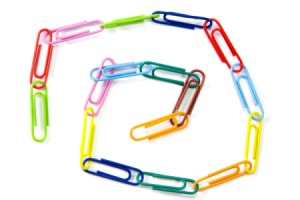
\includegraphics{paper_clip_chain.jpg}

\end{center}

It's easy to add or remove more paper clips from either end of the chain, and from any given paper clip, it's easy to access the paper clip directly previous or next to it in the chain. If we needed the seventh paper clip in the chain, we'd need to manually count, an $O(n)$ operation. However, if we then needed to remove that paper clip from the chain, it wouldn't be that hard, assuming we kept a finger on the seventh paper clip.

The standard library implements a cyclical doubly-linked list, with a dummy head. It looks something like this:

\begin{center}


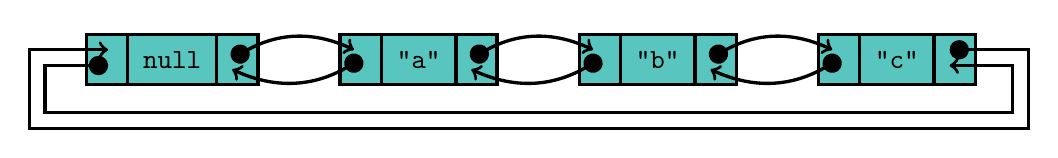
\begin{tikzpicture}[
        list/.style={
            very thick, rectangle split, 
            rectangle split parts=3, draw, 
            rectangle split horizontal, minimum size=18pt,
            inner sep=5pt, text=black,
            rectangle split part fill=myseagreen
        }, 
        ->, start chain, very thick
      ]

  \node[list,on chain] (dummy) {\nodepart{second} \texttt{null}};
  \node[list,on chain] (A) {\nodepart{second} \texttt{"a"}};
  \node[list,on chain] (B) {\nodepart{second} \texttt{"b"}};
  \node[list,on chain] (C) {\nodepart{second} \texttt{"c"}};

    \path[*->] let \p1 = (dummy.three), \p2 = (dummy.center) in (\x1,\y2) edge [bend left] ($(A.one)+(0,0.2)$);
  \path[*->] let \p1 = (A.three), \p2 = (A.center) in (\x1,\y2) edge [bend left] ($(B.one)+(0,0.2)$);
  \path[*->] let \p1 = (B.three), \p2 = (B.center) in (\x1,\y2) edge [bend left] ($(C.one)+(0,0.2)$);
  
%  \draw[*->] let \p1 = (C.three), \p2 = (C.center) in (\x1,\y2) -- (dummy);

%  \draw[*->] ($(A.one)+(0.2,0.1)$) -- (dummy);
  \path[*->] ($(B.one)+(0.1,0.1)$) edge [bend left] ($(A.three)+(0,-0.05)$);
  \path[*->] ($(C.one)+(0.1,0.1)$) edge [bend left] ($(B.three)+(0,-0.05)$);
    \path[*->] ($(A.one)+(0.1,0.1)$) edge [bend left] ($(dummy.three)+(0,-0.05)$);
    
    \draw[*->] ($(C.three)+(0.0,0.2)$) -- ($(C.three)+(1.0,0.2)$) -- ($(C.three)+(1.0,-0.8)$) -- ($(dummy.one)+(-0.9,-0.8)$) -- ($(dummy.one)+(-0.9,0.2)$) -- ($(dummy.one)+(0.1,0.2)$);

    \draw[<-*] ($(C.three)+(0.0,0.0)$) -- ($(C.three)+(0.8,0.0)$) -- ($(C.three)+(0.8,-0.6)$) -- ($(dummy.one)+(-0.7,-0.6)$) -- ($(dummy.one)+(-0.7,0.0)$) -- ($(dummy.one)+(0.1,0.0)$);

\end{tikzpicture}

\end{center}

We see that each node maintains a pointer to its next neighbor and its previous neighbor, in addition to containing the String it stores. We can store this data in a class like the following:

\begin{mylstlisting}
class ListNode {
	ListNode prev, next;
    String s;
}
\end{mylstlisting}

If we were to insert an element after a ListNode \texttt{a}, it is necessary to update all pointers:

\begin{mylstlisting}
ListNode b = new ListNode();
b.prev = a;
b.next = a.next;
b.next.prev = b;
a.next = b;
\end{mylstlisting}

Since the LinkedList is symmetric, inserting an element before a node is also easy. To add something to the end of the list, simply add it before the dummy head. From here it should not be too hard to implement all the important functions of a LinkedList.

\begin{itemize}

\item \texttt{boolean add(String s)} -- add to the end.
\item \texttt{void add(int i, String s)} -- this is linear. Don't forget about 0-indexing.
\item \texttt{void addFirst()}
\item \texttt{boolean contains(Object o)}
\item \texttt{String get(int i)}
\item \texttt{String getFirst()}
\item \texttt{String getLast()}
\item \texttt{boolean isEmpty()}
\item \texttt{String remove()} -- remove the last element.
\item \texttt{String remove(int i)}
\item \texttt{String removeFirst()}
\item \texttt{String set(int i, String s)}
\item \texttt{int size()}

\end{itemize}

With a LinkedList implemented, two other data structures immediately follow.

\subsection{Stack}

A stack is is literally a stack. If we have a stack of papers, we can \textit{push} things on the top and \textit{pop} things off the top. Sometimes we \textit{peek} at what's on the top but don't actually remove anything. We never do anything with what's on the bottom. This is called \textit{LIFO}: Last In, First Out.

\begin{itemize}

\item \texttt{String push(String s)} -- pushes the item on the top of the stack, and returns the same element.

\item \texttt{String pop()} -- removes the item at the top of the stack and returns it.

\item \texttt{String peek()} -- returns the top element but does not remove it.

\end{itemize}

Java implements a Stack using an ArrayList-like structure. This works just as well, and is faster in practice, but I prefer the LinkedList structure as a mathematical concept as it is more elegant and more easily customizable.

\subsection{Queue}

A queue is like a lunch line. We \textit{add} things to the end and \textit{poll} things from the front. Sometimes we \textit{peek} at the front but don't actually remove anything. The first person in line gets served first. This is called \textit{FIFO}: First In, First Out.

\begin{itemize}

\item \texttt{boolean add(String s)}

\item \texttt{String poll()} -- removes the item at the front of the queue and returns it. Same thing as \texttt{remove()}.

\item \texttt{String peek()}

\end{itemize}

In Java, \texttt{Queue} is an interface. This means that we cannot instantiate a \texttt{Queue}, so the following statement is illegal.

\begin{mylstlisting}
Queue<String> q = new Queue<String>();
\end{mylstlisting}

Instead, we must do something like this:

\begin{mylstlisting}
Queue<String> q = new Queue<LinkedList>();
\end{mylstlisting}

This is legal because LinkedList implements Queue. Queue, however, does not extend List, so it is somewhat untruthful to place Queue under List in this book. However, I do want to stress that the LinkedList is the standard FIFO queue.

\section{PriorityQueue}

Quite often a FIFO queue is not always desirable. Maybe the String I want to remove at every given point is the one that is lexicographically least. a PriorityQueue is a Queue that allows us to do this using what is known as a \textit{heap}.

A min heap is a tree such that every node is smaller than or equal to all of its children. Pictured is a complete binary min heap, which will be of most use to us.

\begin{center}
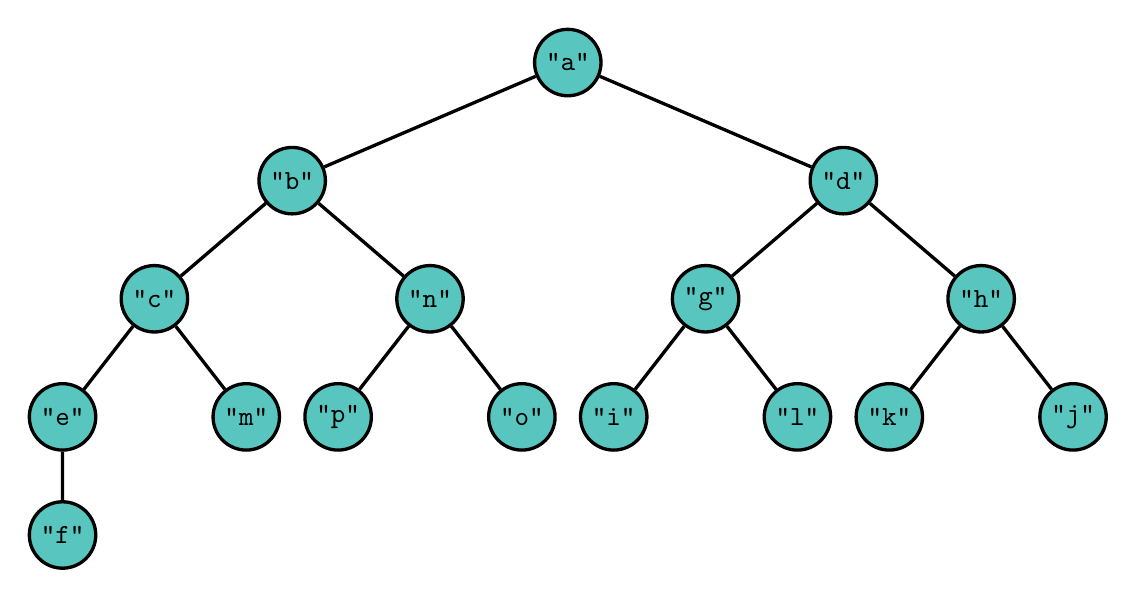
\begin{tikzpicture}[very thick,level/.style={sibling distance=70mm/#1}]
\node [vertex] (r){\texttt{"a"}}
  child {
    node [vertex] (a) {\texttt{"b"}}
    child {
      node [vertex] {\texttt{"c"}}
      child {
        node [vertex] {\texttt{"e"}}
        child {node [vertex] {\texttt{"f"}}}
      } 
      child {
        node [vertex] {\texttt{"m"}}
      }
    }
    child {
      node [vertex] {\texttt{"n"}}
      child {node [vertex] {\texttt{"p"}}}
      child {node [vertex] {\texttt{"o"}}}
    }
  }
  child {
    node [vertex] {\texttt{"d"}}
    child {
      node [vertex] {\texttt{"g"}}
      child {node [vertex] {\texttt{"i"}}}
      child {node [vertex] {\texttt{"l"}}}
    }
    child {
      node [vertex] {\texttt{"h"}}
      child {node [vertex] {\texttt{"k"}}}
      child {node [vertex] {\texttt{"j"}}}
    }
  };
\end{tikzpicture}
\end{center}

We see that the root of the tree will always be the top element. It is tempting to use a container class with a pointer to its left and its right child. However, we have a much nicer way to store \textit{complete} binary trees with an array. Consider the following numbering of the nodes:

\begin{center}
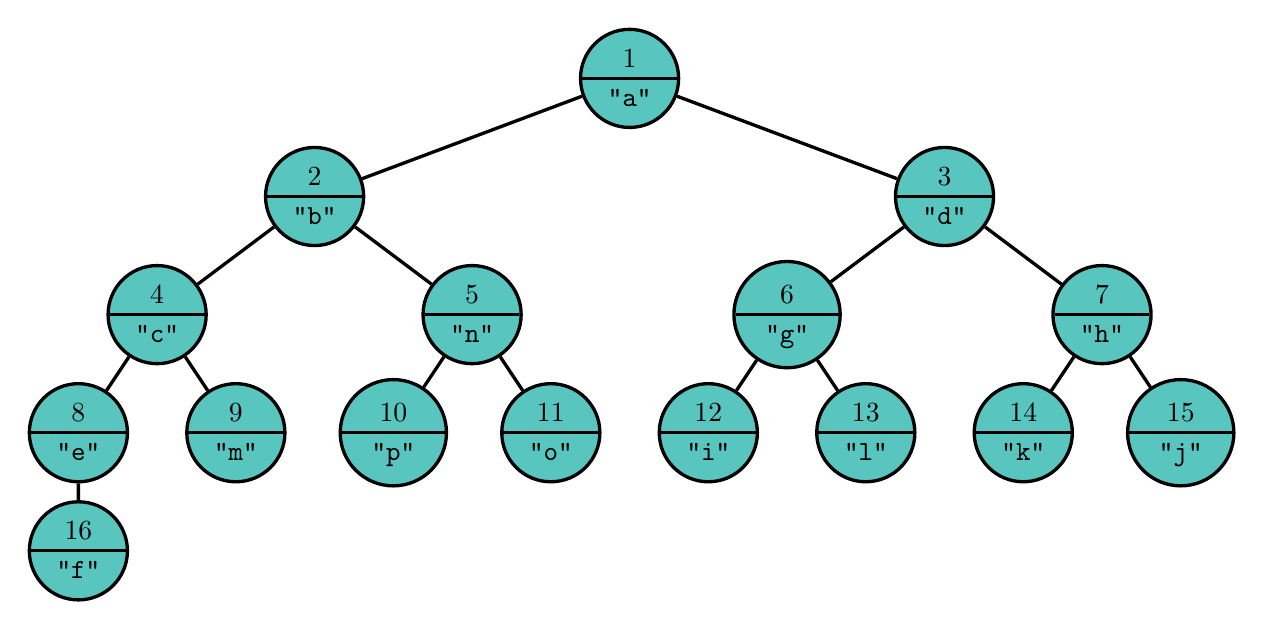
\begin{tikzpicture}[very thick,level 1/.style={sibling distance=80mm}, level 2/.style={sibling distance=40mm}, level 3/.style={sibling distance=20mm}]
\node [splitvertex] (r){1\nodepart{lower}\texttt{"a"}}
  child {
    node [splitvertex] (a) {2\nodepart{lower}\texttt{"b"}}
    child {
      node [splitvertex] {4\nodepart{lower}\texttt{"c"}}
      child {
        node [splitvertex] {8\nodepart{lower}\texttt{"e"}}
        child {node [splitvertex] {16\nodepart{lower}\texttt{"f"}}}
      } 
      child {
        node [splitvertex] {9\nodepart{lower}\texttt{"m"}}
      }
    }
    child {
      node [splitvertex] {5\nodepart{lower}\texttt{"n"}}
      child {node [splitvertex] {10\nodepart{lower}\texttt{"p"}}}
      child {node [splitvertex] {11\nodepart{lower}\texttt{"o"}}}
    }
  }
  child {
    node [splitvertex] {3\nodepart{lower}\texttt{"d"}}
    child {
      node [splitvertex] {6\nodepart{lower}\texttt{"g"}}
      child {node [splitvertex] {12\nodepart{lower}\texttt{"i"}}}
      child {node [splitvertex] {13\nodepart{lower}\texttt{"l"}}}
    }
    child {
      node [splitvertex] {7\nodepart{lower}\texttt{"h"}}
      child {node [splitvertex] {14\nodepart{lower}\texttt{"k"}}}
      child {node [splitvertex] {15\nodepart{lower}\texttt{"j"}}}
    }
  };
\end{tikzpicture}
\end{center}

We see that every number from 1 to 16 is used, and for every node, if the index associated with it is $i$, the left child is $2i$, and the right child is $2i+1$. This leads to a very natural implementation of the tree in an array:

\begin{center}
{
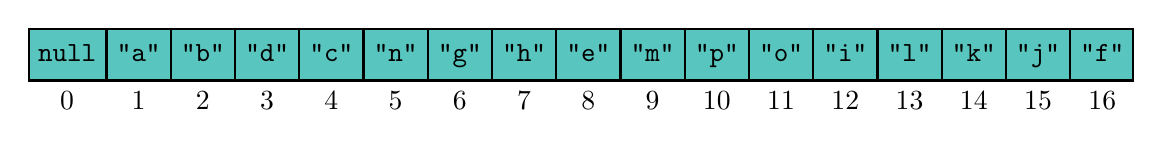
\begin{tikzpicture}[
  thick,
  myrect/.style={
    draw,
    fill=myseagreen,
    rectangle split,
    rectangle split horizontal,
    rectangle split parts=#1,
    rectangle split part align=left,
    text centered
    },
  mycallout/.style={
    shape=rectangle callout,
    rounded corners,
    fill=mysalmon,
    callout absolute pointer={#1},
    callout pointer width=1cm
  }  
]

\node[myrect=17]
  (array)
  {
  					\strut \texttt{null}
  \nodepart{two}	\strut \texttt{"a"}
  \nodepart{three}	\strut \texttt{"b"}
  \nodepart{four}	\strut \texttt{"d"}
  \nodepart{five}	\strut \texttt{"c"}
  \nodepart{six}	\strut \texttt{"n"}
  \nodepart{seven}	\strut \texttt{"g"}
  \nodepart{eight}	\strut \texttt{"h"}
  \nodepart{nine}	\strut \texttt{"e"}
  \nodepart{ten}	\strut \texttt{"m"}
  \nodepart{eleven}	\strut \texttt{"p"}
  \nodepart{twelve}	\strut \texttt{"o"}
  \nodepart{thirteen}	\strut \texttt{"i"}
  \nodepart{fourteen}	\strut \texttt{"l"}
  \nodepart{fifteen}	\strut \texttt{"k"}
  \nodepart{sixteen}	\strut \texttt{"j"}
  \nodepart{seventeen}	\strut \texttt{"f"}
  };
\foreach \Valor [count=\Valori from 0] in {one ,two ,three ,four ,five ,six ,seven ,eight ,nine ,ten ,eleven ,twelve ,thirteen ,fourteen ,fifteen ,sixteen ,seventeen }
  \node[below] at (array.\Valor south) {\Valori};

\end{tikzpicture}
}
\end{center}

How do we add elements to our heap, while maintaining the heap qualities? Well, let's just add it to the very end and see what we get. Suppose we are to add \texttt{"b"} to the tree.

\begin{center}
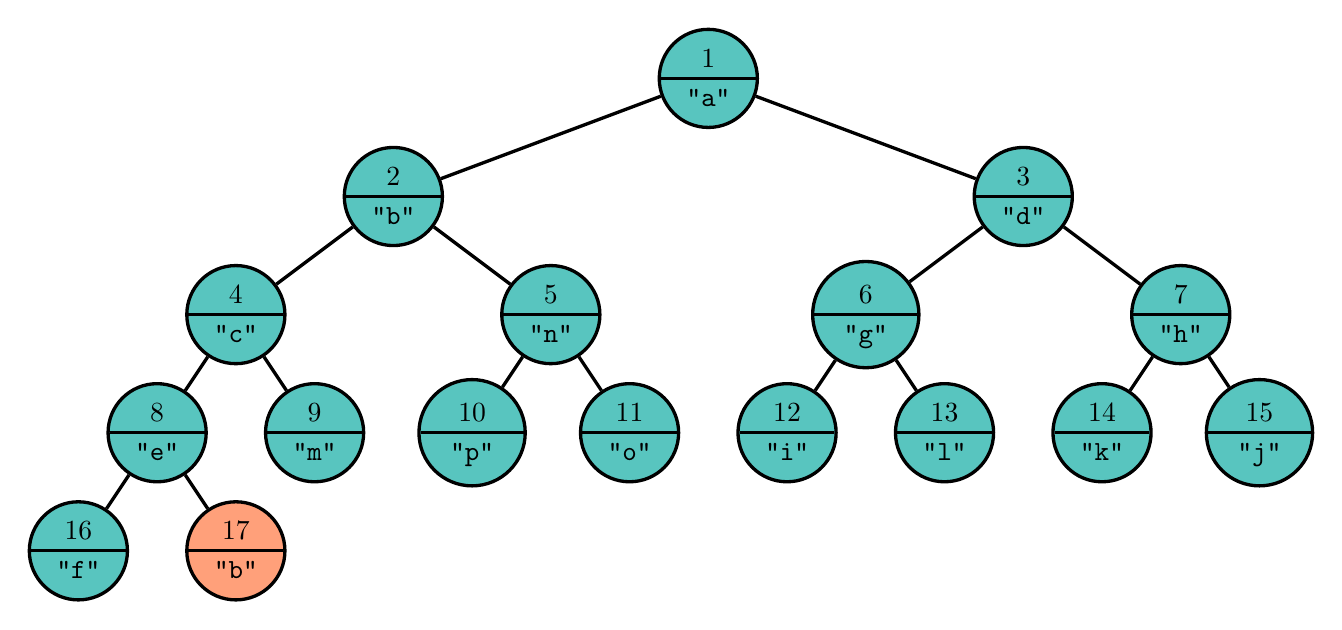
\begin{tikzpicture}[very thick,level 1/.style={sibling distance=80mm}, level 2/.style={sibling distance=40mm}, level 3/.style={sibling distance=20mm}]
\node [splitvertex] (r){1\nodepart{lower}\texttt{"a"}}
  child {
    node [splitvertex] (a) {2\nodepart{lower}\texttt{"b"}}
    child {
      node [splitvertex] {4\nodepart{lower}\texttt{"c"}}
      child {
        node [splitvertex] {8\nodepart{lower}\texttt{"e"}}
        child {node [splitvertex] {16\nodepart{lower}\texttt{"f"}}}
        child {node [splitvertex, fill=mysalmon] {17\nodepart{lower}\texttt{"b"}}}
      } 
      child {
        node [splitvertex] {9\nodepart{lower}\texttt{"m"}}
      }
    }
    child {
      node [splitvertex] {5\nodepart{lower}\texttt{"n"}}
      child {node [splitvertex] {10\nodepart{lower}\texttt{"p"}}}
      child {node [splitvertex] {11\nodepart{lower}\texttt{"o"}}}
    }
  }
  child {
    node [splitvertex] {3\nodepart{lower}\texttt{"d"}}
    child {
      node [splitvertex] {6\nodepart{lower}\texttt{"g"}}
      child {node [splitvertex] {12\nodepart{lower}\texttt{"i"}}}
      child {node [splitvertex] {13\nodepart{lower}\texttt{"l"}}}
    }
    child {
      node [splitvertex] {7\nodepart{lower}\texttt{"h"}}
      child {node [splitvertex] {14\nodepart{lower}\texttt{"k"}}}
      child {node [splitvertex] {15\nodepart{lower}\texttt{"j"}}}
    }
  };
\end{tikzpicture}
\end{center}

Well, \texttt{"b"} comes before \texttt{"e"} in the alphabet, so let's swap the nodes. We are guaranteed that \texttt{"b"} should come before the other child (in this case, \texttt{"f"}) by the transitive property.

\begin{center}
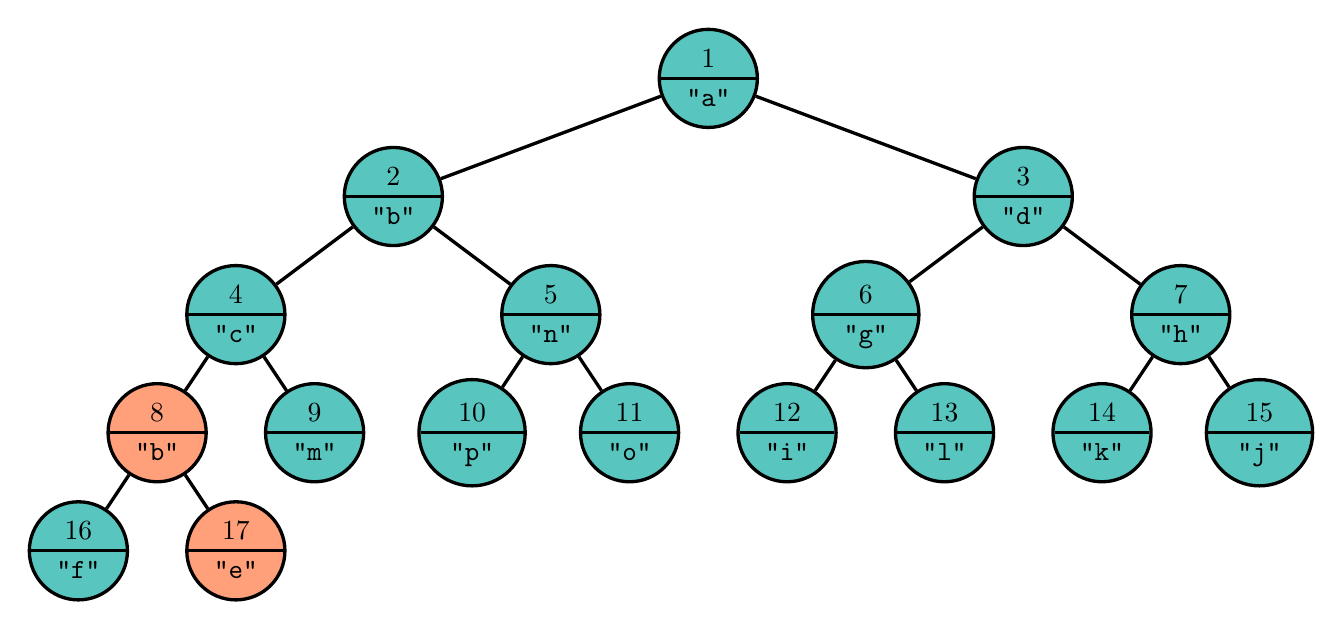
\begin{tikzpicture}[very thick,level 1/.style={sibling distance=80mm}, level 2/.style={sibling distance=40mm}, level 3/.style={sibling distance=20mm}]
\node [splitvertex] (r){1\nodepart{lower}\texttt{"a"}}
  child {
    node [splitvertex] (a) {2\nodepart{lower}\texttt{"b"}}
    child {
      node [splitvertex] {4\nodepart{lower}\texttt{"c"}}
      child {
        node [splitvertex, fill=mysalmon] {8\nodepart{lower}\texttt{"b"}}
        child {node [splitvertex] {16\nodepart{lower}\texttt{"f"}}}
        child {node [splitvertex, fill=mysalmon] {17\nodepart{lower}\texttt{"e"}}}
      } 
      child {
        node [splitvertex] {9\nodepart{lower}\texttt{"m"}}
      }
    }
    child {
      node [splitvertex] {5\nodepart{lower}\texttt{"n"}}
      child {node [splitvertex] {10\nodepart{lower}\texttt{"p"}}}
      child {node [splitvertex] {11\nodepart{lower}\texttt{"o"}}}
    }
  }
  child {
    node [splitvertex] {3\nodepart{lower}\texttt{"d"}}
    child {
      node [splitvertex] {6\nodepart{lower}\texttt{"g"}}
      child {node [splitvertex] {12\nodepart{lower}\texttt{"i"}}}
      child {node [splitvertex] {13\nodepart{lower}\texttt{"l"}}}
    }
    child {
      node [splitvertex] {7\nodepart{lower}\texttt{"h"}}
      child {node [splitvertex] {14\nodepart{lower}\texttt{"k"}}}
      child {node [splitvertex] {15\nodepart{lower}\texttt{"j"}}}
    }
  };
\end{tikzpicture}
\end{center}

One more swap...

\begin{center}
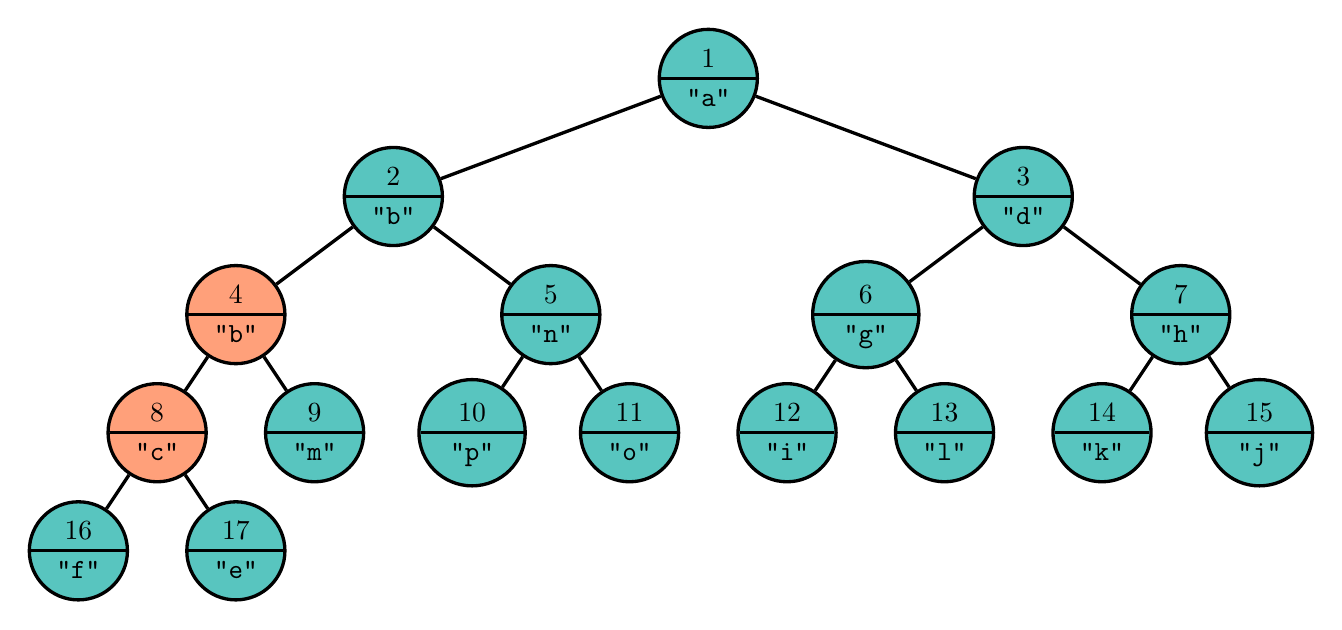
\begin{tikzpicture}[very thick,level 1/.style={sibling distance=80mm}, level 2/.style={sibling distance=40mm}, level 3/.style={sibling distance=20mm}]
\node [splitvertex] (r){1\nodepart{lower}\texttt{"a"}}
  child {
    node [splitvertex] (a) {2\nodepart{lower}\texttt{"b"}}
    child {
      node [splitvertex, fill=mysalmon] {4\nodepart{lower}\texttt{"b"}}
      child {
        node [splitvertex, fill=mysalmon] {8\nodepart{lower}\texttt{"c"}}
        child {node [splitvertex] {16\nodepart{lower}\texttt{"f"}}}
        child {node [splitvertex] {17\nodepart{lower}\texttt{"e"}}}
      } 
      child {
        node [splitvertex] {9\nodepart{lower}\texttt{"m"}}
      }
    }
    child {
      node [splitvertex] {5\nodepart{lower}\texttt{"n"}}
      child {node [splitvertex] {10\nodepart{lower}\texttt{"p"}}}
      child {node [splitvertex] {11\nodepart{lower}\texttt{"o"}}}
    }
  }
  child {
    node [splitvertex] {3\nodepart{lower}\texttt{"d"}}
    child {
      node [splitvertex] {6\nodepart{lower}\texttt{"g"}}
      child {node [splitvertex] {12\nodepart{lower}\texttt{"i"}}}
      child {node [splitvertex] {13\nodepart{lower}\texttt{"l"}}}
    }
    child {
      node [splitvertex] {7\nodepart{lower}\texttt{"h"}}
      child {node [splitvertex] {14\nodepart{lower}\texttt{"k"}}}
      child {node [splitvertex] {15\nodepart{lower}\texttt{"j"}}}
    }
  };
\end{tikzpicture}
\end{center}

And now we have the heap property restored. As the tree has depth at most $\log{n}$, this process is $O(\log{n})$.

To remove the root from the heap, we replace the root with the last leaf:

\begin{center}
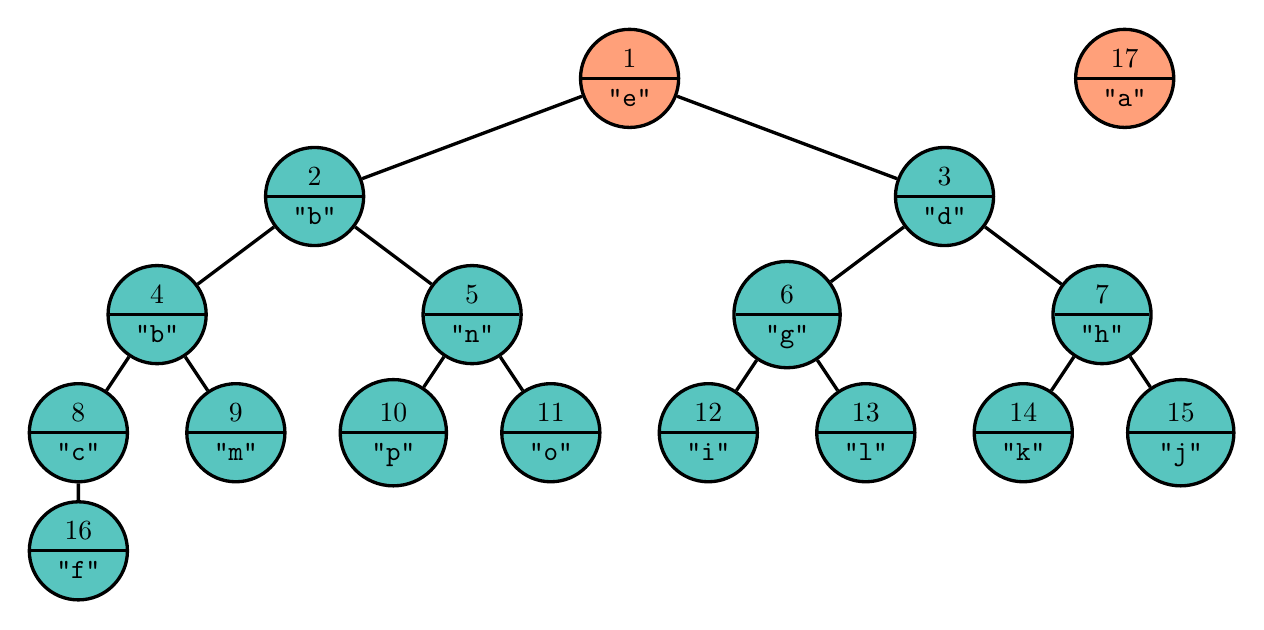
\begin{tikzpicture}[very thick,level 1/.style={sibling distance=80mm}, level 2/.style={sibling distance=40mm}, level 3/.style={sibling distance=20mm}]
\node [splitvertex, fill=mysalmon] (r){1\nodepart{lower}\texttt{"e"}}
  child {
    node [splitvertex] (a) {2\nodepart{lower}\texttt{"b"}}
    child {
      node [splitvertex] {4\nodepart{lower}\texttt{"b"}}
      child {
        node [splitvertex] {8\nodepart{lower}\texttt{"c"}}
        child {node [splitvertex] {16\nodepart{lower}\texttt{"f"}}}
      } 
      child {
        node [splitvertex] {9\nodepart{lower}\texttt{"m"}}
      }
    }
    child {
      node [splitvertex] {5\nodepart{lower}\texttt{"n"}}
      child {node [splitvertex] {10\nodepart{lower}\texttt{"p"}}}
      child {node [splitvertex] {11\nodepart{lower}\texttt{"o"}}}
    }
  }
  child {
    node [splitvertex] {3\nodepart{lower}\texttt{"d"}}
    child {
      node [splitvertex] {6\nodepart{lower}\texttt{"g"}}
      child {node [splitvertex] {12\nodepart{lower}\texttt{"i"}}}
      child {node [splitvertex] {13\nodepart{lower}\texttt{"l"}}}
    }
    child {
      node [splitvertex] {7\nodepart{lower}\texttt{"h"}}
      child {node [splitvertex] {14\nodepart{lower}\texttt{"k"}}}
      child {node [splitvertex] {15\nodepart{lower}\texttt{"j"}}}
    }
  };
  \node [splitvertex, fill=mysalmon] [right=5cm of r]{17\nodepart{lower}\texttt{"a"}};
\end{tikzpicture}
\end{center}

We perform a series of swaps to restore the heap property. We always want to choose the smaller child to swap until the heap property is satisfied.

\begin{center}
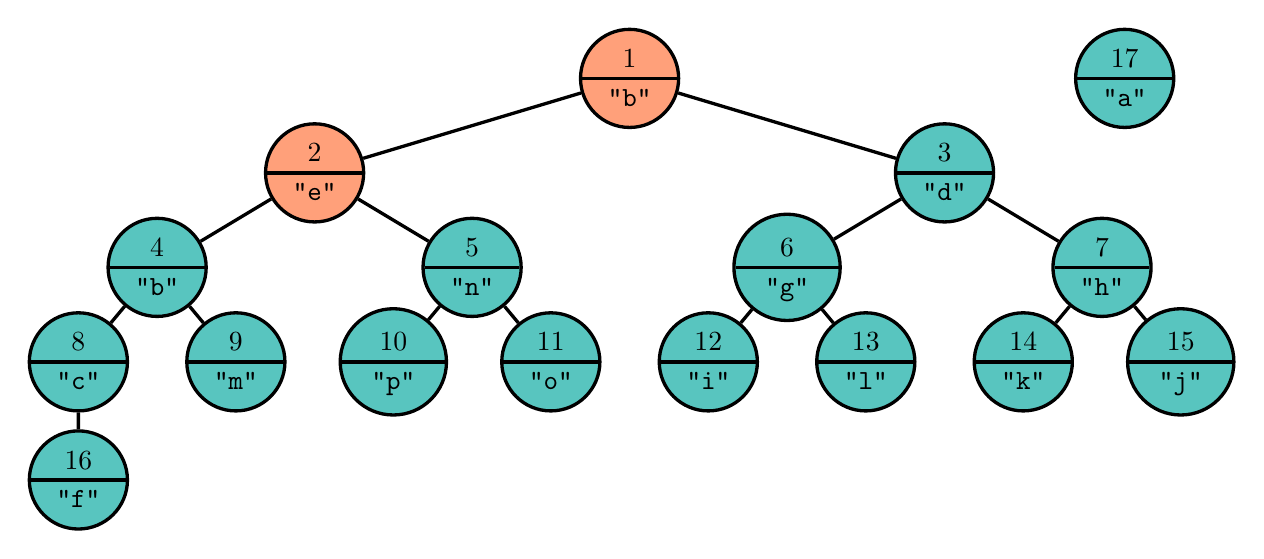
\begin{tikzpicture}[very thick,level 1/.style={sibling distance=80mm}, level 2/.style={sibling distance=40mm}, level 3/.style={sibling distance=20mm}, level distance=12mm, level 4/.style={level distance=15mm}]
\node [splitvertex, fill=mysalmon] (r){1\nodepart{lower}\texttt{"b"}}
  child {
    node [splitvertex, fill=mysalmon] (a) {2\nodepart{lower}\texttt{"e"}}
    child {
      node [splitvertex] {4\nodepart{lower}\texttt{"b"}}
      child {
        node [splitvertex] {8\nodepart{lower}\texttt{"c"}}
        child {node [splitvertex] {16\nodepart{lower}\texttt{"f"}}}
      } 
      child {
        node [splitvertex] {9\nodepart{lower}\texttt{"m"}}
      }
    }
    child {
      node [splitvertex] {5\nodepart{lower}\texttt{"n"}}
      child {node [splitvertex] {10\nodepart{lower}\texttt{"p"}}}
      child {node [splitvertex] {11\nodepart{lower}\texttt{"o"}}}
    }
  }
  child {
    node [splitvertex] {3\nodepart{lower}\texttt{"d"}}
    child {
      node [splitvertex] {6\nodepart{lower}\texttt{"g"}}
      child {node [splitvertex] {12\nodepart{lower}\texttt{"i"}}}
      child {node [splitvertex] {13\nodepart{lower}\texttt{"l"}}}
    }
    child {
      node [splitvertex] {7\nodepart{lower}\texttt{"h"}}
      child {node [splitvertex] {14\nodepart{lower}\texttt{"k"}}}
      child {node [splitvertex] {15\nodepart{lower}\texttt{"j"}}}
    }
  };
  \node [splitvertex] [right=5cm of r]{17\nodepart{lower}\texttt{"a"}};
\end{tikzpicture}
\end{center}

\begin{center}
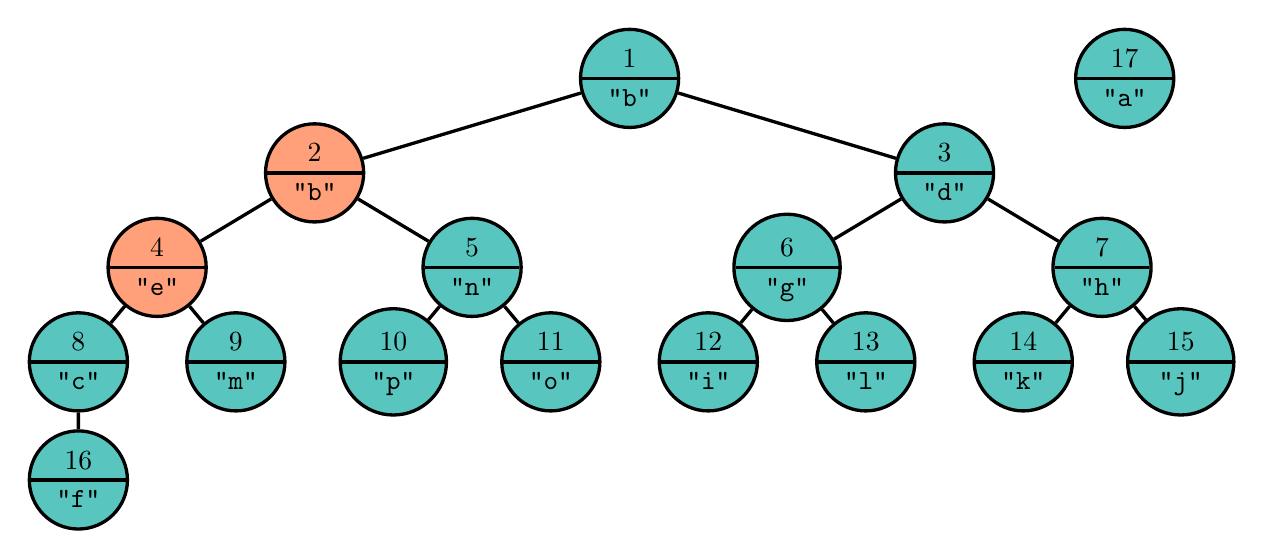
\begin{tikzpicture}[very thick,level 1/.style={sibling distance=80mm}, level 2/.style={sibling distance=40mm}, level 3/.style={sibling distance=20mm}, level distance=12mm, level 4/.style={level distance=15mm}]
\node [splitvertex] (r){1\nodepart{lower}\texttt{"b"}}
  child {
    node [splitvertex, fill=mysalmon] (a) {2\nodepart{lower}\texttt{"b"}}
    child {
      node [splitvertex, fill=mysalmon] {4\nodepart{lower}\texttt{"e"}}
      child {
        node [splitvertex] {8\nodepart{lower}\texttt{"c"}}
        child {node [splitvertex] {16\nodepart{lower}\texttt{"f"}}}
      } 
      child {
        node [splitvertex] {9\nodepart{lower}\texttt{"m"}}
      }
    }
    child {
      node [splitvertex] {5\nodepart{lower}\texttt{"n"}}
      child {node [splitvertex] {10\nodepart{lower}\texttt{"p"}}}
      child {node [splitvertex] {11\nodepart{lower}\texttt{"o"}}}
    }
  }
  child {
    node [splitvertex] {3\nodepart{lower}\texttt{"d"}}
    child {
      node [splitvertex] {6\nodepart{lower}\texttt{"g"}}
      child {node [splitvertex] {12\nodepart{lower}\texttt{"i"}}}
      child {node [splitvertex] {13\nodepart{lower}\texttt{"l"}}}
    }
    child {
      node [splitvertex] {7\nodepart{lower}\texttt{"h"}}
      child {node [splitvertex] {14\nodepart{lower}\texttt{"k"}}}
      child {node [splitvertex] {15\nodepart{lower}\texttt{"j"}}}
    }
  };
  \node [splitvertex] [right=5cm of r]{17\nodepart{lower}\texttt{"a"}};
\end{tikzpicture}
\end{center}

\begin{center}
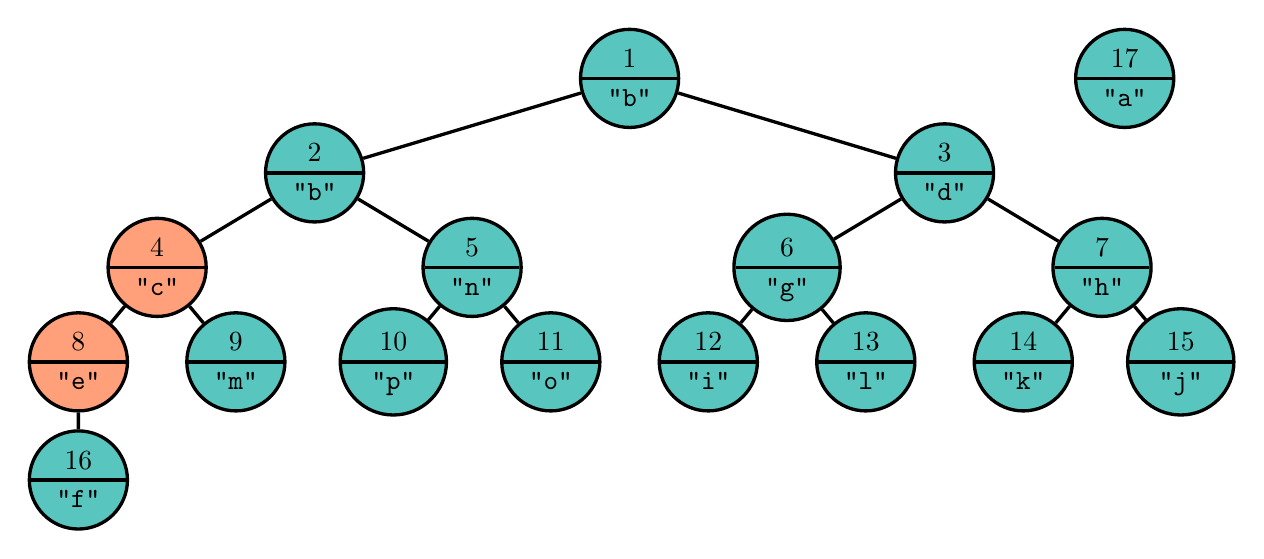
\begin{tikzpicture}[very thick,level 1/.style={sibling distance=80mm}, level 2/.style={sibling distance=40mm}, level 3/.style={sibling distance=20mm}, level distance=12mm, level 4/.style={level distance=15mm}]
\node [splitvertex] (r){1\nodepart{lower}\texttt{"b"}}
  child {
    node [splitvertex] (a) {2\nodepart{lower}\texttt{"b"}}
    child {
      node [splitvertex, fill=mysalmon] {4\nodepart{lower}\texttt{"c"}}
      child {
        node [splitvertex, fill=mysalmon] {8\nodepart{lower}\texttt{"e"}}
        child {node [splitvertex] {16\nodepart{lower}\texttt{"f"}}}
      } 
      child {
        node [splitvertex] {9\nodepart{lower}\texttt{"m"}}
      }
    }
    child {
      node [splitvertex] {5\nodepart{lower}\texttt{"n"}}
      child {node [splitvertex] {10\nodepart{lower}\texttt{"p"}}}
      child {node [splitvertex] {11\nodepart{lower}\texttt{"o"}}}
    }
  }
  child {
    node [splitvertex] {3\nodepart{lower}\texttt{"d"}}
    child {
      node [splitvertex] {6\nodepart{lower}\texttt{"g"}}
      child {node [splitvertex] {12\nodepart{lower}\texttt{"i"}}}
      child {node [splitvertex] {13\nodepart{lower}\texttt{"l"}}}
    }
    child {
      node [splitvertex] {7\nodepart{lower}\texttt{"h"}}
      child {node [splitvertex] {14\nodepart{lower}\texttt{"k"}}}
      child {node [splitvertex] {15\nodepart{lower}\texttt{"j"}}}
    }
  };
  \node [splitvertex] [right=5cm of r]{17\nodepart{lower}\texttt{"a"}};
\end{tikzpicture}
\end{center}

And we are done. Once again, this takes at most $\log(N)$ swaps. This idea can be extended to removing or changing the value of any node we'd like from a tree -- this is particularly useful for Dijkstra later.

Remember to implement your heap in an array or ArrayList!

\begin{itemize}

\item \texttt{boolean add(String s)}

\item \texttt{boolean isEmpty()}

\item \texttt{String poll()}

\item \texttt{String peek()}

\item \texttt{int size()}

\end{itemize}

\section{Set}

A Set is a collection of objects with no duplicate elements. Set is a Java interface. Note that the data structures discussed in this section can be extended to become multisets, but Java implementations of these explicitly disallow multiplicity.

\subsection{TreeSet}

A TreeSet is Java's implementation of a \textit{binary search tree} (BST). A binary search tree is a tree where every node is greater than every node in its left subtree and less than every node in its right subtree. As with a heap, to use a BST, we need to impose some kind of ordering on the elements stored.

\begin{center}
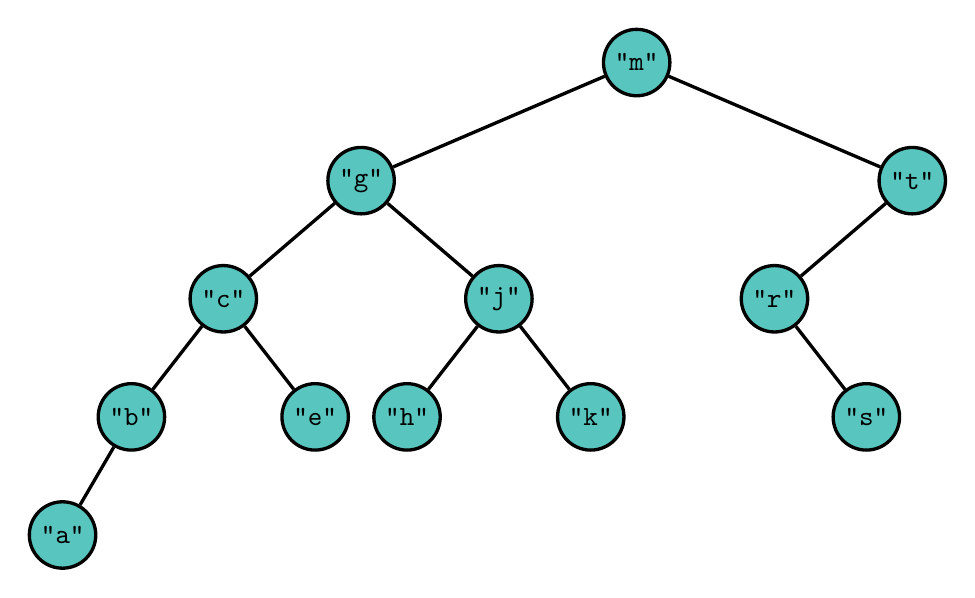
\begin{tikzpicture}[very thick,level/.style={sibling distance=70mm/#1}]
\node [vertex] (r){\texttt{"m"}}
  child {
    node [vertex] {\texttt{"g"}}
    child {
      node [vertex] {\texttt{"c"}}
      child {
        node [vertex] {\texttt{"b"}}
        child {node [vertex] {\texttt{"a"}}}
        child[missing]
      } 
      child {
        node [vertex] {\texttt{"e"}}
      }
    }
    child {
      node [vertex] {\texttt{"j"}}
      child {node [vertex] {\texttt{"h"}}}
      child {node [vertex] {\texttt{"k"}}}
    }
  }
  child {
    node [vertex] {\texttt{"t"}}
    child {
      node [vertex] {\texttt{"r"}}
      child[missing]
      child {node [vertex] {\texttt{"s"}}}
    }
    child[missing]
  };
\end{tikzpicture}
\end{center}

The tree need not be complete. Because it is not complete, there is no way to nicely bound the size of the array we would need if we were to use the same storage method as with the heap. Thus, we are forced to use a TreeNode, with left and right pointers. This is also problematic when determining guarantees on time complexities later, but the ways to solve this problem are pretty complicated so we'll ignore them for now.

Given the name of the tree, searching for an element within the tree is quite natural, and similar to a binary search. Compare the element to be searched for with the current node. If they are equal, we are done; otherwise, search the appropriate left or right subtree. As with most structures and algorithms with a binary search structure, this operation lends itself nicely to recursion. If the tree is reasonably nice, we expect to complete this in $O(\log{n})$ time, but searching can be as bad as linear if the tree looks like a LinkedList.

Adding an element is also natural. As our tree represents a set, it will not contain the same element twice. We trace down until we hit a null pointer, and add the element in the appropriate spot. Let's add a \texttt{"p"} to the BST:

\begin{center}
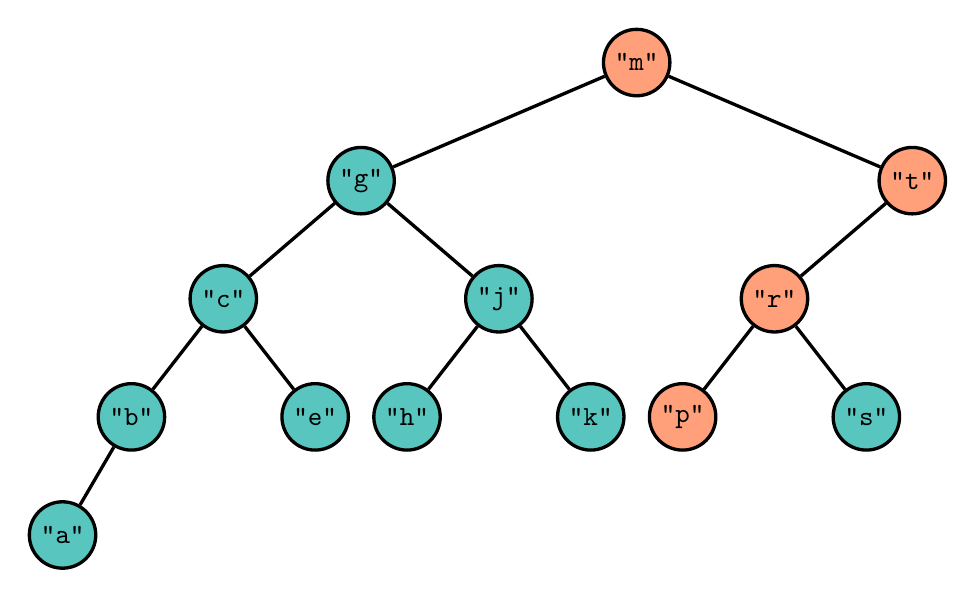
\begin{tikzpicture}[very thick,level/.style={sibling distance=70mm/#1}]
\node [vertex, fill=mysalmon] (r){\texttt{"m"}}
  child {
    node [vertex] {\texttt{"g"}}
    child {
      node [vertex] {\texttt{"c"}}
      child {
        node [vertex] {\texttt{"b"}}
        child {node [vertex] {\texttt{"a"}}}
        child[missing]
      } 
      child {
        node [vertex] {\texttt{"e"}}
      }
    }
    child {
      node [vertex] {\texttt{"j"}}
      child {node [vertex] {\texttt{"h"}}}
      child {node [vertex] {\texttt{"k"}}}
    }
  }
  child {
    node [vertex, fill=mysalmon] {\texttt{"t"}}
    child {
      node [vertex, fill=mysalmon] {\texttt{"r"}}
      child {node [vertex, fill=mysalmon] {\texttt{"p"}}}
      child {node [vertex] {\texttt{"s"}}}
    }
    child[missing]
  };
\end{tikzpicture}
\end{center}

Deleting an element is the annoying part. Unfortunately, there's not much we can do besides casework.

Removing a leaf, like \texttt{"a"}, from the tree is very easy. Removing a node with only once child, like \texttt{"t"}, is also relatively straightforward.

\begin{center}
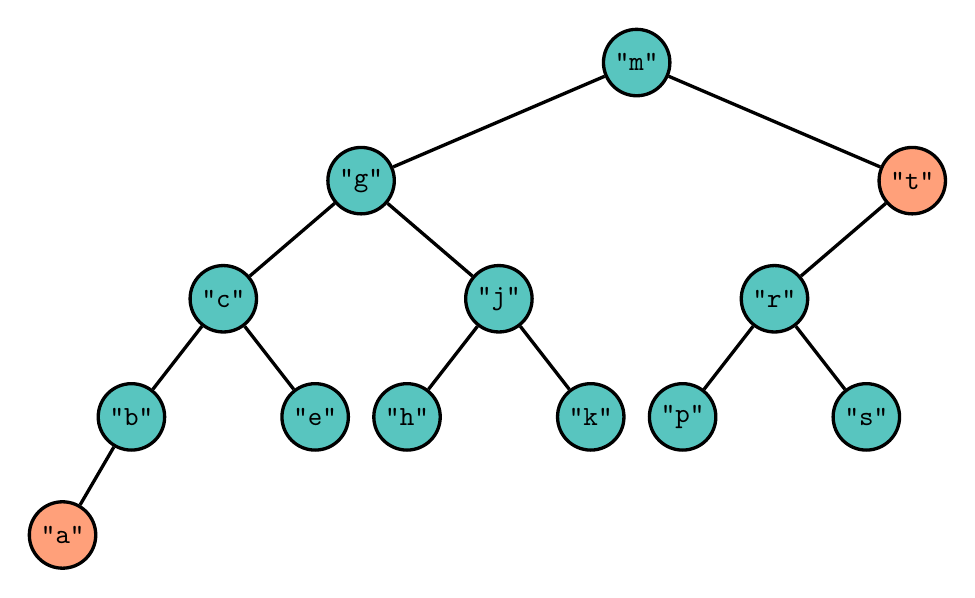
\begin{tikzpicture}[very thick,level/.style={sibling distance=70mm/#1}]
\node [vertex] (r){\texttt{"m"}}
  child {
    node [vertex] {\texttt{"g"}}
    child {
      node [vertex] {\texttt{"c"}}
      child {
        node [vertex] {\texttt{"b"}}
        child {node [vertex,fill=mysalmon] {\texttt{"a"}}}
        child[missing]
      } 
      child {
        node [vertex] {\texttt{"e"}}
      }
    }
    child {
      node [vertex] {\texttt{"j"}}
      child {node [vertex] {\texttt{"h"}}}
      child {node [vertex] {\texttt{"k"}}}
    }
  }
  child {
    node [vertex, fill=mysalmon] {\texttt{"t"}}
    child {
      node [vertex] {\texttt{"r"}}
      child {node [vertex] {\texttt{"p"}}}
      child {node [vertex] {\texttt{"s"}}}
    }
    child[missing]
  };
\end{tikzpicture}
\end{center}

Now, removing an element with two children is tricky. We'll try to remove \texttt{"g"}. Consider the least element in the right subtree of \texttt{"g"}, which in this case is \texttt{"h"}. We find \texttt{"h"} by always choosing the left child on the right subtree until we cannot go any further. This must be the least element.

\begin{center}
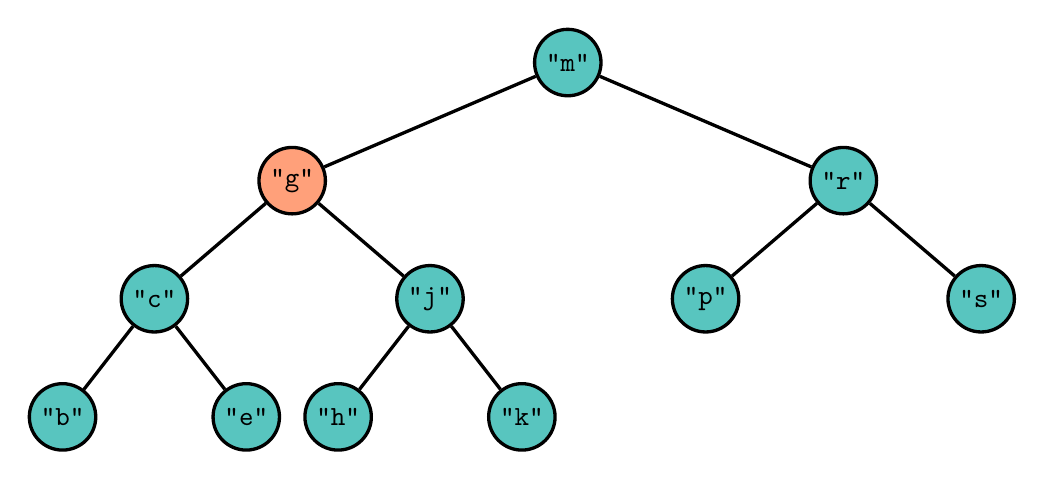
\begin{tikzpicture}[very thick,level/.style={sibling distance=70mm/#1}]
\node [vertex] (r){\texttt{"m"}}
  child {
    node [vertex, fill=mysalmon] {\texttt{"g"}}
    child {
      node [vertex] {\texttt{"c"}}
      child {
        node [vertex] {\texttt{"b"}}
      } 
      child {
        node [vertex] {\texttt{"e"}}
      }
    }
    child {
      node [vertex] {\texttt{"j"}}
      child {node [vertex] {\texttt{"h"}}}
      child {node [vertex] {\texttt{"k"}}}
    }
  }
  child {
      node [vertex] {\texttt{"r"}}
      child {node [vertex] {\texttt{"p"}}}
      child {node [vertex] {\texttt{"s"}}}
  };
\end{tikzpicture}
\end{center}

Note that \texttt{"h"} has either no children or only one child, and that nodes like these are easy to remove. We then change the value of the node containing \texttt{"g"} to \texttt{"h"}, which is legal since \texttt{"h"} is the least element, and remove \texttt{"h"} from the right subtree, and we are done.

\begin{center}
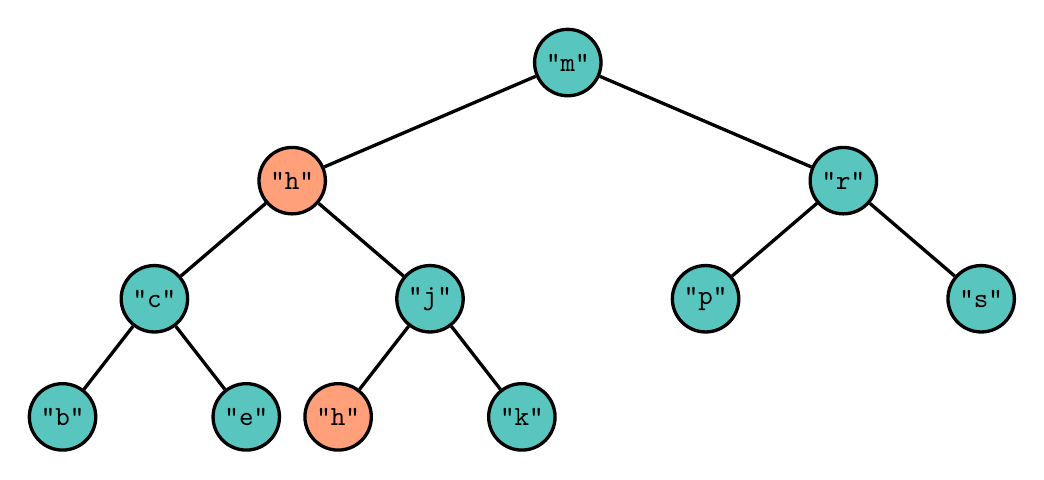
\begin{tikzpicture}[very thick,level/.style={sibling distance=70mm/#1}]
\node [vertex] (r){\texttt{"m"}}
  child {
    node [vertex, fill=mysalmon] {\texttt{"h"}}
    child {
      node [vertex] {\texttt{"c"}}
      child {
        node [vertex] {\texttt{"b"}}
      } 
      child {
        node [vertex] {\texttt{"e"}}
      }
    }
    child {
      node [vertex] {\texttt{"j"}}
      child {node [vertex, fill=mysalmon] {\texttt{"h"}}}
      child {node [vertex] {\texttt{"k"}}}
    }
  }
  child {
      node [vertex] {\texttt{"r"}}
      child {node [vertex] {\texttt{"p"}}}
      child {node [vertex] {\texttt{"s"}}}
  };
\end{tikzpicture}
\end{center}

\begin{center}
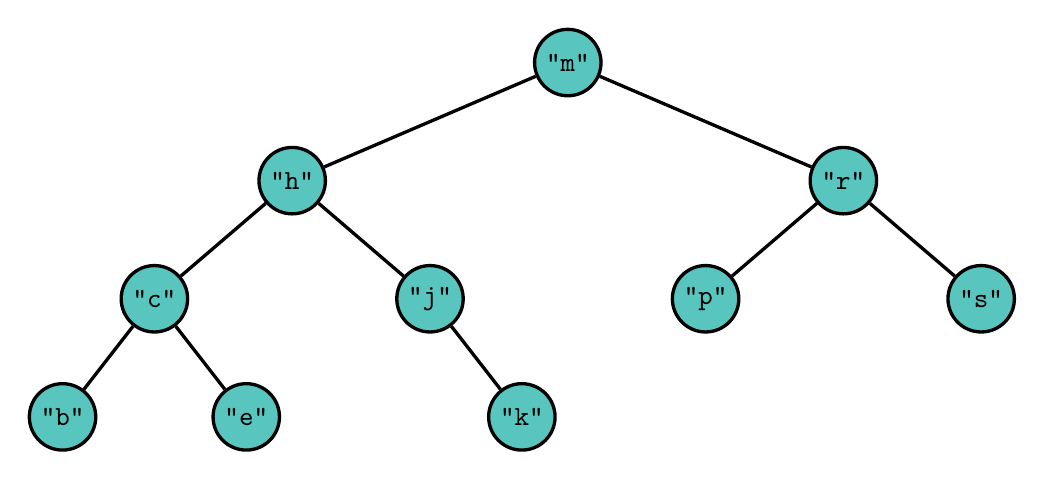
\begin{tikzpicture}[very thick,level/.style={sibling distance=70mm/#1}]
\node [vertex] (r){\texttt{"m"}}
  child {
    node [vertex] {\texttt{"h"}}
    child {
      node [vertex] {\texttt{"c"}}
      child {
        node [vertex] {\texttt{"b"}}
      } 
      child {
        node [vertex] {\texttt{"e"}}
      }
    }
      child {node [vertex] {\texttt{"j"}}
      	child[missing]
        child {
        	node[vertex]{\texttt{"k"}}
        }
      }
  }
  child {
      node [vertex] {\texttt{"r"}}
      child {node [vertex] {\texttt{"p"}}}
      child {node [vertex] {\texttt{"s"}}}
  };
\end{tikzpicture}
\end{center}

A standard BST has $O(\log{n})$ operations if the tree is ``nice'', but each operation can be $O(n)$ in the worst case. We need to find a way to automatically balance the BST such that we avoid linear time complexities.

A red-black tree is a self-balancing BST that guarantees $O(\log{n})$ operations by making sure the height of the tree grows logarithmically. It is implemented in Java's TreeSet, so while the BST I described above does not guarantee nice time bounds, Java's implementation does.

I don't think learning exactly how a red-black tree works is particularly useful for the beginning programmer. How exactly a red-black tree works, together with some more balanced binary search trees which are useful on the competitive scene, are covered in a later chapter.

Here are some notable functions TreeSet implements. You don't need to implement everything -- \texttt{add()}, \texttt{remove()}, and \texttt{contains()} are the most important.

\begin{itemize}

\item
\texttt{boolean add(String s)}

\item
\texttt{String ceiling(String s)} -- the least element in the set greater than or equal to \texttt{s}, or \texttt{null} if there is no such element.

\item
\texttt{boolean contains(Object o)}

\item
\texttt{String first()} -- the least element in the set.

\item
\texttt{String floor(String s)} -- the greatest element in the set less than or equal to \texttt{s}, or \texttt{null} if there is no such element.

\item
\texttt{String higher(String s)} -- the least element in the set strictly greater than \texttt{s}, or \texttt{null} if there is no such element.

\item
\texttt{boolean isEmpty()}

\item
\texttt{String last()} -- the greatest element in the set.

\item
\texttt{String lower(String s)} -- the greatest element in the set strictly less than \texttt{s}, or \texttt{null} if there is no such element.

\item
\texttt{boolean remove(Object o)}

\item
\texttt{int size()}

\end{itemize}

Since the TreeSet is ordered, iterating over a TreeSet will also be in order.

\subsection{HashSet}

A HashSet is a way for us to store objects when we do not require a natural ordering on the set. As with the TreeSet, we want to be able to check whether an element is in our set or not quickly. We do this with the help of a \textit{hash function}. Every Java Object supports the \texttt{hashCode()} function. We usually want to map an object with an integer hash, so that we can store the values in an array. For example, let us define the following hash for Strings:

\begin{mylstlisting}
public int hashCode() {
	int hash = 0;
    for(int k = 0; k < length(); k++) {
		hash *= 31;
        hash += (int) (charAt(k));
    }
    return hash;
}
\end{mylstlisting}

\texttt{a.equals(b)} should imply \texttt{a.hashCode() == b.hashCode()}. This function produces the same result as the actual \texttt{hashCode()} function in the String class. However, this is not quite what we want for our HashSet, because in the end we wish to be able to store the objects in some kind of array. This hash not only returns integers that can be very large, they can also be negative, and thus are not suitable as array indices. The natural way to fix this is to take the hash modulo the size of the array we want.

\begin{mylstlisting}
String[] table = new String[10007];
int index(String s) {
	int i = s.hashCode() % table.length;
    if(i >= 0)
    	return i;
	return i + table.length;
}
\end{mylstlisting}

We chose the number 10007 because it is a prime number, and primes are generally nice when taking a number modulo something else, as integers modulo a prime form a field. Remember that a negative number \texttt{\%} another number is not necessarily positive, so we need to be a little careful.

From here, adding an element to the HashSet and checking if an element is contained both seem straightforward:

\begin{mylstlisting}
boolean add (String s) {
	table[index(s)] = s;
    return true;
}
boolean contains(Object o) {
    int i = index((String) o);
	return table[i] != null && table[i].equals(o);
}
\end{mylstlisting}

\texttt{null} is always annoying to deal with, and will have to be handled separately.

However, one problem quickly arises. Two Strings may map to the same index in the array. We call this a \textit{collision}. The easiest way to handle a collision is by \textit{chaining}. We change the hash table to store a LinkedList instead of a single element in the event of a collision. Java once implemented this method of resolving collisions, but recently changed the LinkedList to a BST in Java 8.

\begin{itemize}

\item
\texttt{boolean add(String s)}

\item
\texttt{boolean contains(Object o)}

\item
\texttt{boolean isEmpty()}

\item
\texttt{boolean remove(Object o)}

\item
\texttt{int size()}

\end{itemize}

\section{Map}

A Map is simply an extension of a Set. It stores a mapping that takes a key to a value. Map is a Java Interface. Generics for Maps therefore have two arguments. Consider the following Map from Strings to Integers.

\begin{mylstlisting}
Map<String, String> email = new TreeMap<String, String>();
m.put("Samuel Hsiang", "samuel.c.hsiang@gmail.com");
\end{mylstlisting}

The keys of a Map form a Set, though the Values need not be unique.

The TreeMap is the Map variant of the TreeSet; similarly, the HashMap is the Map variant of the HashSet.

All useful Set functions have a Map counterpart. The following additional functions are of use.

\begin{itemize}

\item
\texttt{Set<String> keySet()} -- returns the set of keys.

\item
\texttt{Integer put(String k, String v)} -- assigns the value \texttt{k} to the key \texttt{v}, and returns the old value assigned to \texttt{k}.

\end{itemize}

\section{BigInteger}

BigInteger is in \texttt{java.math} for times when int and long just aren't large enough. The way BigInteger works is it stores a number as an array of ints. Each value in the array represents a digit in some very large base. Addition and subtraction can be done in the standard way. Generally multiplying two BigIntegers is not necessary on contests, but it can be sped up using Karatsuba or the FFT.

\section{C++ Analogs}

\begin{itemize}

\item \texttt{ArrayList} -- \texttt{vector}
\item \texttt{LinkedList} -- \texttt{list} or \texttt{deque}
\item \texttt{Stack} -- \texttt{stack}
\item \texttt{Queue} -- \texttt{queue}
\item \texttt{PriorityQueue} -- \texttt{priority\_queue}, but note that \texttt{priority\_queue} pops \textit{max} element first
\item \texttt{TreeSet} -- \texttt{set}
\item \texttt{HashSet} -- \texttt{unordered\_set}, C++11
\item \texttt{TreeMap} -- \texttt{map}
\item \texttt{HashMap} -- \texttt{unordered\_map}, C++11
\item \texttt{BigInteger} -- no equivalent

\end{itemize}

\chapter{Big Ideas}

In this chapter we'll discuss some general ideas for solving problems. Starting in this chapter I'm going to shift from language-specific terms, like PriorityQueue and TreeMap, to more general terms, like binary heap and binary search tree. Algorithms I present will no longer be in the form of concrete Java code but rather in a more abstract pseudocode.

\section{Search Techniques}

There are many different general strategies for finding the answer to a problem.

\subsection{Complete Search}

Sometimes the best way is simply to try everything. This could be the intended solution (check the complexity of a complete search and compare it against the time limits), or we may be just coding a brute force to squeeze out a few extra points from an intractable problem at the end of a contest. Either way, the order in which we search can make or break the code.

Suppose we wanted to solve the game of chess. The placement of the pieces on the board and a toggle for whether black or white is to move represents a game state. The set of legal moves maps this game state to one set of states and another set of states to this game state.

We can therefore think of the different states as vertices in a very large directed graph. Methods we use for solving chess, or any other problem, are identical to ways of traversing graphs, especially trees.

\subsubsection{Depth-First Search}

\textit{Depth-first search} is the most simple of the searches. A depth-first search called on a vertex $v$ in the search tree recursively calls itself on each of the children of $v$. To go back to the chess example, a DFS would begin with one possible first move, like a3, and test \textit{every possible move sequence} beginning with a3 before moving on to a second possible first move, like a4.

A quick note on recursive processes: The \textit{run-time stack} keeps track of our position and data that go out of scope when we jump into a new function. This stack allows us to call functions within functions safely. Recursion is dangerous in contest programming because the run-time stack is slow and can easily balloon in size, crashing the program. For this reason do not hesitate to use your own stack in an iterative process in practice, though I often describe processes as recursive as they are easier to understand, code, and debug in this form.

Now it is painfully obvious that strictly using a DFS is not preferable in computer chess. The computer would certainly never finish testing every move sequence beginning with a3 and therefore would not consider more standard, and likely better, moves like e4.

\subsubsection{Breadth-First Search}

\textit{Breadth-first search} traverses the search tree level by level. We keep track of a queue that stores each level's state. At each step we pop off the first element in the queue and add the states that it can reach to the end of the queue. In this way, we explore those states only after we explore all the states associated with a lower level. In the chess example, we would store all 20 possible first moves in the queue, and for each first move, we add all possible second moves to the end of the queue.

This means that we search all possible states of a certain depth at roughly the same time, but we need to store the data associated with each of these states, and this can be quite costly in terms of memory.

BFS is the better choice over DFS when we are asked for the ``smallest'' answer, which is often associated with the lowest level.

\subsubsection{Depth-First Search with Iterative Deepening}

\textit{Depth-first search with iterative deepening} is a DFS that only searches up to a certain level in the search tree before stopping and heading back to lower levels. If it turns out the search did not find anything in the first $N$ levels, we broaden the search to the first $N+1$ levels with another DFS, hence iterative deepening. This method of searching is slower than a BFS, but maintains the nice BFS property of finding the ``smallest'' answer first while shedding the memory harness that holds the BFS back.

DFSID is the closest to what we do when analyzing an actual chess game. We make a move in our minds and test its performance against whatever the opponent might make as his move, tracing the game around 3-4 moves deep before testing another possible move.

\subsection{Greedy Algorithm}

The main problem with any of the searches described above is they are exponential in nature. A \textit{greedy algorithm} is one that takes the ``best'' possible option at each step, essentially disregarding any other possible option. To find the best solution for $n=4$, we consider only the best solution for $n=3$ and no other possible solution. The approach of maximizing at each step clearly does not always work, as the locally optimal choice is not necessarily globally optimal. Always moving in the direction of a target, for example, fails if there is a wall in the way. However, if the greedy algorithm can solve a problem, the code runs very quickly.

One problem that cannot be solve using the greedy approach is the integer knapsack problem. It's important to be able to catch an incorrect greedy algorithm, and one classic
example involves finding the most efficient way to make change. Given a sequence of coin denominations ($d_i$, where $1 \le i \le n$), with $d_1 = 1$, find the smallest number of coins necessary that sum to some value $V$. The greedy approach takes the most valuable coin that doesn't overshoot $V$ and adds it to our set until we achieve $V$. One counterexample is $v_1=1$, $v_2=3$, $v_3=4$ and $V = 6$. The greedy algorithm chooses $4+1+1$, which is worse than $3+3$. Note however that greedy algorithm still always works for some sets of coin values, like United States currency. Don't let the fact that the greedy algorithm works for the most obvious example fool you.

The greedy algorithm combined with ideas from dynamic programming constitute \textit{best-first search}, a category of searches that includes the Dijkstra algorithm for shortest paths.

\begin{enumerate}

\item
(USACO Training)
There is a long list of stalls, some of which need to be covered with boards. You can use up to $N$ ($1 \le N \le 50$) boards, each of which may cover any number of consecutive stalls. Cover all the necessary stalls, while covering as few total stalls as possible.

\item
(IOI 1996)
You are given a three-valued (1, 2, or 3) sequence of length up to 1000. Find a minimum set of exchanges to put the sequence in sorted order.

\item
(Samir Khuller)
We are given $N$ jobs, each of which requires one unit of time to complete. The $i$th job opens at some time $t_i$ and must be completed by some deadline $d_i$, where $t_i,d_i\in \mathbb{Z}$. Given that only one job can be completed at a time, determine if all $N$ can be completed by their deadlines.

\end{enumerate}

\subsection{Binary Searching on the Answer}

Suppose that the problem we need to solve is finding the minimum number $M$ such that some property holds. That is, the property holds for any $x \ge M$ but does not hold for $x < M$. Perhaps the best approach we have so far for finding this $M$ is simply trying all the numbers from 1 to $M$. However, this linear search is clearly inefficient.

The nature of this problem should remind you of some other search technique. Oftentimes, with problems of this property, it is easy to check whether some condition holds for some given $x$. In this case, it is much easier to binary search on $M$ rather than find it some other way.

\begin{enumerate}

\item
(USACO March 2014, sabotage)
Farmer John's arch-nemesis, Farmer Paul, has decided to sabotage Farmer
John's milking equipment!

The milking equipment consists of a row of $N$ ($3 \le N \le 100,000$)
milking machines, where the $i$th machine produces $M_i$ units of milk ($1 \le M_i \le 10,000$).  Farmer Paul plans to disconnect a contiguous block
of these machines -- from the $i$th machine up to the $j$th machine ($2 \le i \le j \le N-1$); note that Farmer Paul does not want to disconnect
either the first or the last machine, since this will make his plot
too easy to discover.  Farmer Paul's goal is to minimize the average
milk production of the remaining machines.  Farmer Paul plans to
remove at least 1 cow, even if it would be better for him to avoid
sabotage entirely.

Fortunately, Farmer John has learned of Farmer Paul's evil plot, and
he is wondering how bad his milk production will suffer if the plot
succeeds.  Please help Farmer John figure out the minimum average milk
production of the remaining machines if Farmer Paul does succeed.

\item
(Matthew Savage)
Ashley's journey through Unova is just beginning, and she has just picked her first Pok\'{e}mon! Unfortunately, not knowing much about them, she picked a Snivy, and a particularly stubborn and unfriendly one at that.

Being Ashley, she decides to try to win over the Snivy in the only way she knows how -- baked goods.

Ashley knows $r$ $(0 \le r \le 1000$) recipes for Pok\'{e}puffs. Each recipe $r_i$ has a deliciousness rating $d_i$ ($0 \le d_i \le 1000$) and requires some combination of the $I$ ($0 \le I \le 1000$) available ingredients. (More specifically, the recipe $r_i$ uses the quantity $I_{ij}$ ($0 \le I_{ij} \le 1000$) of ingredient $I_j$.)

Ashley has some amount of each ingredient $I_j$ on hand $A_j$ ($0 \le A_j \le 10^9$) and can buy more from the nearby store for a price of $c_j$ ($1 \le c_j \le 10^9$) dollars per unit using the $M$ ($0 \le M \le 10^{12}$) dollars she currently has.

Of course, Ashley also has limited supplies and therefore can only produce Pok\'{e}puffs from a single recipe. However, she can make as many as she wants, in integer increments.

We define ``total deliciousness'' ($D$) to be the sum of the deliciousnesses of the individual Poképuffs that Ashley has baked.

Ashley wants to have the best chance possible with Snivy, and therefore would like to know - what is the maximum possible deliciousness ($\max(D)$) that she can produce?

Note: there is a ``just do it'' solution that is faster than the binary search by a log factor. It is also \textit{much} more annoying to code; so annoying that I was unable to debug my ``just do it'' solution in the actual contest environment. I included this problem as an exercise to demonstrate how easy binary searching on the answer can be.

\item
(CF 287B)
Vova, the Ultimate Thule new shaman, wants to build a pipeline. As there are exactly $n$ ($1 \le n \le 10^{18}$) houses in Ultimate Thule, Vova wants the city to have exactly $n$ pipes, each such pipe should be connected to the water supply. A pipe can be connected to the water supply if there's water flowing out of it. Initially Vova has only one pipe with flowing water. Besides, Vova has several splitters.

A splitter is a construction that consists of one input (it can be connected to a water pipe) and $x$ output pipes. When a splitter is connected to a water pipe, water flows from each output pipe. You can assume that the output pipes are ordinary pipes. For example, you can connect water supply to such pipe if there's water flowing out from it. At most one splitter can be connected to any water pipe.

Vova has one splitter of each kind: with $2, 3, 4, \ldots, k$ ($2 \le k \le 10^9$) outputs. Help Vova use the minimum number of splitters to build the required pipeline or otherwise state that it's impossible.

Vova needs the pipeline to have exactly n pipes with flowing out water. Note that some of those pipes can be the output pipes of the splitters.

\item
(IOI 2009)
Mecho the bear has found a little treasure - the bees' secret honeypot, which is full of honey! He was happily eating his newfound treasure until suddenly one bee saw him and sounded the bee alarm. He knows that at this very moment hordes of bees will emerge from their hives and start spreading around trying to catch him. He knows he has to leave the honeypot and go home quickly, but the honey is so sweet that Mecho doesn't want to leave too soon. Help Mecho determine the latest possible moment when he can leave.

Mecho's forest is represented by a square grid of $N$ by $N$ ($1 \le N \le 800$) unit cells, whose sides are parallel to the north-south and east-west directions. Each cell is occupied by a tree, by a patch of grass, by a hive or by Mecho's home. Two cells are considered adjacent if one of them is immediately to the north, south, east or west of the other (but not on a diagonal). Mecho is a clumsy bear, so every time he makes a step, it has to be to an adjacent cell. Mecho can only walk on grass and cannot go through trees or hives, and he can make at most $S$ ($1 \le S \le 1000$) steps per minute. At the moment when the bee alarm is sounded, Mecho is in the grassy cell containing the honeypot, and the bees are in every cell containing a hive (there may be more than one hive in the forest). During each minute from this time onwards, the following events happen in the following order:
\begin{itemize}
\item
If Mecho is still eating honey, he decides whether to keep eating or to leave. If he continues eating, he does not move for the whole minute. Otherwise, he leaves immediately and takes up to $S$ steps through the forest as described above. Mecho cannot take any of the honey with him, so once he has moved he cannot eat honey again.
\item
After Mecho is done eating or moving for the whole minute, the bees spread one unit further across the grid, moving only into the grassy cells. Specifically, the swarm of bees spreads into every grassy cell that is adjacent to any cell already containing bees. Furthermore, once a cell contains bees it will always contain bees (that is, the swarm does not move, but it grows).
\end{itemize}
In other words, the bees spread as follows: When the bee alarm is sounded, the bees only occupy the cells where the hives are located. At the end of the first minute, they occupy all grassy cells adjacent to hives (and still the hives themselves). At the end of the second minute, they additionally occupy all grassy cells adjacent to grassy cells adjacent to hives, and so on. Given enough time, the bees will end up simultaneously occupying all grassy cells in the forest that are within their reach.

Neither Mecho nor the bees can go outside the forest. Also, note that according to the rules above, Mecho will always eat honey for an integer number of minutes.

The bees catch Mecho if at any point in time Mecho finds himself in a cell occupied by bees.

Write a program that, given a map of the forest, determines the largest number of minutes that Mecho can continue eating honey at his initial location, while still being able to get to his home before any of the bees catch him.

\end{enumerate}

\section{Dynamic Programming}

The idea behind dynamic programming is to avoid doing the same thing twice. Two nodes in the search tree described in the complete search techniques might very well represent the same state. For example, two different sets of initial moves could result in the same chessboard configuration, and if we already calculated who has the winning or losing position in that configuration, we ought to remember that fact somehow so we don't need to calculate it again. Of course, however, actually keeping track of every possible game state is intractable by memory constraints.

Here's a much more reasonable problem. Given a sequence of $N \le 10,000$ integers, what is the maximum decreasing subsequence? A subsequence does not have to consist of consecutive terms in the original sequence.

\begin{center}
{
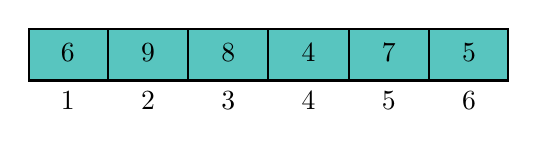
\begin{tikzpicture}[
  thick,
  myrect/.style={
    draw,
    fill=myseagreen,
    rectangle split,
    rectangle split horizontal,
    rectangle split parts=#1,
    rectangle split part align=left,
    text width=5ex,
    text centered
    },
  mycallout/.style={
    shape=rectangle callout,
    rounded corners,
    fill=mysalmon,
    callout absolute pointer={#1},
    callout pointer width=1cm
  }  
]

\node[myrect=6]
  (array)
  {
  					\strut 6
  \nodepart{two}	\strut 9
  \nodepart{three}	\strut 8
  \nodepart{four}	\strut 4
  \nodepart{five}	\strut 7
  \nodepart{six}	\strut 5
  };
\foreach \Valor [count=\Valori from 1] in {one ,two ,three , four , five , six }
  \node[below] at (array.\Valor south) {\Valori};

\end{tikzpicture}
}
\end{center}

The natural complete search approach would be to use recursion, or DFS. When we process an element in the list, we recursively process all elements that come after it and choose the one that gives the maximum subsequence.

\begin{algorithmic}
\Function{Process}{$i$}
\State $max \gets 0$
\For{$j\equiv i+1,N$}
	\If{$value(i) > value(j)$}
		\State $x \gets \Call{Process}{$j$}$
		\If{$x > max$}
			\State $max \gets x$
		\EndIf
	\EndIf
\EndFor
\State \Return $max + 1$
\EndFunction
\end{algorithmic}

However, this algorithm is exponential. In the worst case, it is $O(2^N)$. We notice a lot of repetition: processing the 9 in the list above, for example, requires finding the longest subsequences beginning with 8, 4, 7, and 5, while processing 8 requires finding subsequences for 4, 7, and 5. It seems silly to do the same task twice, so we'll keep track of the length of the longest subsequence in a separate array.

\begin{algorithmic}
\Function{Process}{$i$}
\If{$i$ has already been processed}
	\State \Return $dp(i)$
\EndIf
\State $max \gets 0$
\For{$j\equiv i+1,N$}
	\If{$value(i) > value(j)$}
		\State $x \gets \Call{Process}{j}$
		\If{$x > max$}
			\State $max \gets x$
		\EndIf
	\EndIf
\EndFor
\State $dp(i) \gets max + 1$
\State \Return $max + 1$
\EndFunction
\end{algorithmic}

This reduces the complexity of the algorithm to $O(n^2)$. Note that to process an index, we must process first all later indices. This imposes a natural ordering in which to process the indices: in reverse. This idea lends itself to a nice iterative solution.

\begin{algorithmic}
\For{$i \equiv N,1$}
	\Comment $i$ goes in reverse
	\State $max \gets 0$
	\For{$j\equiv i+1,N$}
		\If{$value(i) > value(j)$}
			\If{$dp(j) > max$}
				\State $max \gets dp(j)$
			\EndIf
		\EndIf
	\EndFor
	\State $dp(i) \gets max + 1$
\EndFor
\end{algorithmic}

The answer to the original problem is then the maximum value of $dp(i)$ for all $i$. For this specific problem, it's relatively easy to speed up the algorithm to $O(\log{n})$ by replacing the linear search with something else.

The integer knapsack problem is another example where dynamic programming may be useful. \textit{Knapsack problems} are a family of problems with the following form:

We are given a list of $K$ objects each assigned an availability, a size, and a value. We have a total amount of ``space'' available in our knapsack and need to find the set of objects from our list that maximizes the total the value of objects in the set such that the total size does not exceed the space and the number of times we take one particular object does not exceed its availability.

Dynamic programming yields a straightforward $O(NK)$ solution. See if you can find it. Note, however, if $N$ is very large, this solution is no longer practical. In general, the knapsack problem is NP-complete, so don't think dynamic programming works on everything!

\subsection{Dynamic Programming over Subsets}

Consider the following problem:

(USACO December 2014, guard)
Farmer John and his herd are playing frisbee.  Bessie throws the
frisbee down the field, but it's going straight to Mark the field hand
on the other team!  Mark has height $H$ ($1 \le H \le 1,000,000,000$), but
there are $N$ cows on Bessie's team gathered around Mark ($2 \le N \le 20$).
They can only catch the frisbee if they can stack up to be at least as
high as Mark.  Each of the $N$ cows has a height, weight, and strength.
A cow's strength indicates the maximum amount of total weight of the
cows that can be stacked above her.  

Given these constraints, Bessie wants to know if it is possible for
her team to build a tall enough stack to catch the frisbee, and if so,
what is the maximum safety factor of such a stack.  The safety factor
of a stack is the amount of weight that can be added to the top of the
stack without exceeding any cow's strength.

We can try the $O(N!)$ brute force, trying every permutation of cows possible. However, this is far too slow. $N \le 20$ hints at an exponential solution, so we think of trying every possible subset of the cows. Given a subset $S$ of cows, the height reached is the same, so perhaps we sort the subset by strength, and put the strongest cow on the bottom. We see that this greedy approach fails: suppose that the first cow has weight 1 and strength 3 and the second cow has weight 4 and strength 2. Greedy would tell us to put the first cow on the bottom, but this fails, while putting the second cow on the bottom succeeds.

When greedy fails, the next strategy we look at is dynamic programming. To decide whether $S$ is stable, we have to find whether there exists a cow $j$ in $S$ that can support the weight of all the other cows in $S$. But how do we know whether the set $S \setminus \{j\}$ is stable? This is where dynamic programming comes in.

This leads to a $O(N 2^N)$ solution. This seems like a pain to code iteratively, but there is a nice fact about subsets: there is a cute bijection from the subsets of $\{0,1,2, \ldots, N-1\}$ to the integers from 0 to $2^N - 1$. That is, the subset $\{0,2,5,7\}$ maps to $2^0 + 2^2 + 2^5 + 2^7 = 165$ in the bijection. We call this technique \textit{masking}. We require all the subsets of $S$ to be processed before $S$ is processed, but that property is also handled by our bijection, since subtracting a power of 2 from a number decreases it. With a little knowledge of bit operators, this can be handled easily.

\begin{algorithmic}
\For{$i\gets 0, 2^N-1$}
	\Comment $i$ represents the subset $S$
	\State $dp(i) \gets -1$
	\ForAll{$j \in S$}
		\Comment \texttt{i \& (1 << j) != 0}
		\State $alt \gets \min(dp(i-2^j), strength(j) - \sum_{k \in S \setminus \{j\}} weight(k))$
		\If{$dp(i) < alt$}
			\State $dp(i) \gets alt$
		\EndIf
	\EndFor
\EndFor
\end{algorithmic}

\texttt{\&} is the bitwise and function, while \texttt{<<} is the left shift operator.

Brian Dean compiled some standard dynamic programming problems with animations and analyses. Practice dynamic programming here: \url{http://people.cs.clemson.edu/~bcdean/dp_practice/}

\chapter{Graph Algorithms}

In this chapter we explore some famous graph theory results.

\section{Connected Components}

A \textit{connected component} of an undirected graph is a subgraph such that, for any two vertices in the component, there exists a path from one to the other. The diagram illustrates three connected components of a graph, where each vertex is colored togethwer with its associated component.

\begin{center}
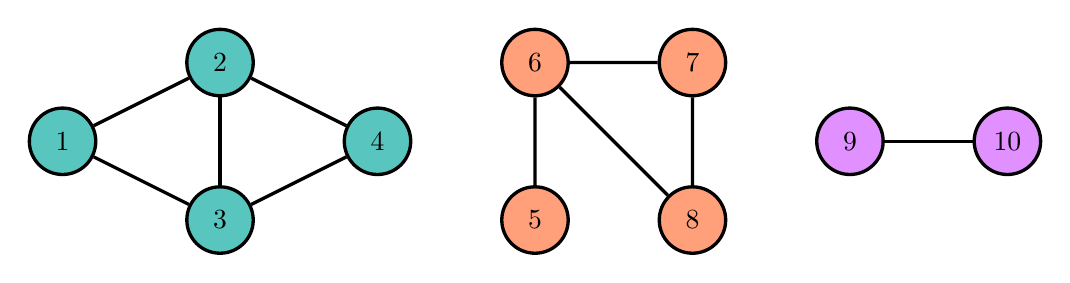
\begin{tikzpicture}[very thick,level/.style={sibling distance=70mm/#1}]
\draw (0, 0) node [vertex] (n1) {1};
\draw (2, 1) node [vertex] (n2) {2};
\draw (2, -1) node  [vertex] (n3) {3};
\draw (4, 0) node [vertex] (n4) {4};
\draw (n1) -- (n2);
\draw (n2) -- (n3);
\draw (n3) -- (n4);
\draw (n2) -- (n4);
\draw (n1) -- (n3);
\draw (6, -1) node [vertex, fill=mysalmon] (n5) {5};
\draw (6, 1) node [vertex, fill=mysalmon] (n6) {6};
\draw (8, 1) node [vertex, fill=mysalmon] (n7) {7};
\draw (8, -1) node [vertex, fill=mysalmon] (n8) {8};
\draw (n5) -- (n6) -- (n7) -- (n8) -- (n6);
\draw (10, 0) node[vertex, fill=mypurple] (n9) {9};
\draw (12, 0) node[vertex, fill=mypurple] (n10) {10};
\draw (n9) -- (n10);
\end{tikzpicture}
\end{center}

A \textit{strongly connected component} of a directed graph is a subgraph such that every vertex in the component can be reached from any other vertex in the component.

\begin{center}
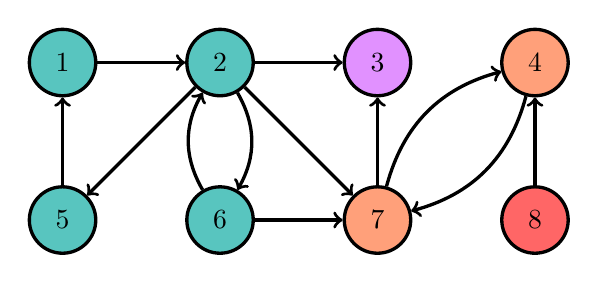
\begin{tikzpicture}[very thick,level/.style={sibling distance=70mm/#1}]
\draw (0, 0) node [vertex] (n1) {5};
\draw (2, 0) node [vertex] (n2) {6};
\draw (4, 0) node [vertex, fill=mysalmon] (n3) {7};
\draw (6, 0) node [vertex, fill=myred] (n4) {8};
\draw (0, 2) node [vertex] (m1) {1};
\draw (2, 2) node [vertex] (m2) {2};
\draw (4, 2) node [vertex, fill=mypurple] (m3) {3};
\draw (6, 2) node [vertex, fill=mysalmon] (m4) {4};
\draw[->] (m1) -- (m2);
\draw[->] (m2) -- (n1);
\draw[->] (n1) -- (m1);
\draw[->] (n2) edge [bend left] (m2);
\draw[->] (m2) edge [bend left] (n2);
\draw[->] (n2) -- (n3);
\draw[->] (m2) -- (m3);
\draw[->] (m2) -- (n3);
\draw[->] (n3) -- (m3);
\draw[->] (n3) edge [bend left] (m4);
\draw[->] (m4) edge [bend left] (n3);
\draw[->] (n4) -- (m4);
\end{tikzpicture}
\end{center}

Finding the connected components of an undirected graph is a straightforward problem, while finding the strongly connected components of a directed graph is more complicated.

\subsection{Flood Fill}

Really any kind of search method solves the undirected graph connected components problem. We could use recursion with a depth-first search. To avoid using the run-time stack, we could use a queue to perform a breadth-first search. Both of these run in $O(E+V)$ time. I would recommend in general to use the BFS.

\subsection{Union-Find}

The union-find data structure is another way for us to solve the connected components problem. Union-find is unique from the other search techniques in that it can process input as it is presented, edge by edge. This also means it is possible to add more edges at the end, therefore changing the graph, while still running quickly. An algorithm that works like this is an \textit{online algorithm}, while an algorithm that requires all the input data presented at the beginning is an \textit{offline algorithm}.

A natural idea for solving the connected components problem is for each vertex to maintain a pointer to another vertex it's connected to, forming a \textit{forest}, or collection of trees. To check whether two elements are in the same component, simply trace the tree up to the root by jumping up each pointer.

\begin{center}
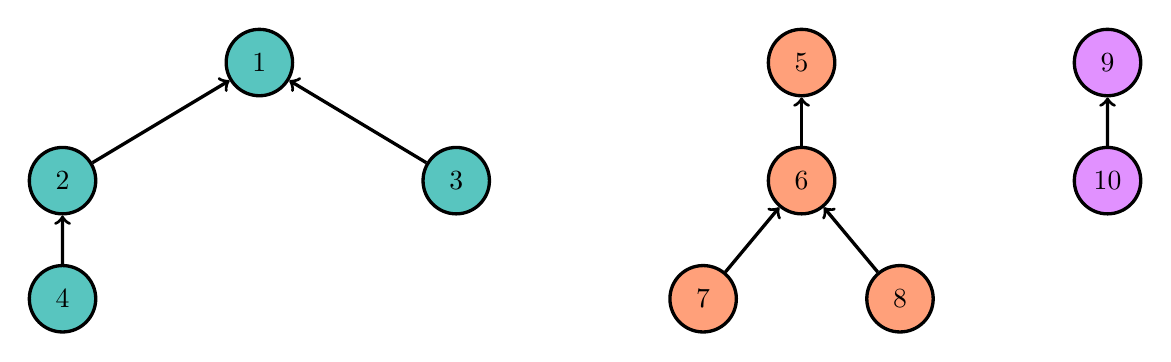
\begin{tikzpicture}[very thick,edge from parent/.style={draw,<-},level/.style={sibling distance=50mm/#1}]
\node [vertex, fill = mysalmon] (r2) {5}
  child {
      node [vertex, fill = mysalmon] {6}
      child { node [vertex, fill=mysalmon] {7} }
      child { node [vertex, fill=mysalmon] {8} }
  };

\node [vertex] [left=6cm of r2] (r1) {1}
  child {
    node [vertex] {2}
    child {
      node [vertex] {4}
    }
  }
  child {node [vertex] {3} };
  
\node [vertex, fill=mypurple] [right=3cm of r2] (r3) {9}
  child { node [vertex, fill=mypurple] {10} };
\end{tikzpicture}
\end{center}

The idea of a pointer can easily be stored within an array.

\begin{center}
{
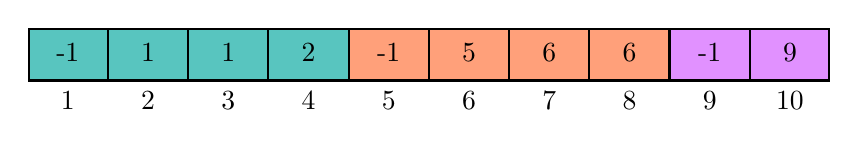
\begin{tikzpicture}[
  thick,
  myrect/.style={
    draw,
    rectangle split,
    rectangle split horizontal,
    rectangle split parts=#1,
    rectangle split part align=left,
    text width=5ex,
    text centered
    },
  mycallout/.style={
    shape=rectangle callout,
    rounded corners,
    fill=mysalmon,
    callout absolute pointer={#1},
    callout pointer width=1cm
  }  
]

\node[myrect=10, rectangle split part fill={myseagreen, myseagreen, myseagreen, myseagreen, mysalmon, mysalmon, mysalmon, mysalmon, mypurple, mypurple}]
  (array1)
  {
  					\strut -1
  \nodepart{two}	\strut 1
  \nodepart{three}	\strut 1
  \nodepart{four}	\strut 2
  \nodepart{five}	\strut -1
  \nodepart{six}	\strut 5
  \nodepart{seven}	\strut 6
  \nodepart{eight}	\strut 6
  \nodepart{nine}	\strut -1
  \nodepart{ten}	\strut 9
  };
\foreach \Valor [count=\Valori from 1] in {one ,two ,three ,four ,five ,six ,seven ,eight ,nine ,ten }
  \node[below] at (array1.\Valor south) {\Valori};

\end{tikzpicture}
}
\end{center}

We want to support two operations: $find(v)$, which returns the root of the tree containing $v$, and $union(u,v)$, which merges the components containing $u$ and $v$. This second operation is easy given the first; simply set the pointer of $find(u)$ to be $find(v)$.

$union(4, 6)$, unoptimized:

\begin{center}
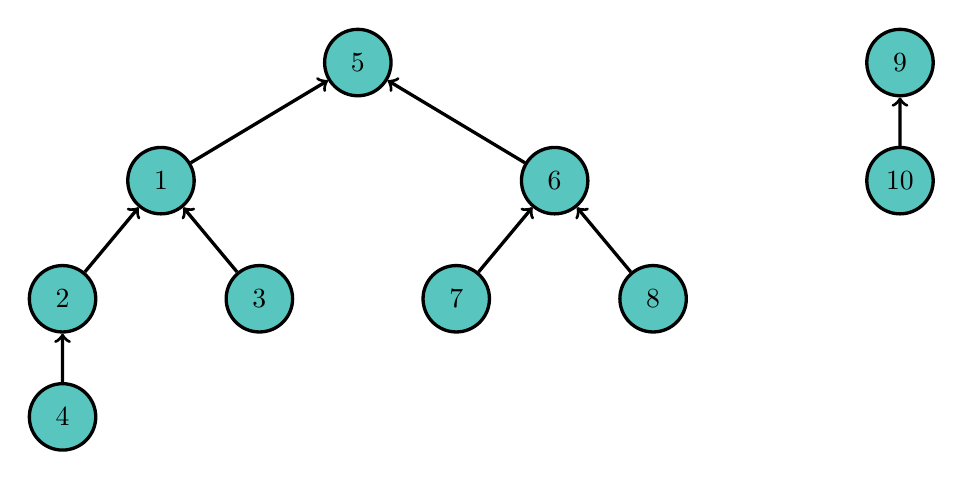
\begin{tikzpicture}[very thick,edge from parent/.style={draw,<-},level/.style={sibling distance=50mm/#1}]
\node [vertex] (r2) {5}
	child {
    node [vertex] (r1) {1}
	  child {
 	   node [vertex] {2}
  	  child {
   	   node [vertex] {4}
  	  }
	  }
 	 child {node [vertex] {3} }
  }
  child {
  node [vertex] {6}
		child { node [vertex] {7} }
   		child { node [vertex] {8} }
    };
\node [vertex] [right=6cm of r2] (r3) {9}
  child { node [vertex] {10} };
\end{tikzpicture}
\end{center}

A problem quickly arises -- the $find$ operation threatens to become linear. There are two simple things we can do to optimize this.

The first is to always add the shorter tree to the taller tree, as we want to minimize the maximum height. An easy heuristic for the height of the tree is simply the number of elements in that tree. We can keep track of the size of the tree with a second array. This heuristic is obviously not perfect, as a larger tree can be shorter than a smaller tree, but it turns out with our second optimization that this problem doesn't matter.

The second fix is to simply assign the pointer associated with $v$ to be $find(v)$ at the end of the $find$ operation. We can design $find(v)$ to recursively call $find$ on the pointer associated with $v$, so this fix sets pointers associated with nodes along the entire chain from $v$ to $find(v)$ to be $find(v)$. These two optimizations combined make the $union$ and $find$ operations $O(\alpha (V))$, where $\alpha(n)$ is the inverse Ackermann function, and for all practical values of $n$, $\alpha(n) < 5$.

$find(4)$, optimized:

\begin{center}
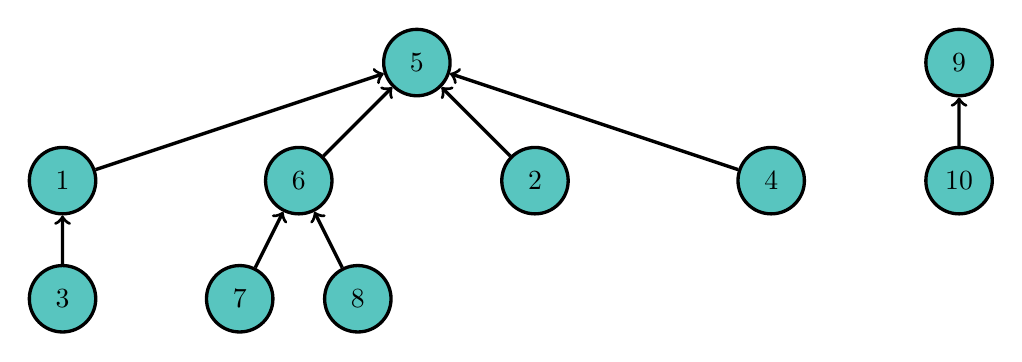
\begin{tikzpicture}[very thick,edge from parent/.style={draw,<-},level/.style={sibling distance=30mm/#1}]
\node [vertex] (r2) {5}
	child {
    node [vertex] (r1) {1}
 	 child {node [vertex] {3} }
  }
  child {
  node [vertex] {6}
		child { node [vertex] {7} }
   		child { node [vertex] {8} }
    }
  child {node[vertex] {2}}
  child {node[vertex] {4}};
\node [vertex] [right=6cm of r2] (r3) {9}
  child { node [vertex] {10} };
\end{tikzpicture}
\end{center}

\begin{algorithm}[H]
\caption{Union-Find}
%\label{}
\begin{algorithmic}
\Function{Find}{$v$}
	\If {$v$ is the root}
		\State \Return $v$
    \EndIf
    \State $parent(v) \gets \Call{Find}{parent(v)}$
    \State \Return $parent(v)$
\EndFunction
\Function{Union}{$u$, $v$}
	\State $uRoot \gets \Call{Find}{u}$
	\State $vRoot \gets \Call{Find}{v}$
    \If {$uRoot = vRoot$}
		\State \Return
	\EndIf
    \If {$size(uRoot)<size(vRoot)$}
    	\State $parent(uRoot) \gets vRoot$
        \State $size(vRoot) \gets size(uRoot) + size(vRoot)$
    \Else
    	\State $parent(vRoot) \gets uRoot$
        \State $size(uRoot) \gets size(uRoot) + size(vRoot)$
    \EndIf
\EndFunction
\end{algorithmic}
\end{algorithm}

\begin{enumerate}
\item
(USACO Open 2008, nabor)
Farmer John has $N$ ($1 \le N 
\le 100,000$) cows who group themselves into ``Cow
Neighborhoods''. Each cow is at a unique rectilinear coordinate, on a pasture whose $x$ and $y$ coordinates are
in the range $1\ldots1,000,000,000$. Two cows are neighbors if at least one of two criteria is met: (1) If the cows are
no further than some integer Manhattan distance $C$ ($1 \le C \le 1,000,000,000$) apart. (2) If cow $A$ and $B$ are
both neighbors of cow $Z$, then cow $A$ is a neighbor of cow $B$. Given the locations of the cows and the distance
$C$, determine the number of neighborhoods and the number of cows in the largest neighborhood.
\end{enumerate}

\subsection{Tarjan}

Tarjan's algorithm for strongly connected components

Strongly connected components are a reasonably advanced topic, and they are explicitly banned on IOI. Feel free to skip this section for now.

\section{Shortest Path}

A classic. Assign nonnegative weights to each of the edges, where the weight of the edge $(u,v)$ represents the distance from $u$ to $v$. This graph can be either directed or undirected.

\subsection{Dijkstra}

Dijkstra's algorithm solves the single-source shortest path problem. From any vertex, we can compute the shortest path to each of the remaining vertices in the graph. The two formulations of Dijkstra's algorithm run in $O(V^2)$ or $O(E\log{V})$ time, whichever one suits us better. Note that it is possible to do better than $O(E\log{V})$ using a Fibonacci heap. The former works nicely on dense graphs, as $E \approx V^2$, while the latter works better on sparse graphs, as $E \approx V$.

For every vertex $v$ in the graph, we keep track of the shortest known distance $dist(v)$ from the source to $v$, a boolean $visited(v)$ to keep track of which nodes we ``visited,'' and a pointer to the previous node in the shortest known path $prev(v)$ so that we can trace the shortest path once the algorithm finishes.

Dijkstra iteratively ``visits'' the next nearest vertex, updating the distances to that vertex's neighbors if necessary. Therefore, at any step, we have the first however-many nearest vertices to the source, which we call ``visited'' and for which the shortest path is known. We also have the shortest path to all the remaining vertices that stays within the ``visited'' vertices besides for the very last edge, if such a path exists. We claim that the known distance to the closest vertex that has not yet been visited is the shortest distance. We can then ``visit'' that vertex. It shouldn't be hard to prove that this algorithm indeed calculates the shortest path.

The $O(V^2)$ implementation immediately follows.

\begin{algorithm}[H]
\caption{Dijkstra}
\begin{algorithmic}
\ForAll{vertices $v$}
	\State $dist(v) \gets \infty$
	\State $visited(v) \gets 0$
    \State $prev(v) \gets -1$
\EndFor
\State $dist(src) \gets 0$
\While{$\exists v$ s.t. $visited(v)=0$}
	\State $v \equiv v$ s.t. $visited(v)=0$ with min $dist(v)$
    \State $visited(v) \gets 1$
	\ForAll{neighbors $u$ of $v$}
    	\If{$visited(u) = 0$}
    		\State $alt \gets dist(v) + weight(v, u)$
			\If{$alt < dist(u)$}
				\State $dist(u) \gets alt$
   	        	\State $prev(u) \gets v$
			\EndIf
        \EndIf
    \EndFor
\EndWhile
\end{algorithmic}
\end{algorithm}

\begin{center}
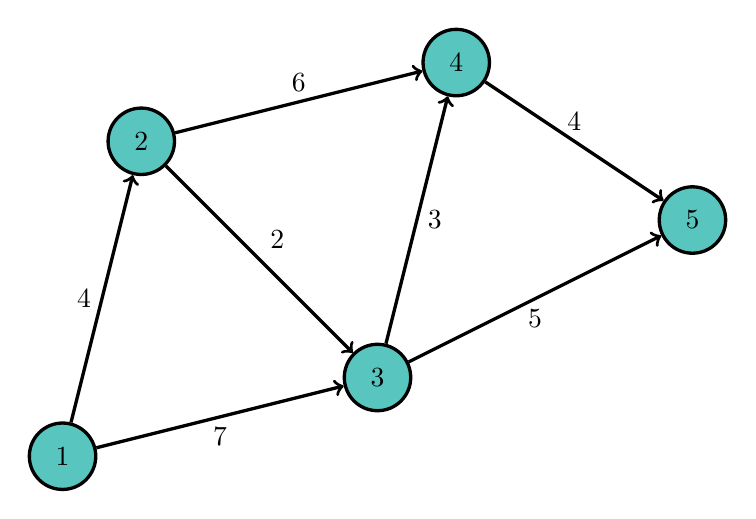
\begin{tikzpicture}[very thick,edge from parent/.style={draw,<-},level/.style={sibling distance=30mm/#1}]
\draw (0, 0) node [vertex] (v1) {1};
\draw (1, 4) node [vertex] (v2) {2};
\draw (4, 1) node [vertex] (v3) {3};
\draw (5, 5) node [vertex] (v4) {4};
\draw (8, 3) node [vertex] (v5) {5};
\draw[->] (v1) -- (v2) node[midway, left] {4};
\draw[->] (v2) -- (v3) node[midway, above right] {2};
\draw[->] (v1) -- (v3) node[midway, below] {7};
\draw[->] (v2) -- (v4) node[midway, above] {6};
\draw[->] (v3) -- (v4) node[midway, right] {3};
\draw[->] (v3) -- (v5) node[midway, below] {5};
\draw[->] (v4) -- (v5) node[midway, above] {4};
\end{tikzpicture}
\end{center}

Let's run Dijkstra's algorithm on the above graph with vertex 1 as the source. We first set all the distances besides the source to be $\infty$.

\begin{center}
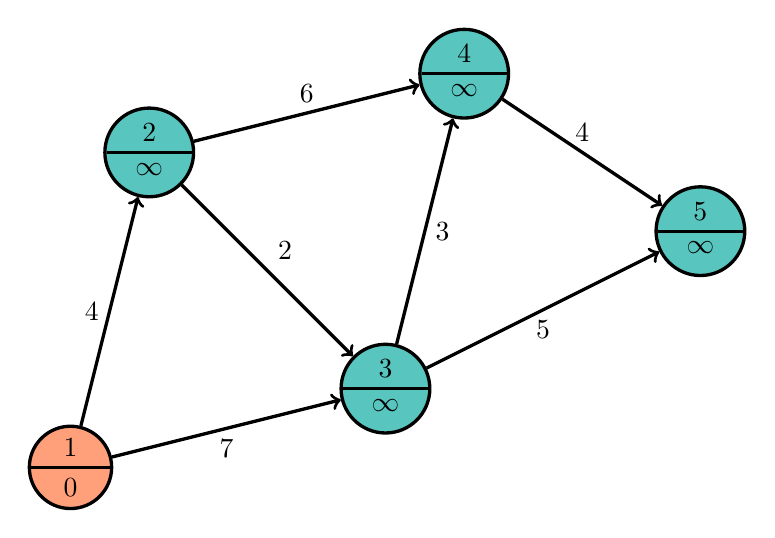
\begin{tikzpicture}[very thick,edge from parent/.style={draw,<-},level/.style={sibling distance=30mm/#1}]
\draw (0, 0) node [splitvertex, fill=mysalmon] (v1) {1\nodepart{lower}0};
\draw (1, 4) node [splitvertex] (v2) {2\nodepart{lower}$\infty$};
\draw (4, 1) node [splitvertex] (v3) {3\nodepart{lower}$\infty$};
\draw (5, 5) node [splitvertex] (v4) {4\nodepart{lower}$\infty$};
\draw (8, 3) node [splitvertex] (v5) {5\nodepart{lower}$\infty$};
\draw[->] (v1) -- (v2) node[midway, left] {4};
\draw[->] (v2) -- (v3) node[midway, above right] {2};
\draw[->] (v1) -- (v3) node[midway, below] {7};
\draw[->] (v2) -- (v4) node[midway, above] {6};
\draw[->] (v3) -- (v4) node[midway, right] {3};
\draw[->] (v3) -- (v5) node[midway, below] {5};
\draw[->] (v4) -- (v5) node[midway, above] {4};
\end{tikzpicture}
\end{center}

Now, we continue choosing the closest unvisited node, mark it as visited, and and update its neighbors.

\begin{center}
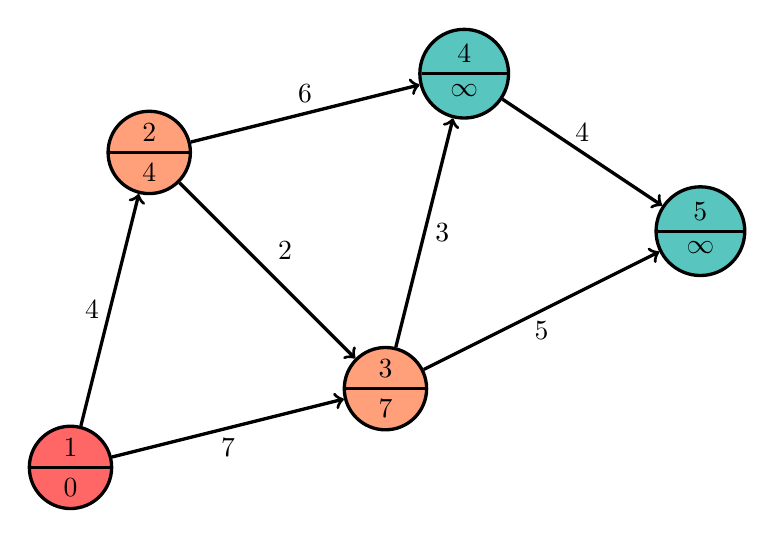
\begin{tikzpicture}[very thick,edge from parent/.style={draw,<-},level/.style={sibling distance=30mm/#1}]
\draw (0, 0) node [splitvertex, fill=myred] (v1) {1\nodepart{lower}0};
\draw (1, 4) node [splitvertex, fill=mysalmon] (v2) {2\nodepart{lower}4};
\draw (4, 1) node [splitvertex, fill=mysalmon] (v3) {3\nodepart{lower}7};
\draw (5, 5) node [splitvertex] (v4) {4\nodepart{lower}$\infty$};
\draw (8, 3) node [splitvertex] (v5) {5\nodepart{lower}$\infty$};
\draw[->] (v1) -- (v2) node[midway, left] {4};
\draw[->] (v2) -- (v3) node[midway, above right] {2};
\draw[->] (v1) -- (v3) node[midway, below] {7};
\draw[->] (v2) -- (v4) node[midway, above] {6};
\draw[->] (v3) -- (v4) node[midway, right] {3};
\draw[->] (v3) -- (v5) node[midway, below] {5};
\draw[->] (v4) -- (v5) node[midway, above] {4};
\end{tikzpicture}
\end{center}

\begin{center}
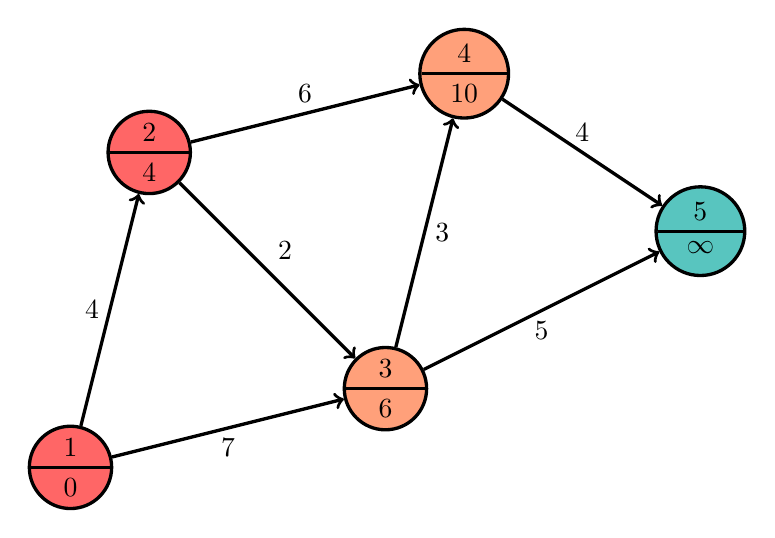
\begin{tikzpicture}[very thick,edge from parent/.style={draw,<-},level/.style={sibling distance=30mm/#1}]
\draw (0, 0) node [splitvertex, fill=myred] (v1) {1\nodepart{lower}0};
\draw (1, 4) node [splitvertex, fill=myred] (v2) {2\nodepart{lower}4};
\draw (4, 1) node [splitvertex, fill=mysalmon] (v3) {3\nodepart{lower}6};
\draw (5, 5) node [splitvertex, fill=mysalmon] (v4) {4\nodepart{lower}10};
\draw (8, 3) node [splitvertex] (v5) {5\nodepart{lower}$\infty$};
\draw[->] (v1) -- (v2) node[midway, left] {4};
\draw[->] (v2) -- (v3) node[midway, above right] {2};
\draw[->] (v1) -- (v3) node[midway, below] {7};
\draw[->] (v2) -- (v4) node[midway, above] {6};
\draw[->] (v3) -- (v4) node[midway, right] {3};
\draw[->] (v3) -- (v5) node[midway, below] {5};
\draw[->] (v4) -- (v5) node[midway, above] {4};
\end{tikzpicture}
\end{center}

\begin{center}
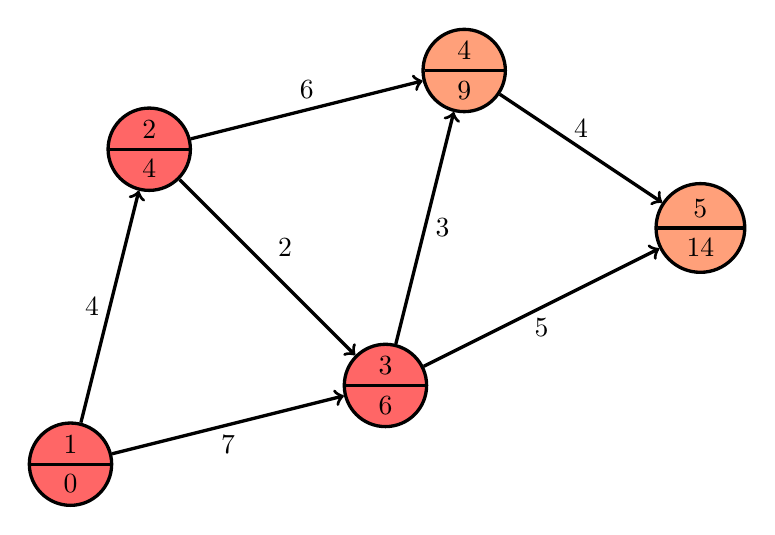
\begin{tikzpicture}[very thick,edge from parent/.style={draw,<-},level/.style={sibling distance=30mm/#1}]
\draw (0, 0) node [splitvertex, fill=myred] (v1) {1\nodepart{lower}0};
\draw (1, 4) node [splitvertex, fill=myred] (v2) {2\nodepart{lower}4};
\draw (4, 1) node [splitvertex, fill=myred] (v3) {3\nodepart{lower}6};
\draw (5, 5) node [splitvertex, fill=mysalmon] (v4) {4\nodepart{lower}9};
\draw (8, 3) node [splitvertex, fill=mysalmon] (v5) {5\nodepart{lower}14};
\draw[->] (v1) -- (v2) node[midway, left] {4};
\draw[->] (v2) -- (v3) node[midway, above right] {2};
\draw[->] (v1) -- (v3) node[midway, below] {7};
\draw[->] (v2) -- (v4) node[midway, above] {6};
\draw[->] (v3) -- (v4) node[midway, right] {3};
\draw[->] (v3) -- (v5) node[midway, below] {5};
\draw[->] (v4) -- (v5) node[midway, above] {4};
\end{tikzpicture}
\end{center}

\begin{center}
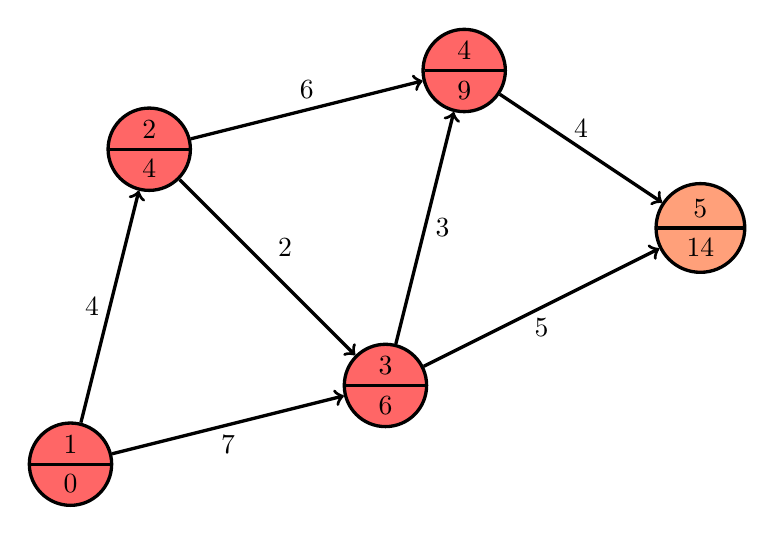
\begin{tikzpicture}[very thick,edge from parent/.style={draw,<-},level/.style={sibling distance=30mm/#1}]
\draw (0, 0) node [splitvertex, fill=myred] (v1) {1\nodepart{lower}0};
\draw (1, 4) node [splitvertex, fill=myred] (v2) {2\nodepart{lower}4};
\draw (4, 1) node [splitvertex, fill=myred] (v3) {3\nodepart{lower}6};
\draw (5, 5) node [splitvertex, fill=myred] (v4) {4\nodepart{lower}9};
\draw (8, 3) node [splitvertex, fill=mysalmon] (v5) {5\nodepart{lower}14};
\draw[->] (v1) -- (v2) node[midway, left] {4};
\draw[->] (v2) -- (v3) node[midway, above right] {2};
\draw[->] (v1) -- (v3) node[midway, below] {7};
\draw[->] (v2) -- (v4) node[midway, above] {6};
\draw[->] (v3) -- (v4) node[midway, right] {3};
\draw[->] (v3) -- (v5) node[midway, below] {5};
\draw[->] (v4) -- (v5) node[midway, above] {4};
\end{tikzpicture}
\end{center}

\begin{center}
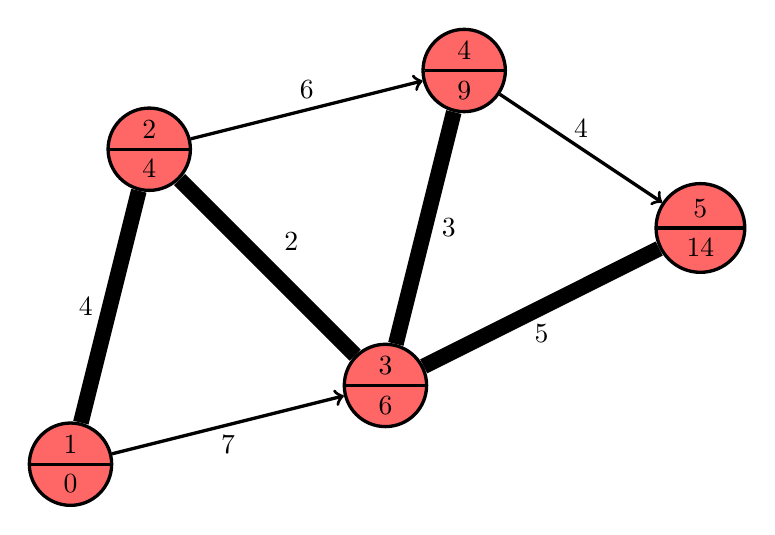
\begin{tikzpicture}[very thick,edge from parent/.style={draw,<-},level/.style={sibling distance=30mm/#1}]
\draw (0, 0) node [splitvertex, fill=myred] (v1) {1\nodepart{lower}0};
\draw (1, 4) node [splitvertex, fill=myred] (v2) {2\nodepart{lower}4};
\draw (4, 1) node [splitvertex, fill=myred] (v3) {3\nodepart{lower}6};
\draw (5, 5) node [splitvertex, fill=myred] (v4) {4\nodepart{lower}9};
\draw (8, 3) node [splitvertex, fill=myred] (v5) {5\nodepart{lower}14};
\draw[line width=2mm] (v1) -- (v2) node[midway, left] {4};
\draw[line width=2mm] (v2) -- (v3) node[midway, above right] {2};
\draw[->] (v1) -- (v3) node[midway, below] {7};
\draw[->] (v2) -- (v4) node[midway, above] {6};
\draw[line width=2mm] (v3) -- (v4) node[midway, right] {3};
\draw[line width=2mm] (v3) -- (v5) node[midway, below] {5};
\draw[->] (v4) -- (v5) node[midway, above] {4};
\end{tikzpicture}
\end{center}

The slow part of the $O(V^2)$ formulation is the linear search for the vertex $v$ with the minimum $dist(v)$. We happen to have a data structure that resolves this problem -- a binary heap. The main problem with using the standard library heap is having repeated vertices in the heap. We could just ignore this problem and discard visited vertices as they come out of the heap. Alternatively, we could choose never to have repeated vertices in the heap. To do this, we need to be able to change the value of the distances once they are already in the heap, or \textit{decrease-key}. This is a pretty simple function to add, however, if you have a heap already coded. Either way, we achieve $O(E \log{V})$, as we do $E+V$ updates to our heap, each costing $O(V)$.

\begin{enumerate}

\item
(USACO Training Pages, butter)
Farmer John owns a collection of pastures with weighted edges between some
pairs of locations. Each pasture is inhabited by a cow, and the cows wish to all congregate at one of the
pastures. Find the pasture at which the cows should meet in order to minimize combined travel distance.

\item
(USACO February 2012, relocate)
FJ is moving! He is trying to find the best place to build a new farm so as to
minimize his daily travel time.

The region to which FJ plans to move has $N$ towns ($1 \le N \le 10, 000$). There are $M$ bi-directional roads
($1 \le M \le 50, 000$) connecting certain pairs of towns. All towns are reachable from each-other via some
combination of roads. FJ needs your help selecting the best town as the home for his new farm.

There are markets in $K$ of the towns ($1 \le K \le 5$) that FJ wants to visit every day. In particular, every day
he plans to leave his new farm, visit the $K$ towns with markets, and then return to his farm. FJ can visit the
markets in any order he wishes. When selecting a town in which to build his new farm, FJ wants to choose
only from the $N - K$ towns that do not have markets, since housing prices are lower in those towns.

Please help FJ compute the minimum distance he will need to travel during his daily schedule, if he builds his
farm in an optimal location and chooses his travel schedule to the markets as smartly as possible.

\item
(USACO December 2012, mroute)
Farmer John's farm has an outdated network of $M$ pipes ($1 \le M \le 500$) for
pumping milk from the barn to his milk storage tank.  He wants to remove
and update most of these over the next year, but he wants to leave exactly
one path worth of pipes intact, so that he can still pump milk from the
barn to the storage tank.

The pipe network is described by $N$ junction points ($1 \le N \le 500$), each of
which can serve as the endpoint of a set of pipes.  Junction point 1 is the
barn, and junction point $N$ is the storage tank.  Each of the $M$
bi-directional pipes runs between a pair of junction points, and has an
associated latency (the amount of time it takes milk to reach one end of
the pipe from the other) and capacity (the amount of milk per unit time
that can be pumped through the pipe in steady state).  Multiple pipes
can connect between the same pair of junction points.

For a path of pipes connecting from the barn to the tank, the latency
of the path is the sum of the latencies of the pipes along the path,
and the capacity of the path is the minimum of the capacities of the
pipes along the path (since this is the ``bottleneck'' constraining the
overall rate at which milk can be pumped through the path).  If FJ
wants to send a total of $X$ units of milk through a path of pipes with
latency $L$ and capacity $C$, the time this takes is therefore $L + \frac{X}{C}$.

Given the structure of FJ's pipe network, please help him select a single
path from the barn to the storage tank that will allow him to pump $X$ units
of milk in a minimum amount of total time.

\item
(IOI 1999, Traffic Lights)
In the city of Dingilville the traffic is arranged in an unusual way. There are junctions
and roads connecting the junctions. There is at most one road between any two different junctions. There is no
road connecting a junction to itself. Travel time for a road is the same for both directions. At every junction
there is a single traffic light that is either blue or purple at any moment. The color of each light alternates
periodically: blue for certain duration and then purple for another duration. Traffic is permitted to travel
down the road between any two junctions, if and only if the lights at both junctions are the same color at the
moment of departing from one junction for the other. If a vehicle arrives at a junction just at the moment the
lights switch it must consider the new colors of lights. Vehicles are allowed to wait at the junctions. You are
given the city map which shows
\begin{itemize}
\item
the travel times for all roads (integers),
\item
the durations of the two colors at each junction (integers)
\item
the initial color of the light and the remaining time (integer) for this color to change at each junction.
\end{itemize}
Your task is to find a path which takes the minimum time from a given source junction to a given destination
junction for a vehicle when the traffic starts. In case more than one such path exists you are required to report
only one of them.
\end{enumerate}

\subsection{Floyd-Warshall}

Dijkstra is nice when we are dealing with edges with nonnegative weights and are looking for the distances from one vertex to all the others. Floyd-Warshall solves the shortest path problem for all pairs of vertices in $O(V^3)$ time, which is faster than $V$ single-source Dijkstra runs on a dense graph. Floyd-Warshall works even if some edge weights are negative but not if the graph has a negative cycle.

\begin{algorithm}[H]
\caption{Floyd-Warshall}
\begin{algorithmic}
\ForAll{vertices $v$}
	\State $dist(v,v)=0$
\EndFor
\ForAll{edges $(u,v)$}
	\State $dist(u,v)=weight(u,v)$
\EndFor
\ForAll{vertices $k$}
	\ForAll{vertices $i$}
    	\ForAll{vertices $j$}
        	\If{$dist(i,j) > dist(i,k)+dist(k,j)$}
            	\State $dist(i,j) \gets dist(i,k)+dist(k,j)$
            \EndIf
        \EndFor
    \EndFor
\EndFor
\end{algorithmic}
\end{algorithm}

\subsection{Bellman-Ford}

Bellman-Ford is a single-source $O(VE)$ shortest path algorithm that works when edge weights can be negative. It is preferable to Floyd-Warshall when the graph is sparse and we only need the answer for one source. Like Floyd-Warshall, the algorithm fails if the graph contains a negative cycle, but the algorithm is still useful for detecting negative cycles.

The idea here is the shortest path, assuming no negative cycles, has length at most $V-1$.

\begin{algorithm}[H]
\caption{Bellman-Ford}
\begin{algorithmic}
\ForAll{vertices $v$}
	\State $dist(v)\gets\infty$
    \State $prev(v)=\gets -1$
\EndFor
\State $dist(src) \gets 0$
\For{$i\equiv 1,V-1$}
	\ForAll{edges $(u,v)$}
		\If{$dist(u)+weight(u,v) < dist(v)$}
    	    \State $dist(v) \gets dist(u)+weight(u,v)$
	        \State $prev(v) \gets u$
        \EndIf
	\EndFor
\EndFor
\ForAll{edges $(u,v)$}
	\Comment{check for negative cycles}
	\If{$dist(u)+weight(u,v) < dist(v)$}
   	    \State{negative cycle detected}
	\EndIf
\EndFor
\end{algorithmic}
\end{algorithm}

\section{Minimum Spanning Tree}

Consider a connected, undirected graph. A \textit{spanning tree} is a subgraph that is a tree and contains every vertex in the original graph. A \textit{minimum spanning tree} is a spanning tree such that the sum of the edge weights of the tree is minimized. Finding the minimum spanning tree uses many of the same ideas discussed earlier.

\begin{center}
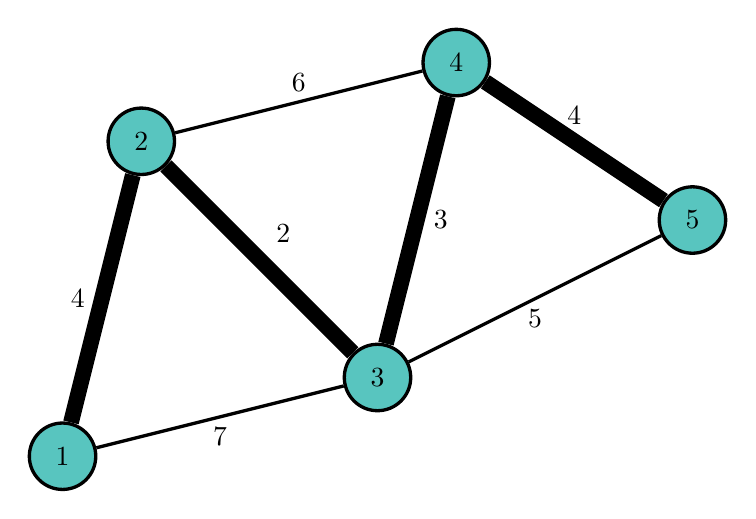
\begin{tikzpicture}[very thick,edge from parent/.style={draw,<-},level/.style={sibling distance=30mm/#1}]
\draw (0, 0) node [vertex] (v1) {1};
\draw (1, 4) node [vertex] (v2) {2};
\draw (4, 1) node [vertex] (v3) {3};
\draw (5, 5) node [vertex] (v4) {4};
\draw (8, 3) node [vertex] (v5) {5};
\draw[line width=2mm] (v1) -- (v2) node[midway, left] {4};
\draw[line width=2mm] (v2) -- (v3) node[midway, above right] {2};
\draw (v1) -- (v3) node[midway, below] {7};
\draw (v2) -- (v4) node[midway, above] {6};
\draw[line width=2mm] (v3) -- (v4) node[midway, right] {3};
\draw (v3) -- (v5) node[midway, below] {5};
\draw[line width=2mm] (v4) -- (v5) node[midway, above] {4};
\end{tikzpicture}
\end{center}

\subsection{Prim}

Prim's algorithm for finding the minimum spanning tree is very similar to Dijkstra's algorithm for finding the shortest path. Like Dijkstra, it iteratively adds a new vertex at a time to build a tree. The only difference is $dist(v)$ stores the shortest distance from \textit{any} visited node instead of the source.

\begin{algorithm}[H]
\caption{Prim}
\begin{algorithmic}
\ForAll{vertices $v$}
	\State $dist(v) \gets \infty$
	\State $visited(v) \gets 0$
    \State $prev(v) \gets -1$
\EndFor
\State $dist(src) \gets 0$
\While{$\exists v$ s.t. $visited(v)=0$}
	\State $v \equiv v$ s.t. $visited(v)=0$ with min $dist(v)$
    \State $visited(v) \gets 1$
	\ForAll{neighbors $u$ of $v$}
    	\If{$visited(u) = 0$}
			\If{$weight(v, u) < dist(u)$}
				\State $dist(u) \gets weight(v, u)$
   	        	\State $prev(u) \gets v$
			\EndIf
        \EndIf
    \EndFor
\EndWhile
\end{algorithmic}
\end{algorithm}

The proof of correctness is left as an exercise. The complexity of this algorithm depends on how the minimum unvisited vertex is calculated. Using the same approaches as Dijkstra, we can achieve $O(V^2)$ or $O(E \log{V})$.

\begin{enumerate}

\item
(USACO March 2014, irrigation)
Due to a lack of rain, Farmer John wants to build an irrigation system to
send water between his $N$ fields ($1 \le N \le 2000$).

Each field $i$ is described by a distinct point $(x_i, y_i)$ in the 2D plane,
with 0 <= xi, yi <= 1000.  The cost of building a water pipe between two
fields $i$ and $j$ is equal to the squared Euclidean distance between them: 

\[(x_i - x_j)^2 + (y_i - y_j)^2\]

FJ would like to build a minimum-cost system of pipes so that all of his
fields are linked together -- so that water in any field can follow a
sequence of pipes to reach any other field.  

Unfortunately, the contractor who is helping FJ install his irrigation
system refuses to install any pipe unless its cost (squared Euclidean
length) is at least $C$ ($1 \le C \le 1,000,000$).  

Please help FJ compute the minimum amount he will need pay to connect all
his fields with a network of pipes.

\item
(USACO February 2015, superbull)
Bessie and her friends are playing hoofball in the annual Superbull championship, and Farmer John is in charge of making the tournament as exciting as possible. A total of $N$ ($1 \le N \le 2000$) teams are playing in the Superbull. Each team is assigned a distinct integer team ID in the range $[1,2^{30}-1]$ to distinguish it from the other teams. The Superbull is an elimination tournament -- after every game, Farmer John chooses which team to eliminate from the Superbull, and the eliminated team can no longer play in any more games. The Superbull ends when only one team remains.

Farmer John notices a very unusual property about the scores in matches! In any game, the combined score of the two teams always ends up being the bitwise exclusive OR ($XOR$) of the two team IDs. For example, if teams 12 and 20 were to play, then 24 points would be scored in that game, since $01100 XOR 10100 = 11000$.

Farmer John believes that the more points are scored in a game, the more exciting the game is. Because of this, he wants to choose a series of games to be played such that the total number of points scored in the Superbull is maximized. Please help Farmer John organize the matches.

\end{enumerate}

\subsection{Kruskal}

While Prim greedily adds vertices to the tree, Kruskal's algorithm greedily adds edges. It iterates over all the edges, sorted by weight. We need to watch out for adding a cycle, breaking the tree structure, which means we need to keep track of each vertex's connected component. If an edge connects two vertices from the same connected component, we don't want to add it to our tree. However, we have a union-find algorithm that works perfectly for this.

\begin{algorithm}[H]
\caption{Kruskal}
\begin{algorithmic}
\ForAll{edges $(u,v)$ in sorted order}
	\If{$\Call{Find}{u} \not= \Call{Find}{v}$}
		\State add $(u,v)$ to spanning tree
		\State $\Call{Union}{u,v}$
	\EndIf
\EndFor
\end{algorithmic}
\end{algorithm}

This algorithm requires a sort of the edges and thus has complexity $O(E \log{E}) = O(E \log{V})$.

\begin{enumerate}
\item
(SPOJ, INVENT)
Given tree with $N$ ($1 \le N \le 15,000$) vertices, find the minimum possible weight of a complete
graph (a graph where every pair of vertices is connected) such that the given tree is its unique minimum spanning
tree.
\end{enumerate}

\section{Eulerian Tour}

An \textit{Eulerian tour} of a graph is a path that traverses every edge exactly once. If the tour ends exactly where it started, it is called an \textit{Eulerian circuit}. A graph has an Eulerian circuit if it is connected and every vertex has even degree. A graph has an Eulerian path if it is connected and all vertices but exactly two have even degrees. The mathematical proofs for these graph properties hinge on the idea that removing a cycle from the graph maintains the Eulerian property. We construct an Eulerian tour by appealing to this idea.

\begin{algorithm}
\caption{Eulerian Tour}
\begin{algorithmic}
\Function{FindTour}{$v$}
\While{$v$ has a neighbor $u$}
	\State delete edge $(v,u)$
	\State \Call{FindTour}{$u$}
	\Comment{\Call{FindTour}{$u$} must trace a circuit back to $v$}
\EndWhile
\State add $v$ to tour
\EndFunction
\end{algorithmic}
\end{algorithm}

It is not preferable to use the run-time stack; we can use our own stack if necessary.

If the graph contains an Eulerian circuit, we call this function on any vertex we like. If it contains an Eulerian path, we call this function on one of the vertices with odd degree.

\begin{enumerate}

\item
(USACO Training, Airplane Hopping)
Given a collection of cities, along with the flights between those cities, determine if there is a sequence of flights such that you take every flight exactly once, and end up at the place you started. (In other words, find an Eulerian circuit on a directed graph.)

\item
(USACO Training, Cows on Parade)
Farmer John has two types of cows: black Angus and white Jerseys. While marching 19 of their cows to market the other day, John's wife Farmeress Joanne, noticed that all 16 possibilities of four successive black and white cows (e.g., $bbbb$, $bbbw$, $bbwb$, $bbww$, \ldots, $wwww$) were present. Of course, some of the combinations overlapped others.

Given $N$ ($2 \le N \le 15$), find the minimum length sequence of cows such that every combination of $N$ successive black and white cows occurs in that sequence.

(The answer is not hard to guess, but use Eulerian circuits to prove that it is correct.)

\end{enumerate}

\section{Maximum Flow}

We are given a directed connected graph with weighted edges, a source node, and a sink node. Each edge weight represents the maximum capacity of that edge in the ``flow." For every node besides the source and the sink node, total flow in is equal to total flow out. Our goal is to maximize total flow from source to sink.

A natural approach to ``solving'' this problem would be to use the greedy algorithm:

Find a path from the source to the sink with the maximum flow; that is, the path with the largest capacity of the minimum of the edges along this path. ``Send flow" along this path from the source to the sink by decreasing each edge along this path by the capacity of the path. We repeat, and this is guaranteed to terminate since on any given move, we ``remove" an edge.

What is wrong with our greedy approach? Consider the following graph:

\begin{center}
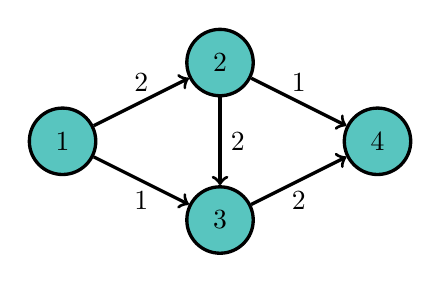
\begin{tikzpicture}[very thick,level/.style={sibling distance=70mm/#1}]
\draw (0, 0) node [vertex] (n1) {1};
\draw (2, 1) node [vertex] (n2) {2};
\draw (2, -1) node  [vertex] (n3) {3};
\draw (4, 0) node [vertex] (n4) {4};
\draw[->] (n1) -- (n2) node[midway, above] {2};
\draw[->] (n2) -- (n3) node[midway, right] {2};
\draw[->] (n3) -- (n4) node[midway, below] {2};
\draw[->] (n2) -- (n4) node[midway, above] {1};
\draw[->] (n1) -- (n3) node[midway, below] {1};
\end{tikzpicture}
\end{center}

The max flow from vertex 1 to vertex 4 is 3, but greedy gives only 2.

\subsection{Ford-Fulkerson}

Find a path from the source to the sink in which all the edges have positive weight. Find the max flow across this path, which is the minimum weight of any edge on this particular path. Call this value $cap$. Then subtract $cap$ from the weight of every edge along the path and \textit{increment the reverse edge} (the edge connecting the same two vertices but running in the opposite direction) by $cap$.

The difference between this algorithm and the greedy approach from earlier is that the paths we now allow may run along a reverse path, essentially undoing any suboptimal flow from earlier. These more general paths are called \textit{augmenting paths}.

This algorithm is guaranteed to terminate for graphs with integral weights. However, it is not guaranteed to terminate for graphs with non-integral capacities. For graphs with integral weights, the run time is $O(Ef)$, where $f$ is the maximum flow and $E$ is the number of edges. In practice, run time tends to be much faster since the algorithm still greedily adds the most flow it can at each step.

\subsection{Edmonds-Karp}

Edmonds-Karp is a slight refinement of Ford-Fulkerson.

\subsection{Push-Relabel}

\subsection{Max-Flow Min-Cut}

\chapter{Computational Geometry}

For actual geometry problems, and not graph theory problems hiding in the plane.

I'm too lazy to actually write this section right now so here are some useful links from the USACO Training Pages.

\url{https://www.dropbox.com/s/nqzk63bjby1iaq9/Computational%20Geometry.pdf?dl=0}

\url{https://www.dropbox.com/s/ykf65dk6sefb6zk/2-D%20Convex%20Hull.pdf?dl=0}

These essentially cover anything I would want to say in this chapter anyway, so I'll likely fill this chapter out last.

\section{Basic Tools}

\subsubsection{Cross Product}

\subsubsection{Dot Product}

\subsubsection{$\tan^{-1}$, \texttt{atan2}}

\section{Formulas}

\subsection{Area}

\subsection{Distance}

\subsection{Configuration}

\subsection{Intersection}

\section{Convex Hull}

\chapter{Strings}

\section{Rabin-Karp}

\section{Knuth-Morris-Pratt}

\url{https://activities.tjhsst.edu/sct/lectures/1415/stringmatching_10_3_14.pdf}

\section{Aho-Corasick}

\section{Trie}

\section{Suffix Tree}

\section{Suffix Array}

\chapter{More Stuff}

Here are some more tools to stuff in the toolbox. This chapter introduces more complex ideas that are useful for solving USACO Gold problems and beyond.

\section{$\sqrt{n}$ Bucketing}

$\sqrt{n}$ bucketing is a relatively straightforward idea -- given $n$ elements $\{a_i\}_{i=1}^n$ in a sequence, we group them into $\sqrt{n}$ equal-sized buckets. The motivation for arranging elements like this is to support an operation called a \textit{range query}.

Let's take a concrete example. Suppose we want to support two operations:

\begin{itemize}
\item
$update(i, x)$ -- increment the value of $a_i$ by $x$

\item
$query(i, j)$ -- return $\sum_{k=i}^j a_k$.
\end{itemize}

Suppose we simply stored the sequence in an array. $update$ then becomes an $O(1)$ operation, but $query$ is $O(n)$.

\begin{center}
{
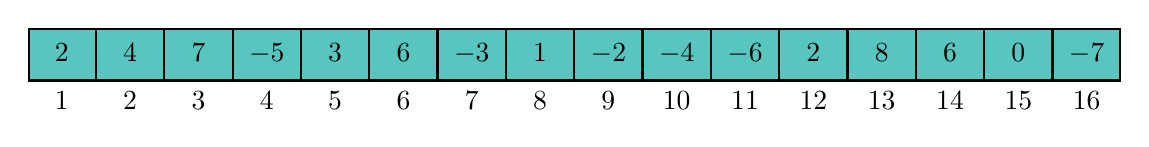
\begin{tikzpicture}[
  thick,
  myrect/.style={
    draw,
    fill=myseagreen,
    rectangle split,
    rectangle split horizontal,
    rectangle split parts=#1,
    rectangle split part align=left,
    text width=4ex,
    text centered
    }
]

\node[myrect=16]
  (array)
  {
  					\strut 2
  \nodepart{two}	\strut 4
  \nodepart{three}	\strut 7
  \nodepart{four}	\strut $-5$
  \nodepart{five}	\strut 3
  \nodepart{six}	\strut 6
  \nodepart{seven}	\strut $-3$
  \nodepart{eight}	\strut 1
  \nodepart{nine}	\strut $-2$
  \nodepart{ten}	\strut $-4$
  \nodepart{eleven}	\strut $-6$
  \nodepart{twelve}	\strut 2
  \nodepart{thirteen}	\strut 8
  \nodepart{fourteen}	\strut 6
  \nodepart{fifteen}	\strut 0
  \nodepart{sixteen}	\strut $-7$
  };
\foreach \Valor [count=\Valori from 1] in {one ,two ,three , four , five , six , seven , eight , nine , ten , eleven , twelve , thirteen , fourteen , fifteen , sixteen }
  \node[below] at (array.\Valor south) {\Valori};

\end{tikzpicture}
}
\end{center}

Another natural approach would be to store in a separate array the sum of the first $i$ terms in the sequence for every index $i$, or store the \textit{prefix sums}.

\begin{center}
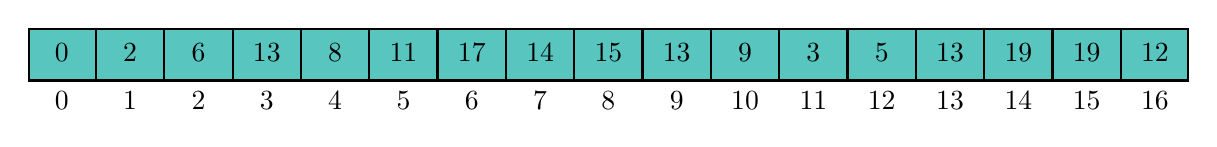
\begin{tikzpicture}[
  thick,
  myrect/.style={
    draw,
    fill=myseagreen,
    rectangle split,
    rectangle split horizontal,
    rectangle split parts=#1,
    rectangle split part align=left,
    text width=4ex,
    text centered
    }
]

\node[myrect=17]
  (array)
  {
  					\strut 0
  \nodepart{two}	\strut 2
  \nodepart{three}	\strut 6
  \nodepart{four}	\strut 13
  \nodepart{five}	\strut 8
  \nodepart{six}	\strut 11
  \nodepart{seven}	\strut 17
  \nodepart{eight}	\strut 14
  \nodepart{nine}	\strut 15
  \nodepart{ten}	\strut 13
  \nodepart{eleven}	\strut 9
  \nodepart{twelve}	\strut 3
  \nodepart{thirteen}	\strut 5
  \nodepart{fourteen}	\strut 13
  \nodepart{fifteen}	\strut 19
  \nodepart{sixteen}	\strut 19
  \nodepart{seventeen}	\strut 12
  };
\foreach \Valor [count=\Valori from 0] in {one ,two ,three , four , five , six , seven , eight , nine , ten , eleven , twelve , thirteen , fourteen , fifteen , sixteen , seventeen }
  \node[below] at (array.\Valor south) {\Valori};

\end{tikzpicture}

\end{center}

Now $query$ becomes an $O(1)$ operation, as we can simply subtract two elements in the array to answer a query. Unfortunately, $update$ becomes $O(n)$, as changing the value of an element in the beginning of the sequence forces us to change almost all the values in the prefix sum array.

We can still use this idea, though... what we are looking for is some way to group values into sums such that we only need to change a small number of the sums to $update$ and only require a small number of them to $query$.

This leads us directly to a $\sqrt{n}$ bucketing solution. Let's group the 16 elements into 4 groups.

\begin{center}
{
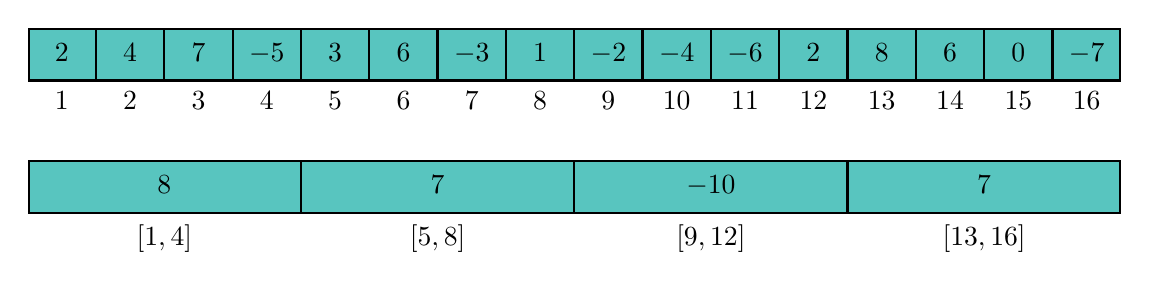
\begin{tikzpicture}[
  thick,
  myrect/.style={
    draw,
    fill=myseagreen,
    rectangle split,
    rectangle split horizontal,
    rectangle split parts=#1,
    rectangle split part align=left,
    text width=4ex,
    text centered
    }
]

\node[myrect=16]
  (array2)
  {
  					\strut 2
  \nodepart{two}	\strut 4
  \nodepart{three}	\strut 7
  \nodepart{four}	\strut $-5$
  \nodepart{five}	\strut 3
  \nodepart{six}	\strut 6
  \nodepart{seven}	\strut $-3$
  \nodepart{eight}	\strut 1
  \nodepart{nine}	\strut $-2$
  \nodepart{ten}	\strut $-4$
  \nodepart{eleven}	\strut $-6$
  \nodepart{twelve}	\strut 2
  \nodepart{thirteen}	\strut 8
  \nodepart{fourteen}	\strut 6
  \nodepart{fifteen}	\strut 0
  \nodepart{sixteen}	\strut $-7$
  };
\foreach \Valor [count=\Valori from 1] in {one ,two ,three , four , five , six , seven , eight , nine , ten , eleven , twelve , thirteen , fourteen , fifteen , sixteen }
  \node[below] at (array2.\Valor south) {\Valori};

\node[myrect=4, text width=21.2ex] [below=of array2]
  (array)
  {
  					\strut 8
  \nodepart{two}	\strut 7
  \nodepart{three}	\strut $-10$
  \nodepart{four}	\strut 7
  };

\node[below] at (array.one south) {$[1,4]$};
\node[below] at (array.two south) {$[5,8]$};
\node[below] at (array.three south) {$[9,12]$};
\node[below] at (array.four south) {$[13,16]$};
\end{tikzpicture}
}
\end{center}

We'll keep track of the total sum of each group. Now, if we want to update a value, we need to change only two values -- the value of that element in the original array and the total sum of the bucket it is in. When we query a range, we'll take advantage of the sum of the bucket when we can. Highlighted are the numbers we'll need for $query(7,15)$.

\begin{center}
{
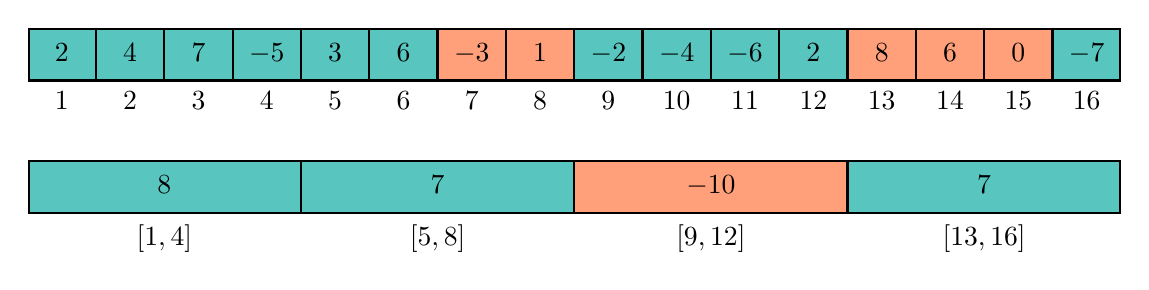
\begin{tikzpicture}[
  thick,
  myrect/.style={
    draw,
    rectangle split,
    rectangle split horizontal,
    rectangle split parts=#1,
    rectangle split part align=left,
    text width=4ex,
    text centered
    }
]

\node[myrect=16, rectangle split part fill={myseagreen, myseagreen, myseagreen, myseagreen, myseagreen, myseagreen, mysalmon, mysalmon, myseagreen, myseagreen, myseagreen, myseagreen, mysalmon, mysalmon, mysalmon, myseagreen}]
  (array2)
  {
  					\strut 2
  \nodepart{two}	\strut 4
  \nodepart{three}	\strut 7
  \nodepart{four}	\strut $-5$
  \nodepart{five}	\strut 3
  \nodepart{six}	\strut 6
  \nodepart{seven}	\strut $-3$
  \nodepart{eight}	\strut 1
  \nodepart{nine}	\strut $-2$
  \nodepart{ten}	\strut $-4$
  \nodepart{eleven}	\strut $-6$
  \nodepart{twelve}	\strut 2
  \nodepart{thirteen}	\strut 8
  \nodepart{fourteen}	\strut 6
  \nodepart{fifteen}	\strut 0
  \nodepart{sixteen}	\strut $-7$
  };
\foreach \Valor [count=\Valori from 1] in {one ,two ,three , four , five , six , seven , eight , nine , ten , eleven , twelve , thirteen , fourteen , fifteen , sixteen }
  \node[below] at (array2.\Valor south) {\Valori};

\node[myrect=4, text width=21.2ex, rectangle split part fill={myseagreen, myseagreen, mysalmon, myseagreen}] [below=of array2]
  (array)
  {
  					\strut 8
  \nodepart{two}	\strut 7
  \nodepart{three}	\strut $-10$
  \nodepart{four}	\strut 7
  };

\node[below] at (array.one south) {$[1,4]$};
\node[below] at (array.two south) {$[5,8]$};
\node[below] at (array.three south) {$[9,12]$};
\node[below] at (array.four south) {$[13,16]$};

\end{tikzpicture}
}
\end{center}

Querying requires access to at most $\sqrt{n}$ bucket sums and $2(\sqrt{n}-1)$ individual values. Therefore we have $O(\sqrt{n})$ query and $O(1)$ update. We are able to improve $O(\sqrt{n})$ update to $O(1)$ because of nice properties of the $+$ operator. This is not always the case for range queries: suppose, for instance, we needed to find the minimum element on a range.

It is often the case that $O(\sqrt{n})$ bounds can be improved to $O(\log{n})$ using more complex data structures like segment trees and more complex ideas like $2^n$ jump pointers, both of which are covered in this chapter. These are, however, more complicated to implement and as such are often comparable in runtime in the contest environment. Steven Hao is notorious for using crude $\sqrt{n}$ bucketing algorithms to solve problems that should have required tighter algorithm complexities. $\sqrt{n}$ bucketing is a crude yet powerful idea; always keep it in the back of your mind.

\section{Segment Tree}

It turns out for our specific sum problem that we can do as good as $O(\log{n})$ with a \textit{segment tree}, or \textit{range tree}, or \textit{augmented static BBST}. The essential idea is still the same -- we want to group elements in some way that allows us to update and query efficiently.

As the name ``tree'' suggests, we draw inspiration from a binary structure. Let's build a tree on top of the array, where each node keeps track of the sum of the numbers associated with its children.

\begin{center}
{
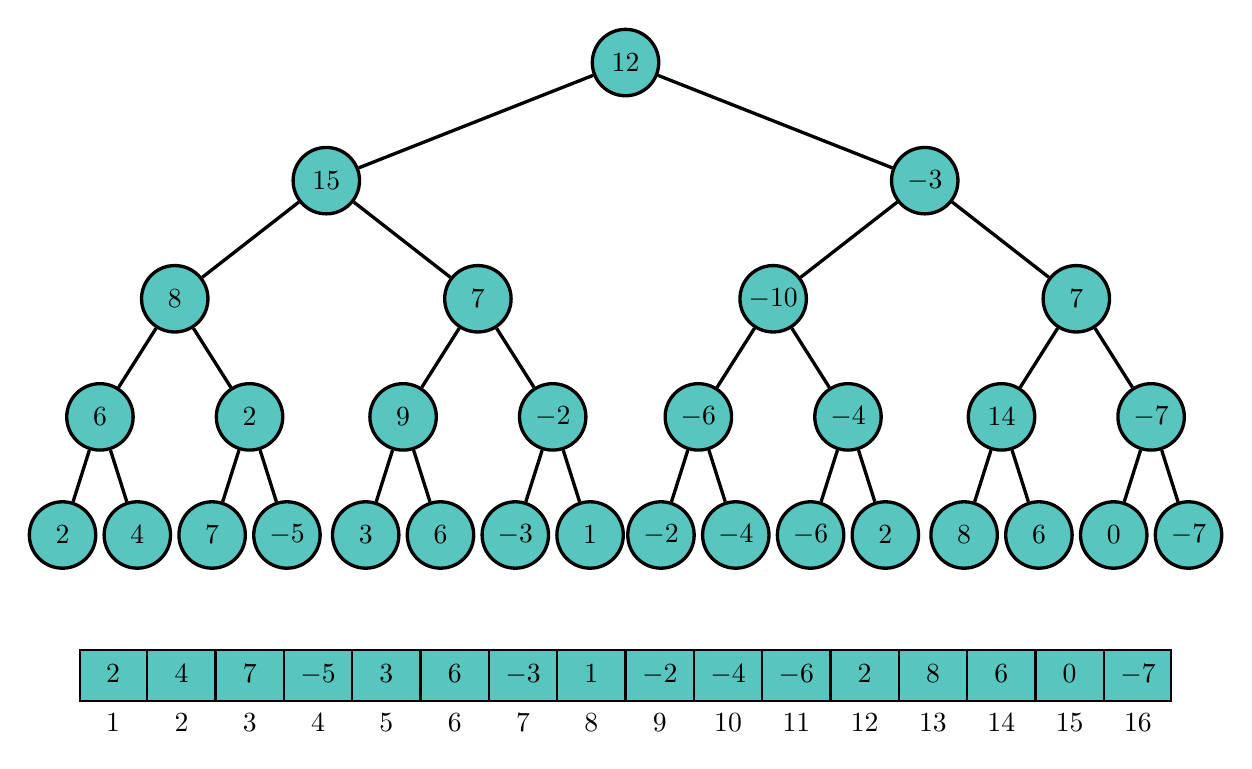
\begin{tikzpicture}[
  very thick,
  level 1/.style={sibling distance=76mm},
  level 2/.style={sibling distance=38.5mm},
  level 3/.style={sibling distance=19mm},
  level 4/.style={sibling distance=9.5mm},
  myrect/.style={
    draw,
    thick,
    fill=myseagreen,
    rectangle split,
    rectangle split horizontal,
    rectangle split parts=#1,
    rectangle split part align=left,
    text width=4ex,
    text centered
    }
]
\node [vertex] (r){$12$}
  child {
    node [vertex] (a) {15}
    child {
      node [vertex] {8}
      child {
        node [vertex] {6}
        child {node [vertex] {2}}
        child {node [vertex] {4}}
      } 
      child {
        node [vertex] {2}
        child {node [vertex] {7}}
        child {node [vertex] {$-5$}}
      }
    }
    child {
      node [vertex] {7}
      child {node [vertex] {9}
              child {node [vertex] {3}}
        child {node [vertex] {6}}
      }
      child {node [vertex] {$-2$}
              child {node [vertex] {$-3$}}
        child {node [vertex] {1}}
      }
    }
  }
  child {
    node [vertex] {$-3$}
    child {
      node [vertex] {$-10$}
      child {node [vertex] {$-6$}
              child {node [vertex] {$-2$}}
        child {node [vertex] {$-4$}}}
      child {node [vertex] {$-4$}
              child {node [vertex] {$-6$}}
        child {node [vertex] {$2$}}}
    }
    child {
      node [vertex] {7}
      child {node [vertex] {14}
              child {node [vertex] {8}}
        child {node [vertex] {6}}}
      child {node [vertex] {$-7$}
              child {node [vertex] {0}}
        child {node [vertex] {$-7$}}}
    }
  };

\node[myrect=16] [below=7cm of r]
  (array)
  {
  					\strut 2
  \nodepart{two}	\strut 4
  \nodepart{three}	\strut 7
  \nodepart{four}	\strut $-5$
  \nodepart{five}	\strut 3
  \nodepart{six}	\strut 6
  \nodepart{seven}	\strut $-3$
  \nodepart{eight}	\strut 1
  \nodepart{nine}	\strut $-2$
  \nodepart{ten}	\strut $-4$
  \nodepart{eleven}	\strut $-6$
  \nodepart{twelve}	\strut 2
  \nodepart{thirteen}	\strut 8
  \nodepart{fourteen}	\strut 6
  \nodepart{fifteen}	\strut 0
  \nodepart{sixteen}	\strut $-7$
  };
\foreach \Valor [count=\Valori from 1] in {one ,two ,three , four , five , six , seven , eight , nine , ten , eleven , twelve , thirteen , fourteen , fifteen , sixteen }
  \node[below] at (array.\Valor south) {\Valori};

\end{tikzpicture}
}
\end{center}

Highlighted are the nodes we'll need to access for $query(7,15)$. Notice how the subtrees associated with each of these nodes neatly covers the entire range $[7,15]$.

\begin{center}
{
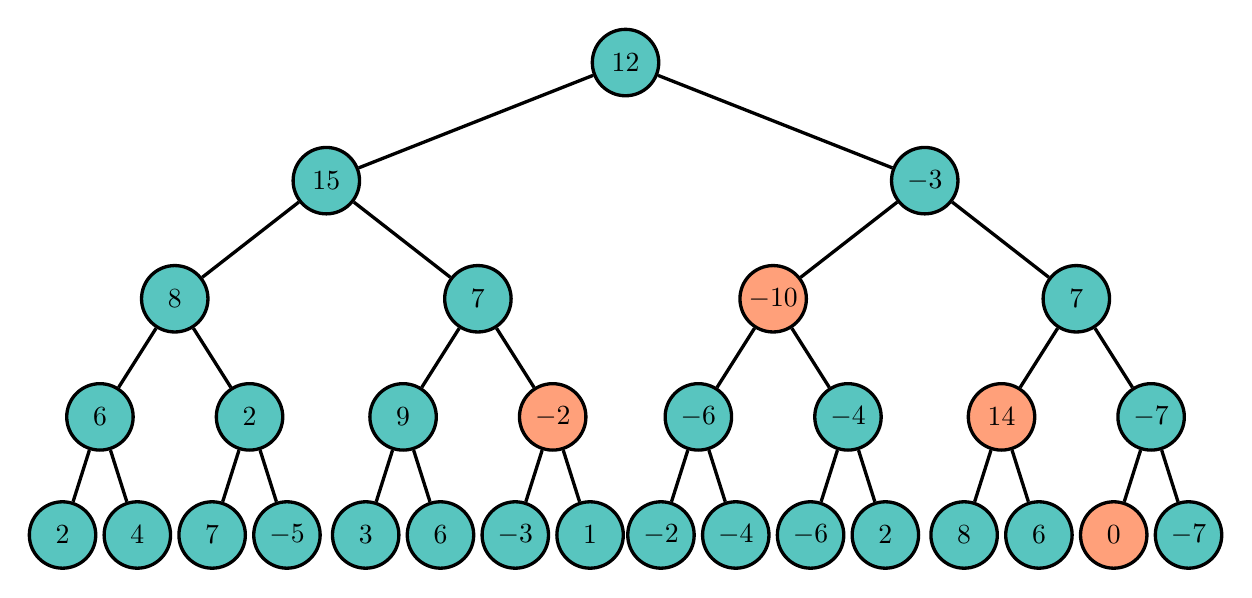
\begin{tikzpicture}[
  very thick,
  level 1/.style={sibling distance=76mm},
  level 2/.style={sibling distance=38.5mm},
  level 3/.style={sibling distance=19mm},
  level 4/.style={sibling distance=9.5mm},
  myrect/.style={
    draw,
    thick,
    fill=myseagreen,
    rectangle split,
    rectangle split horizontal,
    rectangle split parts=#1,
    rectangle split part align=left,
    text width=4ex,
    text centered
    }
]
\node [vertex] (r){$12$}
  child {
    node [vertex] (a) {15}
    child {
      node [vertex] {8}
      child {
        node [vertex] {6}
        child {node [vertex] {2}}
        child {node [vertex] {4}}
      } 
      child {
        node [vertex] {2}
        child {node [vertex] {7}}
        child {node [vertex] {$-5$}}
      }
    }
    child {
      node [vertex] {7}
      child {node [vertex] {9}
              child {node [vertex] {3}}
        child {node [vertex] {6}}
      }
      child {node [vertex, fill=mysalmon] {$-2$}
              child {node [vertex] {$-3$}}
        child {node [vertex] {1}}
      }
    }
  }
  child {
    node [vertex] {$-3$}
    child {
      node [vertex, fill=mysalmon] {$-10$}
      child {node [vertex] {$-6$}
              child {node [vertex] {$-2$}}
        child {node [vertex] {$-4$}}}
      child {node [vertex] {$-4$}
              child {node [vertex] {$-6$}}
        child {node [vertex] {$2$}}}
    }
    child {
      node [vertex] {7}
      child {node [vertex, fill=mysalmon] {14}
              child {node [vertex] {8}}
        child {node [vertex] {6}}}
      child {node [vertex] {$-7$}
              child {node [vertex, fill=mysalmon] {0}}
        child {node [vertex] {$-7$}}}
    }
  };

\end{tikzpicture}
}
\end{center}

Again, the key idea is if the the interval associated with a node is completely contained within the interval we are querying, we simply return the sum associated with that node. Otherwise, we recurse on the two children. This process is $O(\log{n})$ because each level in the tree can have at most two highlighted nodes.

If we wanted to change the third element to 2, we would have to update the highlighted nodes in the following diagram. This process is more straightforward than the querying.

\begin{center}
{
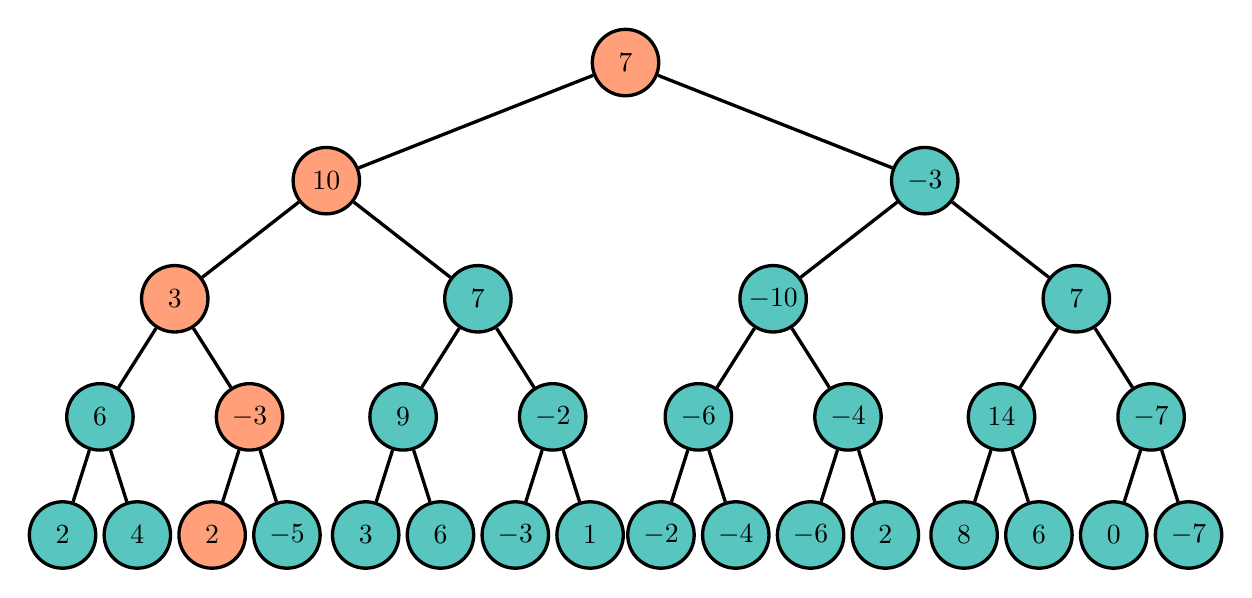
\begin{tikzpicture}[
  very thick,
  level 1/.style={sibling distance=76mm},
  level 2/.style={sibling distance=38.5mm},
  level 3/.style={sibling distance=19mm},
  level 4/.style={sibling distance=9.5mm},
  myrect/.style={
    draw,
    thick,
    fill=myseagreen,
    rectangle split,
    rectangle split horizontal,
    rectangle split parts=#1,
    rectangle split part align=left,
    text width=4ex,
    text centered
    }
]
\node [vertex, fill=mysalmon] (r){7}
  child {
    node [vertex, fill=mysalmon] (a) {10}
    child {
      node [vertex, fill=mysalmon] {3}
      child {
        node [vertex] {6}
        child {node [vertex] {2}}
        child {node [vertex] {4}}
      } 
      child {
        node [vertex, fill=mysalmon] {$-3$}
        child {node [vertex, fill=mysalmon] {2}}
        child {node [vertex] {$-5$}}
      }
    }
    child {
      node [vertex] {7}
      child {node [vertex] {9}
              child {node [vertex] {3}}
        child {node [vertex] {6}}
      }
      child {node [vertex] {$-2$}
              child {node [vertex] {$-3$}}
        child {node [vertex] {1}}
      }
    }
  }
  child {
    node [vertex] {$-3$}
    child {
      node [vertex] {$-10$}
      child {node [vertex] {$-6$}
              child {node [vertex] {$-2$}}
        child {node [vertex] {$-4$}}}
      child {node [vertex] {$-4$}
              child {node [vertex] {$-6$}}
        child {node [vertex] {$2$}}}
    }
    child {
      node [vertex] {7}
      child {node [vertex] {14}
              child {node [vertex] {8}}
        child {node [vertex] {6}}}
      child {node [vertex] {$-7$}
              child {node [vertex] {0}}
        child {node [vertex] {$-7$}}}
    }
  };

\end{tikzpicture}
}
\end{center}

Updating is also $O(\log{n})$ as we need to change the values of at most one node in each level in the tree.

I cheated with my example by using a nice power of two, $n=16$, as the number of elements in the sequence. Of course, the size is not always this nice. One solution is to simply pad the back of the sequence with enough 0s and pretend that the number of elements in the sequence is actually a power of two. For the segment tree, this is not necessary -- if a vertex is associated with the range $[a,b]$, we can simply split this range into two,
$\left[a,\floor{\frac{a+b-1}{2}}\right]$ and $\left[\floor{\frac{a+b-1}{2}}+1,b\right]$. We then recursively apply this pattern except for when the lower bound of the range is equal to the upper bound. If $n=12$, the resulting tree would have the following structure.

\begin{center}
{
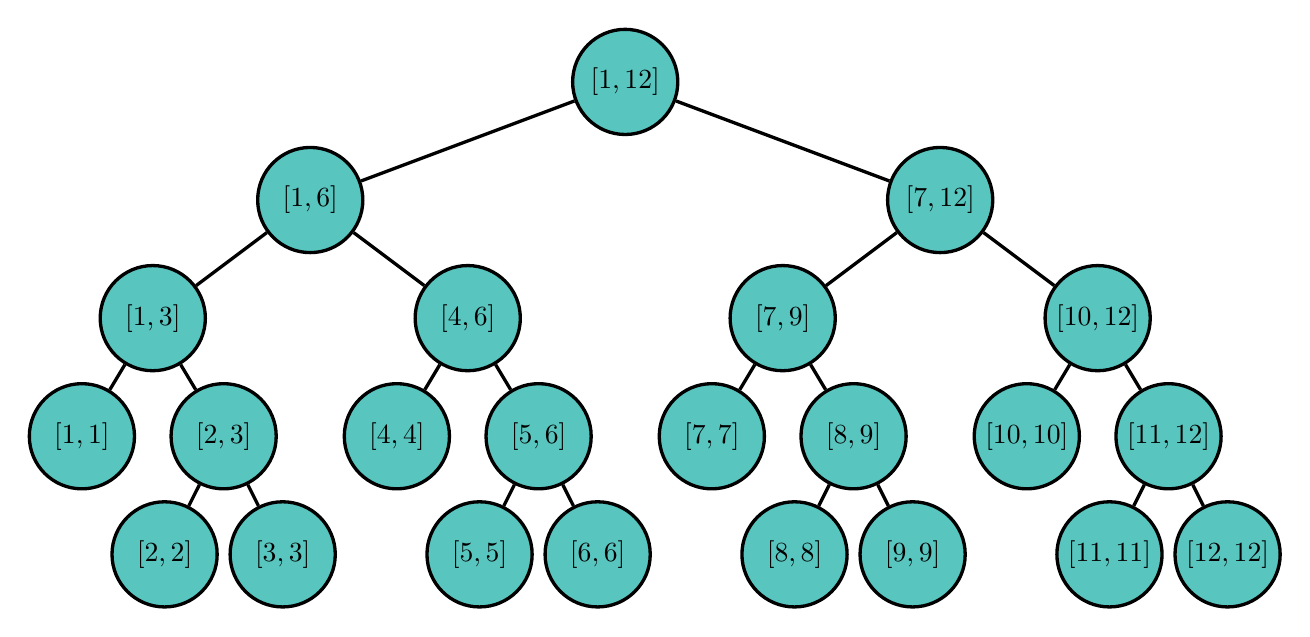
\begin{tikzpicture}[
  very thick,
  level 1/.style={sibling distance=80mm},
  level 2/.style={sibling distance=40mm},
  level 3/.style={sibling distance=18mm},
  level 4/.style={sibling distance=15mm},
]
\node [vertex, minimum size=38pt] (r){$[1,12]$}
  child {
    node [vertex, minimum size=38pt] (a) {$[1,6]$}
    	child {
        	node[vertex, minimum size=38pt] {$[1,3]$}
            	child {
                	node[vertex, minimum size=38pt] {$[1,1]$}
                }
                child {
                	node[vertex, minimum size=38pt] {$[2,3]$}
                    	child {node [vertex, minimum size=38pt] {$[2,2]$}}
                    	child {node [vertex, minimum size=38pt] {$[3,3]$}}
                }
        }
    	child {
        	node[vertex, minimum size=38pt] {$[4,6]$}
            	child {
                	node[vertex, minimum size=38pt] {$[4,4]$}
                }
                child {
                	node[vertex, minimum size=38pt] {$[5,6]$}
                    	child {node [vertex, minimum size=38pt] {$[5,5]$}}
                    	child {node [vertex, minimum size=38pt] {$[6,6]$}}
                }
        }
  }
  child {
    node [vertex, minimum size=38pt] {$[7,12]$}
    	child {
        	node[vertex, minimum size=38pt] {$[7,9]$}
            	child {
                	node[vertex, minimum size=38pt] {$[7,7]$}
                }
                child {
                	node[vertex, minimum size=38pt] {$[8,9]$}
                    	child {node [vertex, minimum size=38pt] {$[8,8]$}}
                    	child {node [vertex, minimum size=38pt] {$[9,9]$}}
                }
        }
    	child {
        	node[vertex, minimum size=38pt] {$[10,12]$}
            	child {
                	node[vertex, minimum size=38pt] {$[10,10]$}
                }
                child {
                	node[vertex, minimum size=38pt] {$[11,12]$}
                    	child {node [vertex, minimum size=38pt] {$[11,11]$}}
                    	child {node [vertex, minimum size=38pt] {$[12,12]$}}
                }
        }
  };

\end{tikzpicture}
}
\end{center}

For this reason, while I used the concept of ``building up'' on top of our array to introduce the segment tree, any operation we implement will start at the root and recursively trickle down the tree. We see that the segment tree structure does not have to resemble a complete tree at all. However, with this approach, it is still quite balanced, so we can store a segment tree within an array as we would a heap.

\subsection{Fenwick Tree}

A \textit{Fenwick tree}, or \textit{binary indexed tree (BIT)}, is simply a faster and easier to code segment tree when the operator in question has an inverse. Unfortunately, it's not at all intuitive, so bear with me at first and let the magic of the Fenwick tree reveal itself later. In fact, it is so magical that Richard Peng hates it. This is a fair sentiment, because it is rather gimmicky. The key idea is to compress the data stored within a segment tree in a crazy way that ends up having a really slick implementation using some bit operation tricks.

As discussed earlier, the $+$ operator has an inverse, $-$. Therefore, there is an inherent redundancy, for example, in keeping track of the sum of the first $\frac{n}{2}$ elements, the sum of all $n$ elements, and the sum of the last $\frac{n}{2}$ elements, as we do in the segment tree. If we are given only $\sum_{k=1}^{n/2} a_k$ and $\sum_{k=1}^n a_k$, we can find $\sum_{k=n/2+1}^{n} a_k$ easily using subtraction.

With this in mind, let's ignore every right child in the tree. We'll mark them as black in the diagram. After that, we'll write out the tree nodes in postfix traversal order, without writing anything whenever we encounter a black node.

\begin{center}
{
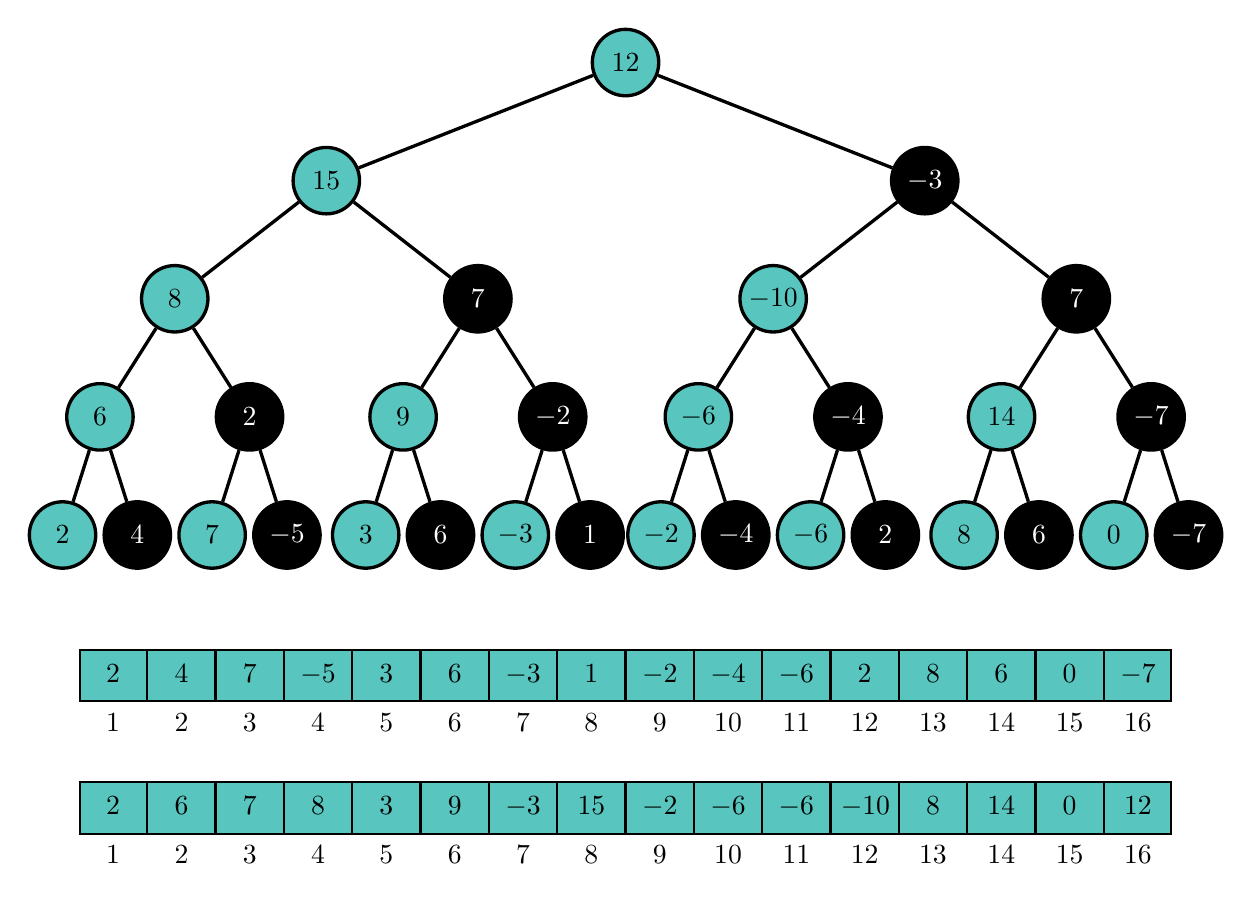
\begin{tikzpicture}[
  very thick,
  level 1/.style={sibling distance=76mm},
  level 2/.style={sibling distance=38.5mm},
  level 3/.style={sibling distance=19mm},
  level 4/.style={sibling distance=9.5mm},
  myrect/.style={
    draw,
    thick,
    fill=myseagreen,
    rectangle split,
    rectangle split horizontal,
    rectangle split parts=#1,
    rectangle split part align=left,
    text width=4ex,
    text centered
    }
]
\node [vertex] (r){$12$}
  child {
    node [vertex] (a) {15}
    child {
      node [vertex] {8}
      child {
        node [vertex] {6}
        child {node [vertex] {2}}
        child {node [vertex, text=mywhite, fill=myblack] {4}}
      } 
      child {
        node [vertex, text=mywhite, fill=myblack] {2}
        child {node [vertex] {7}}
        child {node [vertex, text=mywhite, fill=myblack] {$-5$}}
      }
    }
    child {
      node [vertex, text=mywhite, fill=myblack] {7}
      child {node [vertex] {9}
              child {node [vertex] {3}}
        child {node [vertex, text=mywhite, fill=myblack] {6}}
      }
      child {node [vertex, text=mywhite, fill=myblack] {$-2$}
              child {node [vertex] {$-3$}}
        child {node [vertex, text=mywhite, fill=myblack] {1}}
      }
    }
  }
  child {
    node [vertex, text=mywhite, fill=myblack] {$-3$}
    child {
      node [vertex] {$-10$}
      child {node [vertex] {$-6$}
              child {node [vertex] {$-2$}}
        child {node [vertex, text=mywhite, fill=myblack] {$-4$}}}
      child {node [vertex, text=mywhite, fill=myblack] {$-4$}
              child {node [vertex] {$-6$}}
        child {node [vertex, text=mywhite, fill=myblack] {$2$}}}
    }
    child {
      node [vertex, text=mywhite, fill=myblack] {7}
      child {node [vertex] {14}
              child {node [vertex] {8}}
        child {node [vertex, text=mywhite, fill=myblack] {6}}}
      child {node [vertex, text=mywhite, fill=myblack] {$-7$}
              child {node [vertex] {0}}
        child {node [vertex, text=mywhite, fill=myblack] {$-7$}}}
    }
  };

\node[myrect=16] [below=7cm of r]
  (array)
  {
  					\strut 2
  \nodepart{two}	\strut 4
  \nodepart{three}	\strut 7
  \nodepart{four}	\strut $-5$
  \nodepart{five}	\strut 3
  \nodepart{six}	\strut 6
  \nodepart{seven}	\strut $-3$
  \nodepart{eight}	\strut 1
  \nodepart{nine}	\strut $-2$
  \nodepart{ten}	\strut $-4$
  \nodepart{eleven}	\strut $-6$
  \nodepart{twelve}	\strut 2
  \nodepart{thirteen}	\strut 8
  \nodepart{fourteen}	\strut 6
  \nodepart{fifteen}	\strut 0
  \nodepart{sixteen}	\strut $-7$
  };
\foreach \Valor [count=\Valori from 1] in {one ,two ,three , four , five , six , seven , eight , nine , ten , eleven , twelve , thirteen , fourteen , fifteen , sixteen }
  \node[below] at (array.\Valor south) {\Valori};

\node[myrect=16] [below=of array]
  (array2)
  {
  					\strut 2
  \nodepart{two}	\strut 6
  \nodepart{three}	\strut 7
  \nodepart{four}	\strut 8
  \nodepart{five}	\strut 3
  \nodepart{six}	\strut 9
  \nodepart{seven}	\strut $-3$
  \nodepart{eight}	\strut 15
  \nodepart{nine}	\strut $-2$
  \nodepart{ten}	\strut $-6$
  \nodepart{eleven}	\strut $-6$
  \nodepart{twelve}	\strut $-10$
  \nodepart{thirteen}	\strut 8
  \nodepart{fourteen}	\strut 14
  \nodepart{fifteen}	\strut 0
  \nodepart{sixteen}	\strut 12
  };
\foreach \Valor [count=\Valori from 1] in {one ,two ,three , four , five , six , seven , eight , nine , ten , eleven , twelve , thirteen , fourteen , fifteen , sixteen }
  \node[below] at (array2.\Valor south) {\Valori};

\end{tikzpicture}
}
\end{center}

Our Fenwick tree is simply this last array. This should be quite confusing -- it is not at all clear why this array resembles a tree, and the numbers in the array make no sense whatsoever right now.

Notice that the final position of every unblackened node is just the rightmost black child in its subtree. This leads to the fact that the $i$th element in the Fenwick tree array is the sum

\[b_k = \sum_{k=i-2^{v_2(i)}+1}^i a_k, \]

where $2^{v_2(i)}$ is simply the greatest power of 2 that divides $i$. Let's look at a new diagram that hopefully will better illustrate this key property of the random array we just came up with.

\begin{center}
{
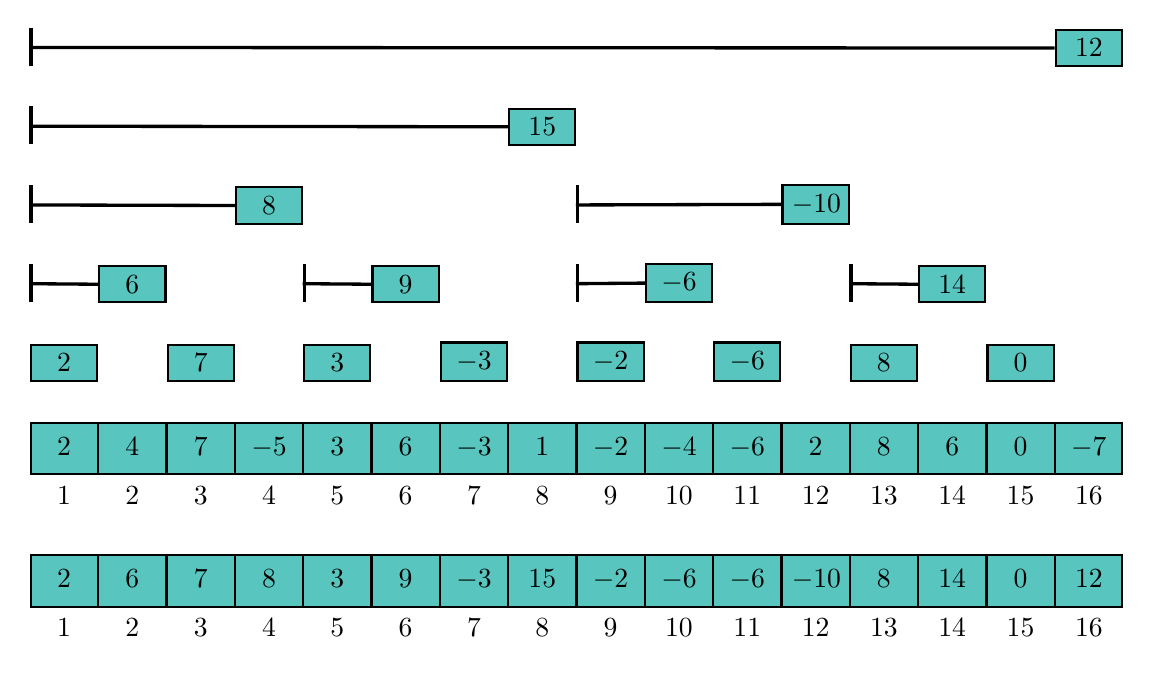
\begin{tikzpicture}[
  very thick,
  myrect/.style={
    draw,
    thick,
    fill=myseagreen,
    rectangle split,
    rectangle split horizontal,
    rectangle split parts=#1,
    rectangle split part align=left,
    text width=4ex,
    text centered
    },
  onesided/.style={
        text width=4ex,
        draw=none,
        append after command={
            [shorten <= -0.5\pgflinewidth] 
            ([shift={( 0.5\pgflinewidth,-0.5\pgflinewidth)}]\tikzlastnode.north west)
        edge([shift={( 0.5\pgflinewidth,+0.5\pgflinewidth)}]\tikzlastnode.south west)            
        }
    }
]

\node[myrect=16]
  (array)
  {
  					\strut 2
  \nodepart{two}	\strut 4
  \nodepart{three}	\strut 7
  \nodepart{four}	\strut $-5$
  \nodepart{five}	\strut 3
  \nodepart{six}	\strut 6
  \nodepart{seven}	\strut $-3$
  \nodepart{eight}	\strut 1
  \nodepart{nine}	\strut $-2$
  \nodepart{ten}	\strut $-4$
  \nodepart{eleven}	\strut $-6$
  \nodepart{twelve}	\strut 2
  \nodepart{thirteen}	\strut 8
  \nodepart{fourteen}	\strut 6
  \nodepart{fifteen}	\strut 0
  \nodepart{sixteen}	\strut $-7$
  };
\foreach \Valor [count=\Valori from 1] in {one ,two ,three , four , five , six , seven , eight , nine , ten , eleven , twelve , thirteen , fourteen , fifteen , sixteen }
  \node[below] at (array.\Valor south) {\Valori};

\node[myrect=1, above=5mm] at (array.one north) (n1) {2};
\node[myrect=1, above=15mm] at (array.two north) (n2) {6};
\node[myrect=1, above=5mm] at (array.three north) (n3) {7};
\node[myrect=1, above=25mm] at (array.four north) (n4) {8};
\node[myrect=1, above=5mm] at (array.five north) (n5) {3};
\node[myrect=1, above=15mm] at (array.six north) (n6) {9};
\node[myrect=1, above=5mm] at (array.seven north) (n7) {$-3$};
\node[myrect=1, above=35mm] at (array.eight north) (n8) {15};
\node[myrect=1, above=5mm] at (array.nine north) (n9) {$-2$};
\node[myrect=1, above=15mm] at (array.ten north) (n10) {$-6$};
\node[myrect=1, above=5mm] at (array.eleven north) (n11) {$-6$};
\node[myrect=1, above=25mm] at (array.twelve north) (n12) {$-10$};
\node[myrect=1, above=5mm] at (array.thirteen north) (n13) {8};
\node[myrect=1, above=15mm] at (array.fourteen north) (n14) {14};
\node[myrect=1, above=5mm] at (array.fifteen north) (n15) {0};
\node[myrect=1, above=45mm] at (array.sixteen north) (n16) {12};

\node[onesided, above=15mm] at (array.one north) (m2) { \phantom{0} };
\node[onesided, above=25mm] at (array.one north) (m4) { \phantom{0} };
\node[onesided, above=15mm] at (array.five north) (m6) { \phantom{0} };
\node[onesided, above=35mm] at (array.one north) (m8) { \phantom{0} };
\node[onesided, above=15mm] at (array.nine north) (m10) { \phantom{0} };
\node[onesided, above=25mm] at (array.nine north) (m12) { \phantom{0} };
\node[onesided, above=15mm] at (array.thirteen north) (m14) { \phantom{0} };
\node[onesided, above=45mm] at (array.one north) (m16) { \phantom{0} };

\draw (m2.west) -- (n2.west);
\draw (m4.west) -- (n4.west);
\draw (m6.west) -- (n6.west);
\draw (m8.west) -- (n8.west);
\draw (m10.west) -- (n10.west);
\draw (m12.west) -- (n12.west);
\draw (m14.west) -- (n14.west);
\draw (m16.west) -- (n16.west);

\node[myrect=16] [below=of array]
  (array2)
  {
  					\strut 2
  \nodepart{two}	\strut 6
  \nodepart{three}	\strut 7
  \nodepart{four}	\strut 8
  \nodepart{five}	\strut 3
  \nodepart{six}	\strut 9
  \nodepart{seven}	\strut $-3$
  \nodepart{eight}	\strut 15
  \nodepart{nine}	\strut $-2$
  \nodepart{ten}	\strut $-6$
  \nodepart{eleven}	\strut $-6$
  \nodepart{twelve}	\strut $-10$
  \nodepart{thirteen}	\strut 8
  \nodepart{fourteen}	\strut 14
  \nodepart{fifteen}	\strut 0
  \nodepart{sixteen}	\strut 12
  };
\foreach \Valor [count=\Valori from 1] in {one ,two ,three , four , five , six , seven , eight , nine , ten , eleven , twelve , thirteen , fourteen , fifteen , sixteen }
  \node[below] at (array2.\Valor south) {\Valori};

\end{tikzpicture}
}
\end{center}

All the framework is now in place. Now we need to find out how to query and update the Fenwick tree.

Suppose we wanted to find the sum $\sum_{k=1}^{11} a_k$. Let's take a look at the diagram to see which elements we need.

\begin{center}
{
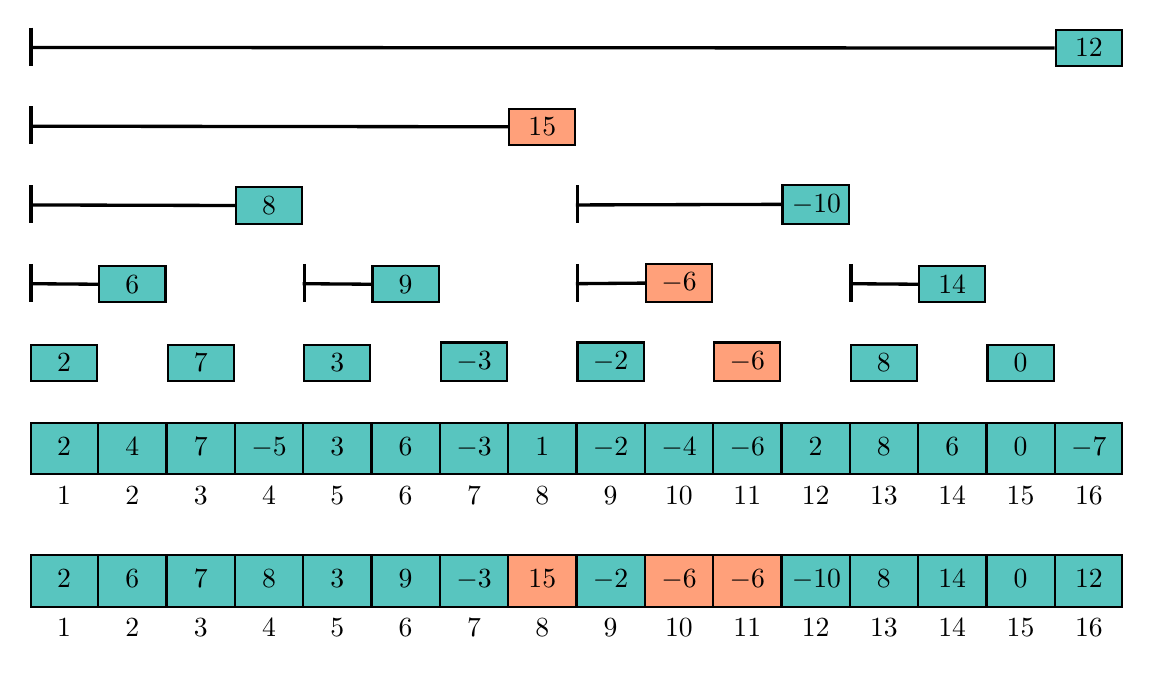
\begin{tikzpicture}[
  very thick,
  myrect2/.style={
    draw,
    thick,
    rectangle split,
    rectangle split horizontal,
    rectangle split parts=#1,
    rectangle split part align=left,
    text width=4ex,
    text centered
    },
  myrect/.style={
    draw,
    thick,
    rectangle split,
    rectangle split horizontal,
    rectangle split parts=#1,
    fill=myseagreen,
    rectangle split part align=left,
    text width=4ex,
    text centered,
  	fill=myseagreen
  },
  onesided/.style={
        text width=4ex,
        draw=none,
        append after command={
            [shorten <= -0.5\pgflinewidth] 
            ([shift={( 0.5\pgflinewidth,-0.5\pgflinewidth)}]\tikzlastnode.north west)
        edge([shift={( 0.5\pgflinewidth,+0.5\pgflinewidth)}]\tikzlastnode.south west)            
        }
    }
]

\node[myrect=16]
  (array)
  {
  					\strut 2
  \nodepart{two}	\strut 4
  \nodepart{three}	\strut 7
  \nodepart{four}	\strut $-5$
  \nodepart{five}	\strut 3
  \nodepart{six}	\strut 6
  \nodepart{seven}	\strut $-3$
  \nodepart{eight}	\strut 1
  \nodepart{nine}	\strut $-2$
  \nodepart{ten}	\strut $-4$
  \nodepart{eleven}	\strut $-6$
  \nodepart{twelve}	\strut 2
  \nodepart{thirteen}	\strut 8
  \nodepart{fourteen}	\strut 6
  \nodepart{fifteen}	\strut 0
  \nodepart{sixteen}	\strut $-7$
  };
\foreach \Valor [count=\Valori from 1] in {one ,two ,three , four , five , six , seven , eight , nine , ten , eleven , twelve , thirteen , fourteen , fifteen , sixteen }
  \node[below] at (array.\Valor south) {\Valori};

\node[myrect=1, above=5mm] at (array.one north) (n1) {2};
\node[myrect=1, above=15mm] at (array.two north) (n2) {6};
\node[myrect=1, above=5mm] at (array.three north) (n3) {7};
\node[myrect=1, above=25mm] at (array.four north) (n4) {8};
\node[myrect=1, above=5mm] at (array.five north) (n5) {3};
\node[myrect=1, above=15mm] at (array.six north) (n6) {9};
\node[myrect=1, above=5mm] at (array.seven north) (n7) {$-3$};
\node[myrect=1, above=35mm, fill=mysalmon] at (array.eight north) (n8) {15};
\node[myrect=1, above=5mm] at (array.nine north) (n9) {$-2$};
\node[myrect=1, above=15mm, fill=mysalmon] at (array.ten north) (n10) {$-6$};
\node[myrect=1, above=5mm, fill=mysalmon] at (array.eleven north) (n11) {$-6$};
\node[myrect=1, above=25mm] at (array.twelve north) (n12) {$-10$};
\node[myrect=1, above=5mm] at (array.thirteen north) (n13) {8};
\node[myrect=1, above=15mm] at (array.fourteen north) (n14) {14};
\node[myrect=1, above=5mm] at (array.fifteen north) (n15) {0};
\node[myrect=1, above=45mm] at (array.sixteen north) (n16) {12};

\node[onesided, above=15mm] at (array.one north) (m2) { \phantom{0} };
\node[onesided, above=25mm] at (array.one north) (m4) { \phantom{0} };
\node[onesided, above=15mm] at (array.five north) (m6) { \phantom{0} };
\node[onesided, above=35mm] at (array.one north) (m8) { \phantom{0} };
\node[onesided, above=15mm] at (array.nine north) (m10) { \phantom{0} };
\node[onesided, above=25mm] at (array.nine north) (m12) { \phantom{0} };
\node[onesided, above=15mm] at (array.thirteen north) (m14) { \phantom{0} };
\node[onesided, above=45mm] at (array.one north) (m16) { \phantom{0} };

\draw (m2.west) -- (n2.west);
\draw (m4.west) -- (n4.west);
\draw (m6.west) -- (n6.west);
\draw (m8.west) -- (n8.west);
\draw (m10.west) -- (n10.west);
\draw (m12.west) -- (n12.west);
\draw (m14.west) -- (n14.west);
\draw (m16.west) -- (n16.west);

\node[myrect2=16, rectangle split part fill={myseagreen, myseagreen, myseagreen, myseagreen, myseagreen, myseagreen, myseagreen, mysalmon, myseagreen, mysalmon, mysalmon, myseagreen, myseagreen, myseagreen, myseagreen, myseagreen}] [below=of array]
  (array2)
  {
  					\strut 2
  \nodepart{two}	\strut 6
  \nodepart{three}	\strut 7
  \nodepart{four}	\strut 8
  \nodepart{five}	\strut 3
  \nodepart{six}	\strut 9
  \nodepart{seven}	\strut $-3$
  \nodepart{eight}	\strut 15
  \nodepart{nine}	\strut $-2$
  \nodepart{ten}	\strut $-6$
  \nodepart{eleven}	\strut $-6$
  \nodepart{twelve}	\strut $-10$
  \nodepart{thirteen}	\strut 8
  \nodepart{fourteen}	\strut 14
  \nodepart{fifteen}	\strut 0
  \nodepart{sixteen}	\strut 12
  };
\foreach \Valor [count=\Valori from 1] in {one ,two ,three , four , five , six , seven , eight , nine , ten , eleven , twelve , thirteen , fourteen , fifteen , sixteen }
  \node[below] at (array2.\Valor south) {\Valori};

\end{tikzpicture}
}
\end{center}

We see that the sum $\sum_{k=1}^{11}a_k=b_8+b_{10}+b_{11}$. If we look at 11 in binary, we have $11=01011_2$. Let's see if we can find a pattern in these numbers in binary:

\begin{align*}
11 &= 01011_2, \\
10 = 11-2^{v_2(11)} &= 01010_2, \\
8 = 10-2^{v_2(10)} &= 01000_2, \\
0=8-2^{v_2(8)}&=00000_2.
\end{align*}

So, we can simply subtract $11-2^{v_2(11)}=10=01010_2$, find the sum of the first 10 elements, and add $b_{11}$ to that sum to get the sum of the first 11 elements. We see that repeating this process takes off the last 1 in the binary representation of the number $i$, and since there are at most $\log{n}+1$ 1s in the binary representation $\forall i \in [1,n]$, the query operation is $O(\log{n})$.

And now for the update operation. Suppose we want to change the value of $a_{11}$ from $-6$ to $-3$. Which numbers will we have to change?

\begin{center}
{
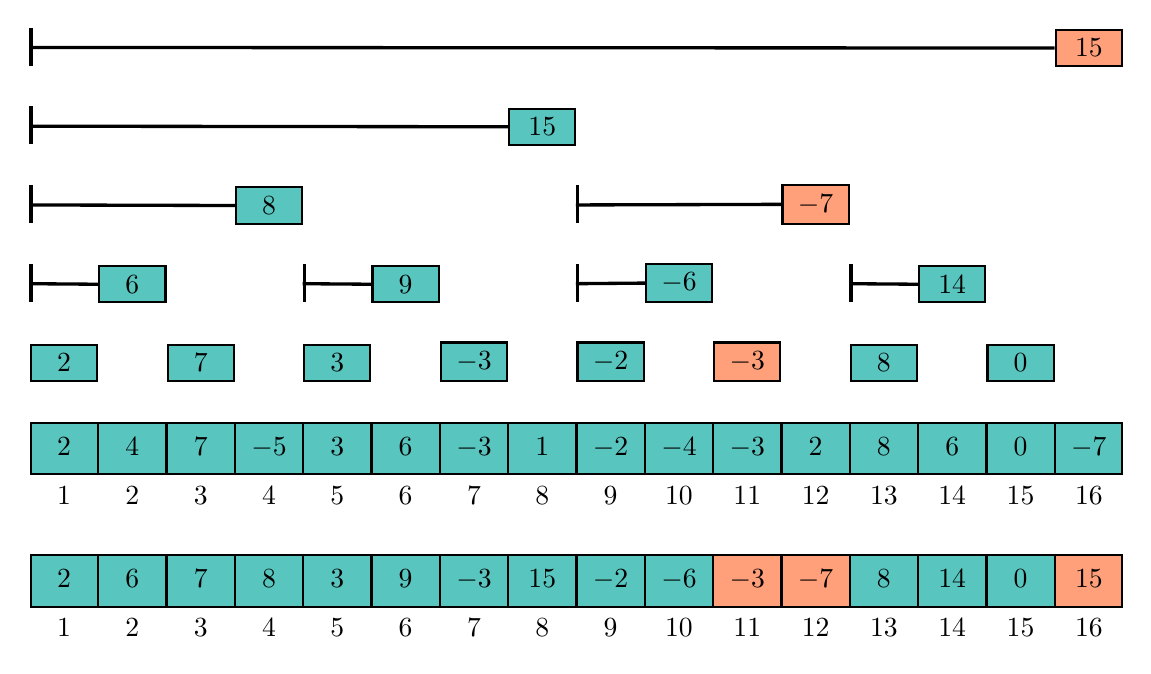
\begin{tikzpicture}[
  very thick,
  myrect2/.style={
    draw,
    thick,
    rectangle split,
    rectangle split horizontal,
    rectangle split parts=#1,
    rectangle split part align=left,
    text width=4ex,
    text centered
    },
  myrect/.style={
    draw,
    thick,
    rectangle split,
    rectangle split horizontal,
    rectangle split parts=#1,
    fill=myseagreen,
    rectangle split part align=left,
    text width=4ex,
    text centered,
  	fill=myseagreen
  },
  onesided/.style={
        text width=4ex,
        draw=none,
        append after command={
            [shorten <= -0.5\pgflinewidth] 
            ([shift={( 0.5\pgflinewidth,-0.5\pgflinewidth)}]\tikzlastnode.north west)
        edge([shift={( 0.5\pgflinewidth,+0.5\pgflinewidth)}]\tikzlastnode.south west)            
        }
    }
]

\node[myrect=16]
  (array)
  {
  					\strut 2
  \nodepart{two}	\strut 4
  \nodepart{three}	\strut 7
  \nodepart{four}	\strut $-5$
  \nodepart{five}	\strut 3
  \nodepart{six}	\strut 6
  \nodepart{seven}	\strut $-3$
  \nodepart{eight}	\strut 1
  \nodepart{nine}	\strut $-2$
  \nodepart{ten}	\strut $-4$
  \nodepart{eleven}	\strut $-3$
  \nodepart{twelve}	\strut 2
  \nodepart{thirteen}	\strut 8
  \nodepart{fourteen}	\strut 6
  \nodepart{fifteen}	\strut 0
  \nodepart{sixteen}	\strut $-7$
  };
\foreach \Valor [count=\Valori from 1] in {one ,two ,three , four , five , six , seven , eight , nine , ten , eleven , twelve , thirteen , fourteen , fifteen , sixteen }
  \node[below] at (array.\Valor south) {\Valori};

\node[myrect=1, above=5mm] at (array.one north) (n1) {2};
\node[myrect=1, above=15mm] at (array.two north) (n2) {6};
\node[myrect=1, above=5mm] at (array.three north) (n3) {7};
\node[myrect=1, above=25mm] at (array.four north) (n4) {8};
\node[myrect=1, above=5mm] at (array.five north) (n5) {3};
\node[myrect=1, above=15mm] at (array.six north) (n6) {9};
\node[myrect=1, above=5mm] at (array.seven north) (n7) {$-3$};
\node[myrect=1, above=35mm] at (array.eight north) (n8) {15};
\node[myrect=1, above=5mm] at (array.nine north) (n9) {$-2$};
\node[myrect=1, above=15mm] at (array.ten north) (n10) {$-6$};
\node[myrect=1, above=5mm, fill=mysalmon] at (array.eleven north) (n11) {$-3$};
\node[myrect=1, above=25mm, fill=mysalmon] at (array.twelve north) (n12) {$-7$};
\node[myrect=1, above=5mm] at (array.thirteen north) (n13) {8};
\node[myrect=1, above=15mm] at (array.fourteen north) (n14) {14};
\node[myrect=1, above=5mm] at (array.fifteen north) (n15) {0};
\node[myrect=1, above=45mm, fill=mysalmon] at (array.sixteen north) (n16) {15};

\node[onesided, above=15mm] at (array.one north) (m2) { \phantom{0} };
\node[onesided, above=25mm] at (array.one north) (m4) { \phantom{0} };
\node[onesided, above=15mm] at (array.five north) (m6) { \phantom{0} };
\node[onesided, above=35mm] at (array.one north) (m8) { \phantom{0} };
\node[onesided, above=15mm] at (array.nine north) (m10) { \phantom{0} };
\node[onesided, above=25mm] at (array.nine north) (m12) { \phantom{0} };
\node[onesided, above=15mm] at (array.thirteen north) (m14) { \phantom{0} };
\node[onesided, above=45mm] at (array.one north) (m16) { \phantom{0} };

\draw (m2.west) -- (n2.west);
\draw (m4.west) -- (n4.west);
\draw (m6.west) -- (n6.west);
\draw (m8.west) -- (n8.west);
\draw (m10.west) -- (n10.west);
\draw (m12.west) -- (n12.west);
\draw (m14.west) -- (n14.west);
\draw (m16.west) -- (n16.west);

\node[myrect2=16, rectangle split part fill={myseagreen, myseagreen, myseagreen, myseagreen, myseagreen, myseagreen, myseagreen, myseagreen, myseagreen, myseagreen, mysalmon, mysalmon, myseagreen, myseagreen, myseagreen, mysalmon}] [below=of array]
  (array2)
  {
  					\strut 2
  \nodepart{two}	\strut 6
  \nodepart{three}	\strut 7
  \nodepart{four}	\strut 8
  \nodepart{five}	\strut 3
  \nodepart{six}	\strut 9
  \nodepart{seven}	\strut $-3$
  \nodepart{eight}	\strut 15
  \nodepart{nine}	\strut $-2$
  \nodepart{ten}	\strut $-6$
  \nodepart{eleven}	\strut $-3$
  \nodepart{twelve}	\strut $-7$
  \nodepart{thirteen}	\strut 8
  \nodepart{fourteen}	\strut 14
  \nodepart{fifteen}	\strut 0
  \nodepart{sixteen}	\strut 15
  };
\foreach \Valor [count=\Valori from 1] in {one ,two ,three , four , five , six , seven , eight , nine , ten , eleven , twelve , thirteen , fourteen , fifteen , sixteen }
  \node[below] at (array2.\Valor south) {\Valori};

\end{tikzpicture}
}
\end{center}

We needed to increment the highlighted values, $b_{11}$, $b_{12}$, and $b_{16}$, by 3. Once again we'll look at 11, 12, and 16 in base 2.

\begin{align*}
11 &= 01011_2, \\
12 &= 01100_2 = 11 + 2^{v_2(11)}, \\
16 &= 10000_2 = 12 + 2^{v_2(12)}.
\end{align*}

It appears that instead of subtracting the largest dividing power of 2, we are adding. Once again this is an $O(\log{n})$ operation.

The real magic in the Fenwick tree is how quickly it can be coded. The only tricky part is finding exactly what $2^{v_2(i)}$ is. But it turns out, by the way bits are arranged in negative numbers, this is just \texttt{i \& -i}. With this in mind, here's all the code that's necessary to code a Fenwick tree.

\begin{mylstlisting}
int[] b = new int[MAXN]; // Fenwick tree stored as array
void update(int i, int x) {
	for( ; i < MAXN; i += i & -i)
		b[i] += x;
}
int prefixSum(int i) {
	int sum = 0;
	for( ; i > 0; i -= i & -i)
		sum += b[i];
	return sum;
}
int query(int i, int j) {
	return prefixSum(j) - prefixSum(i - 1);
}
\end{mylstlisting}

\subsection{Lazy Propagation}

It is often the case that in addition to performing range queries, we need to be able to perform \textit{range updates}. (Before, we only had to implement point updates.) One extension of our sum problem would require the following two functions:

\begin{itemize}
\item
$update(i, j, x)$ -- increment the value of $a_k$ by $x$ for all $k\in [i,j]$

\item
$query(i, j)$ -- return $\sum_{k=i}^j a_k$.
\end{itemize}

\subsubsection{Some Motivation: $\sqrt{n}$ Blocking}

Let's go back to our $\sqrt{n}$ blocking solution and see what changes we can make, and hopefully we can extend this idea back to our segment tree. If we're looking for an $O(\sqrt{n})$ implementation for $update$, we clearly can't perform point updates for all values in the range. The way we sped up $query$ was by keeping track of an extra set of data, the sum of all the elements in a bucket, which we used when \textit{the entire bucket was in the query range}.

\begin{center}
{
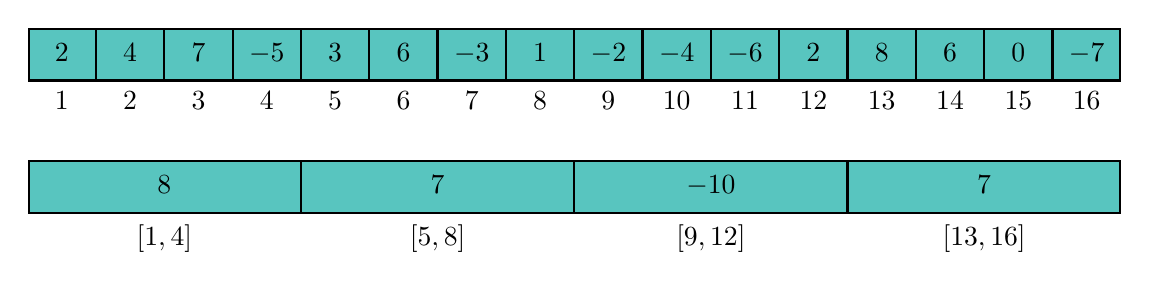
\begin{tikzpicture}[
  thick,
  myrect/.style={
    draw,
    fill=myseagreen,
    rectangle split,
    rectangle split horizontal,
    rectangle split parts=#1,
    rectangle split part align=left,
    text width=4ex,
    text centered
    }
]

\node[myrect=16]
  (array2)
  {
  					\strut 2
  \nodepart{two}	\strut 4
  \nodepart{three}	\strut 7
  \nodepart{four}	\strut $-5$
  \nodepart{five}	\strut 3
  \nodepart{six}	\strut 6
  \nodepart{seven}	\strut $-3$
  \nodepart{eight}	\strut 1
  \nodepart{nine}	\strut $-2$
  \nodepart{ten}	\strut $-4$
  \nodepart{eleven}	\strut $-6$
  \nodepart{twelve}	\strut 2
  \nodepart{thirteen}	\strut 8
  \nodepart{fourteen}	\strut 6
  \nodepart{fifteen}	\strut 0
  \nodepart{sixteen}	\strut $-7$
  };
\foreach \Valor [count=\Valori from 1] in {one ,two ,three , four , five , six , seven , eight , nine , ten , eleven , twelve , thirteen , fourteen , fifteen , sixteen }
  \node[below] at (array2.\Valor south) {\Valori};

\node[myrect=4, text width=21.2ex] [below=of array2]
  (array)
  {
  					\strut 8
  \nodepart{two}	\strut 7
  \nodepart{three}	\strut $-10$
  \nodepart{four}	\strut 7
  };

\node[below] at (array.one south) {$[1,4]$};
\node[below] at (array.two south) {$[5,8]$};
\node[below] at (array.three south) {$[9,12]$};
\node[below] at (array.four south) {$[13,16]$};
\end{tikzpicture}
}
\end{center}

What can we do with this idea for $update$? Let's see what we can do if an entire bucket were included in the update range. Again, we don't want to touch the original array $a$ at all since that makes the operation linear. Let's try storing some information separately. This other information we're storing is the key idea behind lazy propagation.

With this in mind, highlighted are the elements we'll need for $update(4,14,3)$.

\begin{center}
{
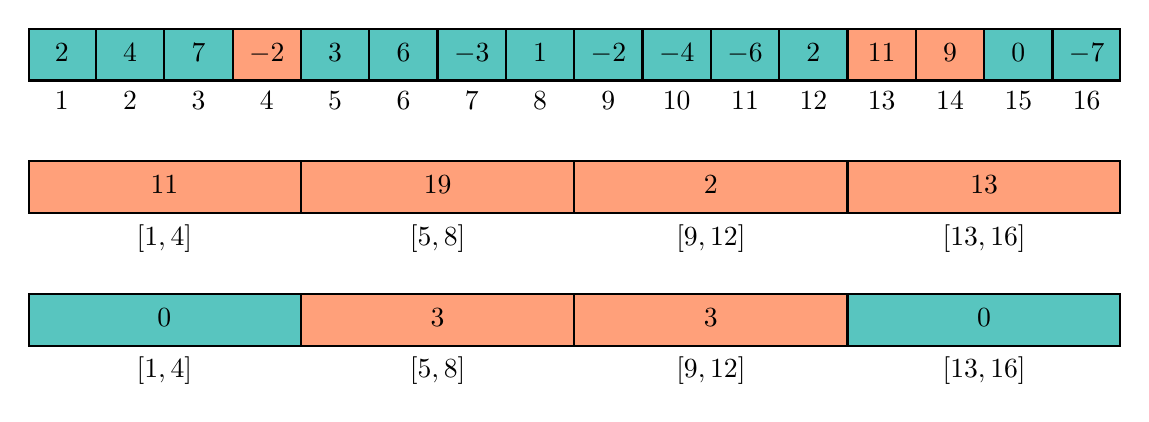
\begin{tikzpicture}[
  thick,
  myrect/.style={
    draw,
    rectangle split,
    rectangle split horizontal,
    rectangle split parts=#1,
    rectangle split part align=left,
    text width=4ex,
    text centered
    }
]

\node[myrect=16, rectangle split part fill={myseagreen, myseagreen, myseagreen, mysalmon, myseagreen, myseagreen, myseagreen, myseagreen, myseagreen, myseagreen, myseagreen, myseagreen, mysalmon, mysalmon, myseagreen, myseagreen}]
  (array2)
  {
  					\strut 2
  \nodepart{two}	\strut 4
  \nodepart{three}	\strut 7
  \nodepart{four}	\strut $-2$
  \nodepart{five}	\strut 3
  \nodepart{six}	\strut 6
  \nodepart{seven}	\strut $-3$
  \nodepart{eight}	\strut 1
  \nodepart{nine}	\strut $-2$
  \nodepart{ten}	\strut $-4$
  \nodepart{eleven}	\strut $-6$
  \nodepart{twelve}	\strut 2
  \nodepart{thirteen}	\strut 11
  \nodepart{fourteen}	\strut 9
  \nodepart{fifteen}	\strut 0
  \nodepart{sixteen}	\strut $-7$
  };
\foreach \Valor [count=\Valori from 1] in {one ,two ,three , four , five , six , seven , eight , nine , ten , eleven , twelve , thirteen , fourteen , fifteen , sixteen }
  \node[below] at (array2.\Valor south) {\Valori};

\node[myrect=4, text width=21.2ex, rectangle split part fill={mysalmon, mysalmon, mysalmon, mysalmon}] [below=of array2]
  (array)
  {
  					\strut 11
  \nodepart{two}	\strut 19
  \nodepart{three}	\strut 2
  \nodepart{four}	\strut 13
  };

\node[below] at (array.one south) {$[1,4]$};
\node[below] at (array.two south) {$[5,8]$};
\node[below] at (array.three south) {$[9,12]$};
\node[below] at (array.four south) {$[13,16]$};

\node[myrect=4, text width=21.2ex, rectangle split part fill={myseagreen, mysalmon, mysalmon, myseagreen}] [below=of array]
  (array3)
  {
  					\strut 0
  \nodepart{two}	\strut 3
  \nodepart{three}	\strut 3
  \nodepart{four}	\strut 0
  };

\node[below] at (array3.one south) {$[1,4]$};
\node[below] at (array3.two south) {$[5,8]$};
\node[below] at (array3.three south) {$[9,12]$};
\node[below] at (array3.four south) {$[13,16]$};
\end{tikzpicture}
}
\end{center}

Note that the sums associated with each bucket must adjust appropriately. In the example, there are four elements per bucket, so when an entire bucket needs to be incremented by 3, a single bucket can increment its sum by $4 \cdot 3 = 12$ easily.

To reiterate, we not storing the actual values of the elements where they were stored in solving the original formulation of the problem. Despite this fact, we are able to calculate what any single value is supposed to be. $a_i$ is simply equal to the $\ceiling{\frac{i}{\sqrt{n}}}$th value stored in the newest third array added to the $i$th value stored in the first array. Because of this, querying a range works in almost exactly the same way as it did in the original formulation.

Highlighted are the values necessary for $query(7,15)$.

\begin{center}
{
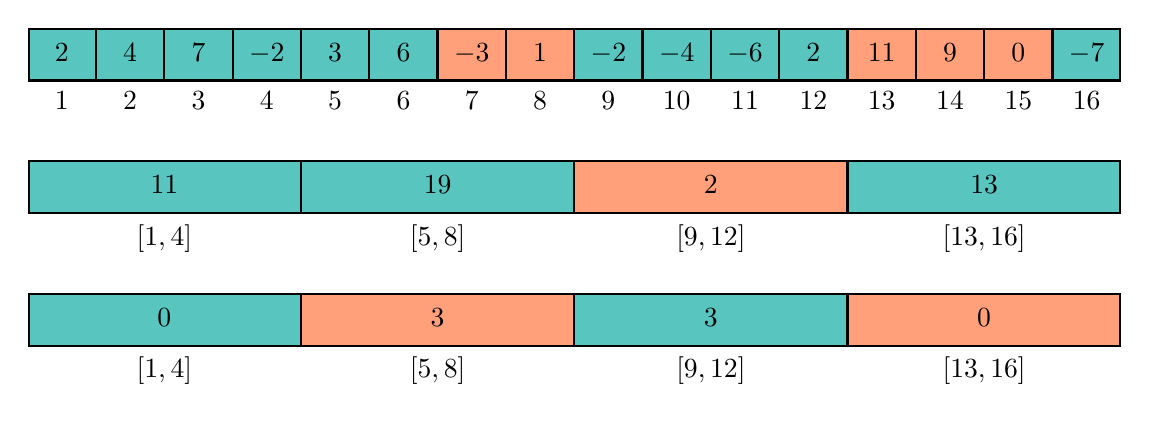
\begin{tikzpicture}[
  thick,
  myrect/.style={
    draw,
    rectangle split,
    rectangle split horizontal,
    rectangle split parts=#1,
    rectangle split part align=left,
    text width=4ex,
    text centered
    }
]

\node[myrect=16, rectangle split part fill={myseagreen, myseagreen, myseagreen, myseagreen, myseagreen, myseagreen, mysalmon, mysalmon, myseagreen, myseagreen, myseagreen, myseagreen, mysalmon, mysalmon, mysalmon, myseagreen}]
  (array2)
  {
  					\strut 2
  \nodepart{two}	\strut 4
  \nodepart{three}	\strut 7
  \nodepart{four}	\strut $-2$
  \nodepart{five}	\strut 3
  \nodepart{six}	\strut 6
  \nodepart{seven}	\strut $-3$
  \nodepart{eight}	\strut 1
  \nodepart{nine}	\strut $-2$
  \nodepart{ten}	\strut $-4$
  \nodepart{eleven}	\strut $-6$
  \nodepart{twelve}	\strut 2
  \nodepart{thirteen}	\strut 11
  \nodepart{fourteen}	\strut 9
  \nodepart{fifteen}	\strut 0
  \nodepart{sixteen}	\strut $-7$
  };
\foreach \Valor [count=\Valori from 1] in {one ,two ,three , four , five , six , seven , eight , nine , ten , eleven , twelve , thirteen , fourteen , fifteen , sixteen }
  \node[below] at (array2.\Valor south) {\Valori};

\node[myrect=4, text width=21.2ex, rectangle split part fill={myseagreen, myseagreen, mysalmon, myseagreen}] [below=of array2]
  (array)
  {
  					\strut 11
  \nodepart{two}	\strut 19
  \nodepart{three}	\strut 2
  \nodepart{four}	\strut 13
  };

\node[below] at (array.one south) {$[1,4]$};
\node[below] at (array.two south) {$[5,8]$};
\node[below] at (array.three south) {$[9,12]$};
\node[below] at (array.four south) {$[13,16]$};

\node[myrect=4, text width=21.2ex, rectangle split part fill={myseagreen, mysalmon, myseagreen, mysalmon}] [below=of array]
  (array3)
  {
  					\strut 0
  \nodepart{two}	\strut 3
  \nodepart{three}	\strut 3
  \nodepart{four}	\strut 0
  };

\node[below] at (array3.one south) {$[1,4]$};
\node[below] at (array3.two south) {$[5,8]$};
\node[below] at (array3.three south) {$[9,12]$};
\node[below] at (array3.four south) {$[13,16]$};
\end{tikzpicture}
}
\end{center}

Thus we have achieved $O(\sqrt{n})$ for both range updates and and range queries.

\subsubsection{Lazy Propagation on a Segment Tree}

Motivated by how we fixed our $O(\sqrt{n})$ solution, let's try adding a similar extra piece of information to our segment tree to try to get an $O(\log{n})$ solution. Let's call this extra number the ``lazy'' number.

\begin{center}
{
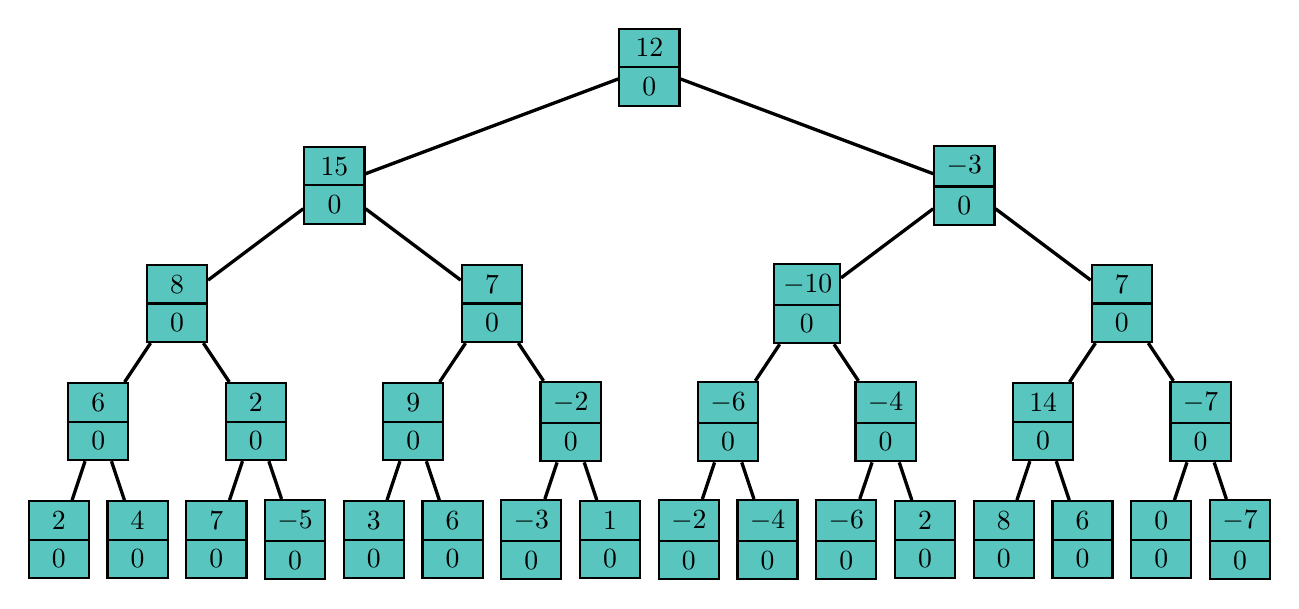
\begin{tikzpicture}[
  very thick,
  level 1/.style={sibling distance=80mm},
  level 2/.style={sibling distance=40mm},
  level 3/.style={sibling distance=20mm},
  level 4/.style={sibling distance=10mm},
  myrect/.style={
    draw,
    thick,
    fill=myseagreen,
    rectangle split,
    rectangle split parts=2,
    rectangle split part align=left,
    text width=3.5ex,
    text centered
    }
]
\node [myrect] (r){$12$\nodepart{two}0}
  child {
    node [myrect] (a) {15\nodepart{two}0}
    child {
      node [myrect] {8\nodepart{two}0}
      child {
        node [myrect] {6\nodepart{two}0}
        child {node [myrect] {2\nodepart{two}0}}
        child {node [myrect] {4\nodepart{two}0}}
      } 
      child {
        node [myrect] {2\nodepart{two}0}
        child {node [myrect] {7\nodepart{two}0}}
        child {node [myrect] {$-5$\nodepart{two}0}}
      }
    }
    child {
      node [myrect] {7\nodepart{two}0}
      child {node [myrect] {9\nodepart{two}0}
              child {node [myrect] {3\nodepart{two}0}}
        child {node [myrect] {6\nodepart{two}0}}
      }
      child {node [myrect] {$-2$\nodepart{two}0}
              child {node [myrect] {$-3$\nodepart{two}0}}
        child {node [myrect] {1\nodepart{two}0}}
      }
    }
  }
  child {
    node [myrect] {$-3$\nodepart{two}0}
    child {
      node [myrect, text width=4ex] {$-10$\nodepart{two}0}
      child {node [myrect] {$-6$\nodepart{two}0}
              child {node [myrect] {$-2$\nodepart{two}0}}
        child {node [myrect] {$-4$\nodepart{two}0}}}
      child {node [myrect] {$-4$\nodepart{two}0}
              child {node [myrect] {$-6$\nodepart{two}0}}
        child {node [myrect] {$2$\nodepart{two}0}}}
    }
    child {
      node [myrect] {7\nodepart{two}0}
      child {node [myrect] {14\nodepart{two}0}
              child {node [myrect] {8\nodepart{two}0}}
        child {node [myrect] {6\nodepart{two}0}}}
      child {node [myrect] {$-7$\nodepart{two}0}
              child {node [myrect] {0\nodepart{two}0}}
        child {node [myrect] {$-7$\nodepart{two}0}}}
    }
  };

\end{tikzpicture}
}
\end{center}

Once again, if the entire range associated with a node is contained within the update interval, we'll just make a note of it on that particular node and not update any of its children. We'll call such a node ``lazy.''

Here's the status of the tree after $update(3,12,2)$.

\begin{center}
{
\begin{tikzpicture}[
  very thick,
  level 1/.style={sibling distance=80mm},
  level 2/.style={sibling distance=40mm},
  level 3/.style={sibling distance=20mm},
  level 4/.style={sibling distance=10mm},
  myrect/.style={
    draw,
    thick,
    rectangle split,
    rectangle split parts=2,
    rectangle split part fill={myseagreen, myseagreen},
    rectangle split part align=left,
    text width=3.5ex,
    text centered
    }
]
\node [myrect, rectangle split part fill={mysalmon, myseagreen}] (r){$32$\nodepart{two}0}
  child {
    node [myrect, rectangle split part fill={mysalmon, myseagreen}] (a) {27\nodepart{two}0}
    child {
      node [myrect, rectangle split part fill={mysalmon, myseagreen}] {12\nodepart{two}0}
      child {
        node [myrect] {6\nodepart{two}0}
        child {node [myrect] {2\nodepart{two}0}}
        child {node [myrect] {4\nodepart{two}0}}
      } 
      child {
        node [myrect, rectangle split part fill={mysalmon, mysalmon}] {6\nodepart{two}2}
        child {node [myrect] {7\nodepart{two}0}}
        child {node [myrect] {$-5$\nodepart{two}0}}
      }
    }
    child {
      node [myrect, rectangle split part fill={mysalmon, mysalmon}] {15\nodepart{two}2}
      child {node [myrect] {9\nodepart{two}0}
              child {node [myrect] {3\nodepart{two}0}}
        child {node [myrect] {6\nodepart{two}0}}
      }
      child {node [myrect] {$-2$\nodepart{two}0}
              child {node [myrect] {$-3$\nodepart{two}0}}
        child {node [myrect] {1\nodepart{two}0}}
      }
    }
  }
  child {
    node [myrect, rectangle split part fill={mysalmon, myseagreen}] {$5$\nodepart{two}0}
    child {
      node [myrect, rectangle split part fill={mysalmon, mysalmon}] {$-2$\nodepart{two}2}
      child {node [myrect] {$-6$\nodepart{two}0}
              child {node [myrect] {$-2$\nodepart{two}0}}
        child {node [myrect] {$-4$\nodepart{two}0}}}
      child {node [myrect] {$-4$\nodepart{two}0}
              child {node [myrect] {$-6$\nodepart{two}0}}
        child {node [myrect] {$2$\nodepart{two}0}}}
    }
    child {
      node [myrect] {7\nodepart{two}0}
      child {node [myrect] {14\nodepart{two}0}
              child {node [myrect] {8\nodepart{two}0}}
        child {node [myrect] {6\nodepart{two}0}}}
      child {node [myrect] {$-7$\nodepart{two}0}
              child {node [myrect] {0\nodepart{two}0}}
        child {node [myrect] {$-7$\nodepart{two}0}}}
    }
  };

\end{tikzpicture}
}
\end{center}

When a node is lazy, it indicates that the sum numbers of every other node in its subtree is no longer accurate. In particular, if a node is lazy, the sum number it keeps track of is not equal to the sum of the sum numbers of its children. This means whenever we need to access any node in that subtree, we'll need to update them then. Numbers in the tree therefore can change even after a query. Let's perform a query to illustrate that point.

$query(7,13)$ requires access to the nodes for the ranges $[7,8]$, $[9,12]$, and $[13,13]$. The nodes for $[9,12]$ and $[13,13]$ are up to date and store the correct sum, but the node for $[7,8]$ does not, as it is a descendent of the node for $[5,8]$, which has a nonzero lazy number. Highlighted are the nodes we'll need to update as we perform the query. Notice how $[5,8]$ simply passes its lazy number onto its children, and they update themselves as necessary.

\begin{center}
{
\begin{tikzpicture}[
  very thick,
  level 1/.style={sibling distance=80mm},
  level 2/.style={sibling distance=40mm},
  level 3/.style={sibling distance=20mm},
  level 4/.style={sibling distance=10mm},
  myrect/.style={
    draw,
    thick,
    rectangle split,
    rectangle split parts=2,
    rectangle split part fill={myseagreen, myseagreen},
    rectangle split part align=left,
    text width=3.5ex,
    text centered
    }
]
\node [myrect] (r){$32$\nodepart{two}0}
  child {
    node [myrect] (a) {27\nodepart{two}0}
    child {
      node [myrect] {12\nodepart{two}0}
      child {
        node [myrect] {6\nodepart{two}0}
        child {node [myrect] {2\nodepart{two}0}}
        child {node [myrect] {4\nodepart{two}0}}
      } 
      child {
        node [myrect] {6\nodepart{two}2}
        child {node [myrect] {7\nodepart{two}0}}
        child {node [myrect] {$-5$\nodepart{two}0}}
      }
    }
    child {
      node [myrect, rectangle split part fill={myseagreen, mysalmon}] {15\nodepart{two}0}
      child {node [myrect, rectangle split part fill={mysalmon, mysalmon}] {13\nodepart{two}2}
              child {node [myrect] {3\nodepart{two}0}}
        child {node [myrect] {6\nodepart{two}0}}
      }
      child {node [myrect, rectangle split part fill={mysalmon, mysalmon}] {$2$\nodepart{two}2}
              child {node [myrect] {$-3$\nodepart{two}0}}
        child {node [myrect] {1\nodepart{two}0}}
      }
    }
  }
  child {
    node [myrect] {$5$\nodepart{two}0}
    child {
      node [myrect] {$-2$\nodepart{two}2}
      child {node [myrect] {$-6$\nodepart{two}0}
              child {node [myrect] {$-2$\nodepart{two}0}}
        child {node [myrect] {$-4$\nodepart{two}0}}}
      child {node [myrect] {$-4$\nodepart{two}0}
              child {node [myrect] {$-6$\nodepart{two}0}}
        child {node [myrect] {$2$\nodepart{two}0}}}
    }
    child {
      node [myrect] {7\nodepart{two}0}
      child {node [myrect] {14\nodepart{two}0}
              child {node [myrect] {8\nodepart{two}0}}
        child {node [myrect] {6\nodepart{two}0}}}
      child {node [myrect] {$-7$\nodepart{two}0}
              child {node [myrect] {0\nodepart{two}0}}
        child {node [myrect] {$-7$\nodepart{two}0}}}
    }
  };

\end{tikzpicture}
}
\end{center}

Now, the nodes that we need are all up to date, and we can perform our query. This process is necessary whenever we are performing an operation on an interval that intersects but does not contain the range associated with a lazy node. Since this can only happen for two such nodes (one at either end of the interval in question), both updating and querying change values of at most four nodes per level, so both operations are $O(\log{n})$.

\subsection{2D Segment Tree}

\subsection{3D Segment Tree}

\subsection{Persistent Segment Tree}

\begin{enumerate}

\item
(SPOJ, CPAIR)
Given a sequence $A_k$ of $N$ ($1 \le N \le 100, 000$) non-negative integers ($\forall k, A_k < 1000$), Answer $Q$ ($1 \le Q \le
100, 000$) queries, where each query consists of three integers, $v$, $a$, $b$. The answer is the number of pairs of
integers $i$ and $j$ such that $1 \le i \le j \le N$, $a \le j - i + 1 \le b$, and $A_k \ge v$ for every integer $k$ between $i$, and
$j$, inclusive.

\end{enumerate}

\section{Queue with Minimum Query}

Suppose we wanted a list data structure with the following three operations:

\begin{itemize}

\item
$add(x)$ -- add $x$ to the end of the list.

\item
$remove()$ -- remove the first element in the list.

\item
$min()$ -- return the minimum element in the list.

\end{itemize}

This is different from a heap since $remove$ does not remove the minimum element. It's pretty easy to find a $O(\log{n})$ solution using the data structures we already know. However, it is possible to build a data structure that can do any of these operations with complexity $O(1)$.

To solve this problem, we'll first solve an easier problem. Suppose instead of removing the first element of the list, we had remove the last element; in other words, we needed to build a stack with minimum query instead of a queue. This is a simple task; we'll just use a normal stack, but instead of storing single numbers, we'll store pairs. The pairs will each contain the number we're adding and the minimum element up to that point in the stack.

To build a queue given a stack with minimum query, we'll just have two stacks. When we add an element, we push it to the top of the first stack. When we remove an element, we take it off the top of the second stack. The minimum element in the queue is the smaller element between the minima of either stack.

This seems like it obviously doesn't work -- one of the stacks keeps growing, while the other can only shrink. This is not a problem, however; when the second stack runs out of elements, we'll just pop off every element of the first stack and push each onto the second stack. This amounts to one $O(n)$ operation for every $n$ $O(1)$ operations, which averages out to constant time.

\section{Balanced Binary Search Tree}

Recall that a normal binary search tree is not guaranteed to be balanced. Many data structures have been invented to self-balance the binary search tree.

The \textit{red-black tree} was an early development that represents the ``just do it'' approach, using casework to balance a tree. This results in a simple mathematical proof for the maximum depth of the tree. Unfortunately, coding these up are quite nasty do to the casework involved, so doing so is generally not preferred unless your name is Sreenath Are.

The \textit{splay tree} is a data structure that guarantees amortized logarithmic performance; this means that any single operation is not necessarily linear, but over \textit{any} sequence of length $m$ for $m \ge n$, the performance for all $m$ operations is $O(m \log{n})$. Though the proof of the splay tree's complexity is necessarily more complicated than the red-black tree's complexity, as it requires amortized analysis, coding the splay tree is much easier than coding the red-black tree. In addition, the splay tree grants us more flexibility than the red-black tree provides, allowing us to build more complicated structures like link-cut trees using splay trees.

The \textit{treap} is a probabilistic data structure that combines the BST with a heap to usually create a balanced tree. Just as quicksort is not guaranteed to run in $O(n\log{n})$, so too does the treap not guarantee $O(\log{n})$ operation performance, but will usually result be logarithmic.

\subsection{Tree Rotation}

The key idea behind all of these data structures is the use of the \textit{tree rotation}, which is used to change the structure of the tree but will not change the order of the elements (inorder). Maintaining the order of the elements is important, of course, if we wish our tree to remain a binary search tree.

\begin{center}
\begin{tikzpicture}[very thick,level/.style={sibling distance=35mm/#1}, auto, bend left]

\node [vertex, fill=mysalmon] (r){$Q$}
  child {
  	node[vertex, fill=mysalmon] {$P$}
  	child {
  		node[vertex] {$A$} {
		node[draw, isosceles triangle, shape border uses incircle, fill=myseagreen, minimum height = 1.275cm, shape border rotate=90, yshift=-1.40cm] {} }
  	}
  	child {
  		node[vertex] {$B$} {
		node[draw, isosceles triangle, shape border uses incircle, fill=myseagreen, minimum height = 1.275cm, shape border rotate=90, yshift=-1.40cm] {} }
  	}
  }
  child {
  		node[vertex] (r3) {$C$} {
		node[draw, isosceles triangle, shape border uses incircle, fill=myseagreen, minimum height = 1.275cm, shape border rotate=90, yshift=-1.40cm] {} }
};

\node[vertex, fill=mysalmon] [right=8cm of r] (r2) {$P$}
  child {
  		node[vertex] (r4) {$A$} {
		node[draw, isosceles triangle, shape border uses incircle, fill=myseagreen, minimum height = 1.275cm, shape border rotate=90, yshift=-1.40cm] {} }
  }
  child {
  	node[vertex, fill=mysalmon] {$Q$}
	child {
  		node[vertex] {$B$} {
		node[draw, isosceles triangle, shape border uses incircle, fill=myseagreen, minimum height = 1.275cm, shape border rotate=90, yshift=-1.40cm] {} }
  	}
	child {
  		node[vertex] {$C$} {
		node[draw, isosceles triangle, shape border uses incircle, fill=myseagreen, minimum height = 1.275cm, shape border rotate=90, yshift=-1.40cm] {} }
	}
};

\coordinate[right=of r3] (a);
\coordinate[left=of r4] (b);

\coordinate[below=of a] (c);
\coordinate[below=of b] (d);

\draw[->] (a) to node {rotate right} (b);
\draw[->] (d) to node {rotate left} (c);

\end{tikzpicture}
\end{center}

Here, the triangles represent subtrees, as $A$, $B$, and $C$ could very well have children of our own, but they are not shown in the diagram. Note that the inorder ordering of the nodes has not been changed.

When we rotate right, we literally take the edge connecting $P$ and $Q$ and rotate it clockwise. Then $P$ becomes the parent of $Q$ where before $P$ was the child of $Q$. However, this definition of rotation is somewhat cumbersome, as we have different terms for the highly symmetrical rotating right and rotating left. The key characteristic a rotation is we move the lower node up one level. Thus, I prefer to think of tree rotation as whatever tree rotation, either left or right, will \textit{rotate up} a node. In the diagram, rotating right is analogous to rotating $P$ up, and rotating left is analogous to rotating $Q$ up. Rotating a node up will change the tree such that its former parent is now its child.

The other notable change in the tree structure is the subtree associated with $B$ passes between $P$ and $Q$ upon tree rotation. Finally, tree rotation can happen at any place in the tree, not just at the root. When we rotate $P$ up, we must update the parent of $Q$ to change its child to $P$.

\begin{center}
\begin{tikzpicture}[very thick,level 2/.style={sibling distance=35mm}, level 3/.style={sibling distance=35mm/2}, level 4/.style={sibling distance=35mm/3}, level 1/.style={sibling distance=50mm}, auto, bend left]

\node [vertex] (r) {$D$}
	child{node[vertex, fill=mysalmon] {$Q$}
  child {
  	node[vertex, fill=mysalmon] {$P$}
  	child {
  		node[vertex] {$A$} 
  		child [missing]
  		child{
  			node [vertex] {$E$}
  		}
  	}
  	child {
  		node[vertex] {$B$}
  } }
  child {
  		node[vertex] (r3) {$C$}
}} 
  		child [missing];

\node[vertex] [right=8cm of r] (r2) {$D$}
	child{node[vertex, fill=mysalmon] {$P$}
  child {
  		node[vertex] (r4) {$A$} 
  		child [missing]
  		child{
  			node [vertex] {$E$}
  		}
  }
  child {
  	node[vertex, fill=mysalmon] {$Q$}
	child {
  		node[vertex] {$B$} 
  	}
	child {
  		node[vertex] {$C$} 
	}
}}
child[missing];

\coordinate[right=of r3] (a);
\coordinate[left=of r4] (b);

\coordinate[below=of a] (c);
\coordinate[below=of b] (d);

\draw[->] (a) to node {rotate $P$} (b);
\draw[->] (d) to node {rotate $Q$} (c);

\end{tikzpicture}
\end{center}

Note that in this example, rotating up $P$ decreases the total height of the tree. We want to somehow systematically rotate up nodes to accomplish this. The following data structures provide such a system.

\subsection{Red-Black Tree}

As stated earlier, the red-black tree represents the ``just do it'' approach. We want to somehow bound the maximum length from the root to any leaf node by applying a constraint on the tree. In this case, our constraint is a coloring of the nodes (red or black) such certain properties are satisfied. For the red-black tree, the only nodes storing data are non-leaf nodes, and all leaf nodes store ``null.'' The number of null nodes, then, is $n+1$, where $n$ is the number of non-null nodes. We do this so that any node storing useful information has two children.

We want our tree to satisfy the following properties:

\begin{enumerate}

\item
The root is black.

\item
All leaf nodes (null) are black.

\item
Every red node has two black children. Consequently, a red node has a black parent.

\item
Any path from the root to a null node contains the same number of black elements.

\end{enumerate}

\begin{center}
\begin{tikzpicture}[very thick,
%level 1/.style={sibling distance=80mm},
%level 2/.style={sibling distance=50mm},
%level 3/.style={sibling distance=30mm},
%level 4/.style={sibling distance=20mm},
%level 5/.style={sibling distance=10mm},
%level 6/.style={sibling distance=10mm},
rv/.style={
	draw,circle,minimum size=24pt,inner sep=0pt, fill=myred
},
bv/.style={
	draw,circle,minimum size=24pt,inner sep=0pt, text=mywhite, fill=myblack
},
br/.style={
	draw,
    thick,
    fill=myblack,
    text width=4ex,
    text centered,
    text=mywhite
}
]

\node[bv] {$M$} [sibling distance=80mm]
	child {
		node[bv] {$D$} [sibling distance=50mm]
			child {
				node[bv] {$A$} [sibling distance=15mm]
					child {
						node[br] {null}
					}
					child {
						node[rv] {$C$} [sibling distance=10mm]
							child {
								node[br] {null}
							}
							child {
								node[br] {null}
							}
					}
			}
			child {
				node[rv]{$K$} [sibling distance=30mm]
					child {
						node[bv]{$G$} [sibling distance=20mm]
							child {
								node[rv]{$E$} [sibling distance=10mm]
									child{
										node[br]{null}
									}
									child{
										node[br]{null}
									}
							}
							child {
								node[rv]{$I$} [sibling distance=10mm]
									child {
										node[br]{null}
									}
									child {
										node[br]{null}
									}
							}
					}
					child {
						node[bv]{$L$} [sibling distance=10mm]
							child {
								node[br]{null}
							}
							child {
								node[br]{null}
							}
					}
			}
	}
	child {
		node[bv]{$T$} [sibling distance=40mm]
			child {
				node[bv] {$Q$} [sibling distance=15mm]
					child {
						node[br] {null}
					}
					child {
						node[rv]{$R$} [sibling distance=10mm]
							child{
								node[br]{null}
							}
							child{
								node[br]{null}
							}
					}
			}
			child {
				node[rv] {$X$} [sibling distance=20mm]
					child {
						node[bv] {$V$} [sibling distance=10mm]
							child{
								node[br]{null}
							}
							child{
								node[br]{null}
							}
					}
					child {
						node[bv] {$Z$} [sibling distance=10mm]
							child{
								node[br]{null}
							}
							child{
								node[br]{null}
							}
					}
			}
	}
;

\end{tikzpicture}
\end{center}

Note that every path from the root to a null node contains four black nodes.

The proof of $O(\log{n})$ search follows immediately. The shortest possible path contains only black nodes, and the longest possible path contains black and red nodes alternating. Since the number of black nodes in both must be the same, any path is at most twice as long as any other path. As the number of nodes in the tree is $2n+1$, the number of black nodes $m$ in any path is then bounded below by $2^{2m} - 1 \ge 2n + 1$ and above by $2^{m} - 1 \le 2n + 1$. Thus the height of the tree is on the order $O(\log{n})$, and we are done.

Thus if our tree maintains its red-black coloring and satisfies the necessary properties, we can guarantee that our tree is balanced. We then consider the two ways we change the state of the tree, insertion and deletion. We can insert and delete in the normal way, but we might need to make changes to the tree after that to restore the red-black properties. We do this through a small number of color flips and tree rotations, which we can handle through casework.

Let's handle insertion first. When we insert a node, it takes the place of a black null leaf node. To maintain property 4, we must color the new node red, as it has two black null children. However, we may have violated some of the other properties, specifically 1 and 3.

We'll call the new node $N$, its parent $P$, its uncle (parent's sibling) $U$, and its grandparent $G$, if they exist.

We consider the following five cases.

\begin{enumerate}

\item
$N$ is the root node. That is, $N$ is the first node added to the tree.

It is easy to just change the color of $N$ to red to restore property 1, and we are done.

\item
$P$ is black.

Then property 3 is not violated, and we are done.

\item
$P$ is red, and $U$ is red ($G$ and $U$ exist since $P$ cannot be the root, as the root is black).

As $P$ and $U$ are red, $G$ is black. We simply color $P$ and $U$ black and $G$ red to restore property 3.

\begin{center}
\begin{tikzpicture}[very thick,
rv/.style={
	draw,circle,minimum size=24pt,inner sep=0pt, fill=myred
},
bv/.style={
	draw,circle,minimum size=24pt,inner sep=0pt, text=mywhite, fill=myblack
},
br/.style={
	draw,
    thick,
    fill=myblack,
    text width=4ex,
    text centered,
    text=mywhite
},
level/.style={sibling distance=35mm/#1}, auto]

\node[bv] (r) {$G$}
child {
	node[rv] {$P$}
	child {
		node[rv] {$N$}
	}
	child [missing]
}
child {
	node[rv] (r3) {$U$} 
};

\node[rv] [right=8cm of r] (r2) {$G$}
child {
	node[bv] (r4) {$P$}
	child {
		node[rv] {$N$}
	}
	child[missing]
}
child {
	node[bv] {$U$}
};

\coordinate[right=of r3] (a);
\coordinate[left=of r4] (b);

\draw[->] (a) to (b);

\end{tikzpicture}
\end{center}

\item
$P$ is red, $U$ is black, and $N$ is on the same side of $P$ as $P$ is of $G$.

$G$ must be black. We rotate up $P$ and color $P$ black and $G$ red.

\begin{center}
\begin{tikzpicture}[very thick,
rv/.style={
	draw,circle,minimum size=24pt,inner sep=0pt, fill=myred
},
bv/.style={
	draw,circle,minimum size=24pt,inner sep=0pt, text=mywhite, fill=myblack
},
br/.style={
	draw,
    thick,
    fill=myblack,
    text width=4ex,
    text centered,
    text=mywhite
},
level/.style={sibling distance=35mm/#1}, auto]

\node[bv] (r) {$G$}
child {
	node[rv] {$P$}
	child {
		node[rv] {$N$}
	}
	child [missing]
}
child {
	node[bv] (r3) {$U$} 
};

\node[bv] [right=8cm of r] (r2) {$P$}
child {
	node[rv] (r4) {$N$} 
}
child {
	node[rv] {$G$}
	child[missing]
	child {
		node[bv] {$U$}
	}
};

\coordinate[right=of r3] (a);
\coordinate[left=of r4] (b);

\draw[->] (a) to (b);

\end{tikzpicture}
\end{center}

\item
$P$ is red, $U$ is black, and $N$ is on the opposite side of $P$ as $P$ is of $G$.

$G$ must be black. We rotate up $N$, and this reduces to case 4.

\begin{center}
\begin{tikzpicture}[very thick,
rv/.style={
	draw,circle,minimum size=24pt,inner sep=0pt, fill=myred
},
bv/.style={
	draw,circle,minimum size=24pt,inner sep=0pt, text=mywhite, fill=myblack
},
br/.style={
	draw,
    thick,
    fill=myblack,
    text width=4ex,
    text centered,
    text=mywhite
},
level/.style={sibling distance=35mm/#1}, auto]

\node[bv] (r) {$G$}
child {
	node[rv] {$P$} 
	child[missing]
	child {
		node[rv] {$N$} 
	}
}
child {
	node[bv] (r3) {$U$}
};

\node[bv] [right=8cm of r] (r2) {$G$}
child {
	node[rv] (r4) {$N$}
	child {
		node[rv] {$P$}
	}
	child[missing]
}
child {
	node[bv] {$U$} 
};

\coordinate[right=of r3] (a);
\coordinate[left=of r4] (b);

\draw[->] (a) to (b);

\end{tikzpicture}
\end{center}

\end{enumerate}

Thus after we insert, we can always restructure the tree using a constant number of operations to restore the necessary red-black tree properties.

Now we need to work on deletion. Recall how deletion works on a normal binary search tree. If the node we need to replace has two children, we swap the node with the least element in its right subtree, which does not have two children. We then are able to remove that node more easily.

We can do the same thing with the red-black tree. If a node has two non-null children, we swap its value with the least non-null node in its right subtree and remove that node. Thus we reduce the deletion problem to the case where the node we need to remove has at least one null child.

Two cases are very easy.

\begin{enumerate}

\item
The node we wish to remove is red.

Then the node must have two null leaf nodes as children. Then we remove the node by replacing it and its children with a single null node.

\item
The node is black and has a red child.

We replace the node with its child and paint its child red.

\end{enumerate}

The remaining case is the node black with two black null children. We'll first replace the node with a null node $N$. Then, all paths passing through $N$ are one black node short compared to all other paths.

We denote the parent of $N$ as $P$, its sibling $S$, and its sibling's children $C$ and $F$, such that $C$ is on the same side of $S$ as $N$ is of $P$, if they exist. We now describe a six-case balancing procedure on the black node $N$ that fixes our problem.

\begin{enumerate}

\item
$N$ is the root.

We are done, as every path possible must pass through $N$, so all paths are balanced.

\item
$P$ is red and $S$, $C$, and $F$ are black.

Then we simply trade the colors of $P$ and $S$. The number of black nodes for paths passing through $S$ stays the same, but the number of black nodes for paths passing through $N$ increases, so we are done.

\begin{center}
\begin{tikzpicture}[very thick,
rv/.style={
	draw,circle,minimum size=24pt,inner sep=0pt, fill=myred
},
bv/.style={
	draw,circle,minimum size=24pt,inner sep=0pt, text=mywhite, fill=myblack
},
br/.style={
	draw,
    thick,
    fill=myblack,
    text width=4ex,
    text centered,
    text=mywhite
},
level/.style={sibling distance=35mm/#1}, auto]

\node[rv] (r) {$P$}
child {
	node[bv] {$N$} 
}
child {
	node[bv] (r3) {$S$}
	child {
		node[bv] {$C$}
	}
	child {
		node[bv] {$F$}
	}
};

\node[bv] [right=8cm of r] (r2) {$P$}
child {
	node[bv] (r4) {$N$} 
}
child {
	node[rv] {$S$}
	child {
		node[bv] {$C$}
	}
	child {
		node[bv] {$F$}
	}
};

\coordinate[right=of r3] (a);
\coordinate[left=of r4] (b);

\draw[->] (a) to (b);

\end{tikzpicture}
\end{center}

\item
$S$ is black and $F$ is red.

Then we color $F$ black and rotate up $S$, before swapping the colors of $P$ and $S$. Then paths passing through $N$ gain a black vertex, while paths passing through $C$ and $F$ stay the same.

\begin{center}
\begin{tikzpicture}[very thick,
rv/.style={
	draw,circle,minimum size=24pt,inner sep=0pt, fill=myred
},
bv/.style={
	draw,circle,minimum size=24pt,inner sep=0pt, text=mywhite, fill=myblack
},
br/.style={
	draw,
    thick,
    fill=myblack,
    text width=4ex,
    text centered,
    text=mywhite
},
level/.style={sibling distance=35mm/#1}, auto]

\node[vertex] (r) {$P$}
child {
	node[bv] {$N$} 
}
child {
	node[bv] (r3) {$S$}
	child {
		node[vertex] {$C$}
	}
	child {
		node[rv] {$F$}
	}
};

\node[vertex] [right=8cm of r] (r2) {$S$}
child {
	node[bv] (r4) {$P$} 
	child {
		node[bv] {$N$}
	}
	child {
		node[vertex] {$C$}
	}
}
child {
	node[bv] {$F$}
};

\coordinate[right=of r3] (a);
\coordinate[left=of r4] (b);

\draw[->] (a) to (b);

\end{tikzpicture}
\end{center}

\item
$S$ is black, $F$ is black, and $C$ is red.

Then we rotate up $C$ and swap the colors of $S$ and $C$. Then this reduces to case 3.

\begin{center}
\begin{tikzpicture}[very thick,
rv/.style={
	draw,circle,minimum size=24pt,inner sep=0pt, fill=myred
},
bv/.style={
	draw,circle,minimum size=24pt,inner sep=0pt, text=mywhite, fill=myblack
},
br/.style={
	draw,
    thick,
    fill=myblack,
    text width=4ex,
    text centered,
    text=mywhite
},
level/.style={sibling distance=35mm/#1}, auto]

\node[vertex] (r) {$P$}
child {
	node[bv] {$N$} 
}
child {
	node[bv] (r3) {$S$}
	child {
		node[rv] {$C$}
	}
	child {
		node[bv] {$F$}
	}
};

\node[vertex] [right=8cm of r] (r2) {$P$}
child {
	node[bv] (r4) {$N$} 
}
child {
	node[bv] {$C$}
		child [missing]
		child {
			node[rv] {$S$}
				child [missing]
				child {
					node[bv] {$F$}
				}
		}
};

\coordinate[right=of r3] (a);
\coordinate[left=of r4] (b);

\draw[->] (a) to (b);

\end{tikzpicture}
\end{center}

\item
$S$ is red.

Then $P$ must be black. We rotate $S$ up and swap the colors of $P$ and $S$. The new sibling of $N$ is black, so this then reduces to one of cases 2, 3, or 4.

\begin{center}
\begin{tikzpicture}[very thick,
rv/.style={
	draw,circle,minimum size=24pt,inner sep=0pt, fill=myred
},
bv/.style={
	draw,circle,minimum size=24pt,inner sep=0pt, text=mywhite, fill=myblack
},
br/.style={
	draw,
    thick,
    fill=myblack,
    text width=4ex,
    text centered,
    text=mywhite
},
level/.style={sibling distance=35mm/#1}, auto]

\node[bv] (r) {$P$}
child {
	node[bv] {$N$} 
}
child {
	node[rv] (r3) {$S$}
	child {
		node[bv] {$C$}
	}
	child {
		node[bv] {$F$}
	}
};

\node[bv] [right=8cm of r] (r2) {$S$}
child {
	node[rv] (r4) {$P$} 
		child {
			node[bv] {$N$}
		}
		child {
			node[bv] {$C$}
		}
}
child {
	node[bv] {$F$}
};

\coordinate[right=of r3] (a);
\coordinate[left=of r4] (b);

\draw[->] (a) to (b);

\end{tikzpicture}
\end{center}

\item
$P$, $S$, $C$, and $F$ are all black.

Then we recolor $S$ red. Now, all paths through $P$ have the same number of black nodes, but each path through $P$ has one less black node than each path not passing through $P$. Since $P$ is black, and this procedure did not require that $N$ be a leaf node, we can repeat this entire balancing procedure on $P$.

\begin{center}
\begin{tikzpicture}[very thick,
rv/.style={
	draw,circle,minimum size=24pt,inner sep=0pt, fill=myred
},
bv/.style={
	draw,circle,minimum size=24pt,inner sep=0pt, text=mywhite, fill=myblack
},
br/.style={
	draw,
    thick,
    fill=myblack,
    text width=4ex,
    text centered,
    text=mywhite
},
level/.style={sibling distance=35mm/#1}, auto]

\node[bv] (r) {$P$}
child {
	node[bv] {$N$} 
}
child {
	node[bv] (r3) {$S$}
	child {
		node[bv] {$C$}
	}
	child {
		node[bv] {$F$}
	}
};

\node[bv] [right=8cm of r] (r2) {$P$}
child {
	node[bv] (r4) {$N$} 
}
child {
	node[rv] {$S$}
	child {
		node[bv] {$C$}
	}
	child {
		node[bv] {$F$}
	}
};
\coordinate[right=of r3] (a);
\coordinate[left=of r4] (b);

\draw[->] (a) to (b);

\end{tikzpicture}
\end{center}

\end{enumerate}

Unlike the balancing for insertions, the balancing for deletions has the potential to call itself on the parent node $P$. However, balancing following a deletion is still $O(\log{n})$ worst case. It is possible prove that it is $O(1)$ amortized. Regardless, we now have a deletion algorithm that runs in $O(\log{n})$ time.

Thus the red-black tree supports standard binary search tree operations, all in $O(\log{n})$.

\subsection{Splay Tree}

The idea behind a splay tree is to apply a sequence of rotations that rotate a node all the way up to the root. Along the way, we bring nodes on the path from the node to the root closer to the root. This process is called \textit{splaying} the node. Whenever we access, add, or delete a node, we'll splay it up to the root.

Simply repeatedly rotating up the tree doesn't exactly do the task. Consider a tree that looks liked a linked list, and repeatedly accessing each end.

\begin{center}
\begin{tikzpicture}[very thick,level 2/.style={sibling distance=35mm}, level 3/.style={sibling distance=35mm/2}, level 4/.style={sibling distance=35mm/3}, level 1/.style={sibling distance=50mm}, auto]

\node [vertex] (r) {$D$}
child {
	node [vertex] (r3) {$C$}
		child {
			node [vertex] {$B$}
				child {
					node[vertex] {$A$}
				}
				child[missing]
		}
		child[missing]
}
child[missing];

\node[vertex] [right=4cm of r] (r2) {$A$}
child[missing]
child {
	node [vertex] (r4) {$D$}
		child {
			node [vertex] {$C$}
				child {
					node[vertex] {$B$}
				}
				child[missing]
		}
		child[missing]
};

\coordinate[right=of r3] (a);
\coordinate[left=of r4] (b);

\coordinate[below=of a] (c);
\coordinate[below=of b] (d);

\draw[->] (a) to node {access $A$, $O(n)$} ($(b) + (-1.5cm, 0cm)$);
\draw[->] ($(d) + (-1.5cm, 0cm)$) to node {access $D$, $O(n)$} (c);

\end{tikzpicture}
\end{center}

The standard rotation clearly does not suffice. Rotating a node to the root doesn't seem to change the depth of the tree. However, if we simply make one small change, magic happens. We'll use two compound rotations, and depending on the structure of the tree, we'll use a different one accordingly, to rotate a node to the root.

When a node is a left child and its parent is a left child, or the node is a right child and its parent is a right child, we first rotate up the parent, and then rotate up the node.

\begin{center}
\begin{tikzpicture}[very thick,sibling distance=25mm, auto]

\node [vertex] (r) {$Z$}
	child {
		node [vertex] {$Y$}
			child {
				node [vertex] {$X$}
				  	child {
  		node [vertex] {$A$} {
		node [draw, isosceles triangle, shape border uses incircle, fill=myseagreen, minimum height = 1.275cm, shape border rotate=90, yshift=-1.40cm] {} }
  	}
				  	child {
  		node [vertex] {$B$} {
		node [draw, isosceles triangle, shape border uses incircle, fill=myseagreen, minimum height = 1.275cm, shape border rotate=90, yshift=-1.40cm] {} }
  	}
			}
  	child {
  		node [vertex] {$C$} {
		node [draw, isosceles triangle, shape border uses incircle, fill=myseagreen, minimum height = 1.275cm, shape border rotate=90, yshift=-1.40cm] {} }
  	}
	}
  	child {
  		node [vertex] (r3) {$D$} {
		node [draw, isosceles triangle, shape border uses incircle, fill=myseagreen, minimum height = 1.275cm, shape border rotate=90, yshift=-1.40cm] {} }
  	};

\node[vertex] [right=6cm of r] (r2) {$X$}
  	child {
  		node [vertex] (r4) {$A$} {
		node [draw, isosceles triangle, shape border uses incircle, fill=myseagreen, minimum height = 1.275cm, shape border rotate=90, yshift=-1.40cm] {} }
  	}
child {
	node [vertex] {$Y$}
  	child {
  		node [vertex] {$B$} {
		node [draw, isosceles triangle, shape border uses incircle, fill=myseagreen, minimum height = 1.275cm, shape border rotate=90, yshift=-1.40cm] {} }
  	}
		child {
			node [vertex] {$Z$}
	  	child {
  		node [vertex] {$C$} {
		node [draw, isosceles triangle, shape border uses incircle, fill=myseagreen, minimum height = 1.275cm, shape border rotate=90, yshift=-1.40cm] {} }
  	}
	child {
  		node [vertex] {$D$} {
		node [draw, isosceles triangle, shape border uses incircle, fill=myseagreen, minimum height = 1.275cm, shape border rotate=90, yshift=-1.40cm] {} }
  	}
		}
};

\coordinate[right=of r3] (a);
\coordinate[left=of r4] (b);

\draw[->] (a) to node {rotate $Y$, rotate $X$} (b);

\end{tikzpicture}
\end{center}

When a node is a left child and its parent is a left child, or the node is a right child and its parent is a right child, we rotate the node up twice.

\begin{center}
\begin{tikzpicture}[very thick, auto]

\node [vertex] (r) {$Z$} [sibling distance=25mm]
	child {
		node [vertex] {$Y$}
			child {
  		node [vertex] {$A$} {
		node [draw, isosceles triangle, shape border uses incircle, fill=myseagreen, minimum height = 1.275cm, shape border rotate=90, yshift=-1.40cm] {} }
  	}
			child {
				node [vertex] {$X$}
				  	child {
  		node [vertex] {$B$} {
		node [draw, isosceles triangle, shape border uses incircle, fill=myseagreen, minimum height = 1.275cm, shape border rotate=90, yshift=-1.40cm] {} }
  	}
				  	child {
  		node [vertex] {$C$} {
		node [draw, isosceles triangle, shape border uses incircle, fill=myseagreen, minimum height = 1.275cm, shape border rotate=90, yshift=-1.40cm] {} }
  	}
			}
	}
  	child {
  		node [vertex] (r3) {$D$} {
		node [draw, isosceles triangle, shape border uses incircle, fill=myseagreen, minimum height = 1.275cm, shape border rotate=90, yshift=-1.40cm] {} }
  	};

\node[vertex] [right=7cm of r] (r2) {$X$} [sibling distance=30mm]
child {
	node [vertex] (r4) {$Y$} [sibling distance=15mm]
  	child {
  		node [vertex] {$A$} {
		node [draw, isosceles triangle, shape border uses incircle, fill=myseagreen, minimum height = 1.275cm, shape border rotate=90, yshift=-1.40cm] {} }
  	}
  	child {
  		node [vertex] {$B$} {
		node [draw, isosceles triangle, shape border uses incircle, fill=myseagreen, minimum height = 1.275cm, shape border rotate=90, yshift=-1.40cm] {} }
  	}
  	}
	child {
			node [vertex] {$Z$} [sibling distance=15mm]
	  	child {
  		node [vertex] {$C$} {
		node [draw, isosceles triangle, shape border uses incircle, fill=myseagreen, minimum height = 1.275cm, shape border rotate=90, yshift=-1.40cm] {} }
  	}
	child {
  		node [vertex] {$D$} {
		node [draw, isosceles triangle, shape border uses incircle, fill=myseagreen, minimum height = 1.275cm, shape border rotate=90, yshift=-1.40cm] {} }
  	}
};

\coordinate[right=of r3] (a);
\coordinate[left=of r4] (b);

\draw[->] (a) to node {rotate $X$, rotate $X$} (b);

\end{tikzpicture}
\end{center}

Finally, when a node's parent is the root, so it has no grandparent, we simply rotate up the normal way.

Rotating a node to the root in this way is called splaying the node. Splaying seems too simple to lead to an amortized $O(\log{n})$ solution. To get a better idea of how splaying works, let's see what it does to a tree that looks like a linked list.

\begin{center}
\begin{tikzpicture}[very thick,sibling distance=15mm, auto]

\node [vertex] (r) {$G$}
		child {
		node [vertex] {$F$}
		child {
		node [vertex] (r3) {$E$}
		child {
		node [vertex] {$D$}
		child {
		node [vertex] {$C$}
		child {
		node [vertex] {$B$}
		child {
		node [vertex] {$A$}
		}
		child [missing]
		}
		child [missing]
		}
		child [missing]
		}
		child [missing]
		}
		child [missing]
		}
		child [missing]
;

\node[vertex] [right=6cm of r] (r2) {$A$}
child[missing]
child {
	node[vertex] {$F$}
	child {
		node[vertex] (r4) {$D$}
		child {
		node[vertex] {$B$}
		child [missing]
	child {
		node[vertex] {$C$}
	}
	}
	child {
		node[vertex] {$E$}
	}
	}
	child {
		node[vertex] {$G$}
	}
};

\coordinate[right=of r3] (a);
\coordinate[left=of r4] (b);

\draw[->] (a) to node {splay $A$} (b);

\end{tikzpicture}
\end{center}

Splaying here cuts the height of the tree in half -- a huge improvement. Splaying is not guaranteed to decrease the height of the tree, and it is possible for a sequence of splays to even result in a linked-list-like structure. However, given a number $m$ at least equal to the maximum number of nodes $n$ ever in the tree, \textit{any} sequence of $m$ splays runs in $O(m \log{n})$. Splaying is then $O(\log{n})$, amortized.

Then, whenever we access a node, even in insertion and deletion, we splay that node to the top. This makes access, insert, and delete all $O(\log{n})$ amortized.

Since splay trees need not satisfy a restrictive coloring, as red-black trees do, we have the freedom to completely change the structure of the tree at a whim. For this reason, we define the split and join functions for splay trees.

Given two trees $S$ and $T$, such that every element in $S$ is less than every element in $T$, we \textit{join} $S$ and $T$ into one tree by splaying the largest element in $S$ and setting its right child to the root of $T$.

Given a tree and a value $v$, we \textit{split} the tree in two by splaying the greatest element not greater than $v$ to the root and detaching the right subtree from the rest. This results in two trees, one containing all elements at most $v$, and the other containing all elements greater than $v$.

Both of these operations are $O(\log{n})$. It is possible to implement insert and delete using split and join.

\subsection{Treap}

\section{Euler Tour Technique}

The \textit{Euler tour technique} is a method of representing a tree as a list. The idea is a tree is uniquely determined by its DFS traversal order, both going down the tree and going up.

\section{$2^n$ Jump Pointers}

\section{Fractional Cascading}

\section{Heavy-Light Decomposition}

Brute-force algorithms on trees are often fast when the tree is nearly complete, or has small depth. Unfortunately, brute force is far too slow when the tree becomes more and more unbalanced and approximates a linked list.

Certain problems can be solved very nicely in a list with segment trees and similar data structures. Heavy-light decomposition provides us with a way to exploit the fact that long ``chains," which are present in unbalanced trees, might be slow in brute force but can be sped up with other data structures.

\textit{Heavy-light decomposition} provides us a way to dynamically find the lowest common ancestor as well as a way to prove time complexities about tree data structures, like link-cut trees. 

Heavy-light decomposition is a coloring of all the edges in a binary tree either heavy or light. For each vertex $v$, let $s(v)$ denote the number of nodes in the subtree with $v$ as its head. Then, if $u,w$ are the children of $v$, $s(v)=s(u)+s(w)+1$.

We see that the smaller child $u$ or $w$ must have less than half the subtree size as $v$, and so that child exhibits qualities similar to those of a completely balanced tree. We color the edge connecting $v$ to its lesser child \textit{light}. We color the other edge \textit{heavy}.

We see that from any node, the number of light edges needed to reach the head of the tree is at most $\log{n}$, as each light edge doubles the subtree size. Then, the number of ``heavy chains" along the upwards path from any node is also of the order $\log{n}$.

\begin{center}
\begin{tikzpicture}[very thick,level/.style={sibling distance=70mm/#1}]
\node [vertex] (a) {17}
child {
  node [vertex] (b) {12}
  child {
    node [vertex] (c) {6}
    child {
      node [vertex] (d) {3}
      child {
        node [vertex] (e) {1}
      } 
      child {
        node [vertex] (f) {1}
      }
    }
    child {node [vertex] (g) {2}
      child {
      	node[vertex] (h) {1}
      }
    }
    child[missing]
  }
  child {
      node [vertex] (i) {5}
      child {node [vertex] (j) {1}}
      child {node [vertex] (k) {1}}
      child {
      	node [vertex] (l) {2}
        child {node[vertex] (m) {1}}
      }
  }
}
child {
	node [vertex] (n) {4}
    child {
    	node[vertex] (o) {3}
        child {
    	    node[vertex] (p) {1}
        }
        child {
	        node[vertex] (q) {1}
        }
    }
};
\draw[line width=6pt] (a) -- (b);
\draw[line width=6pt] (b) -- (c);
\draw[line width=6pt] (c) -- (d);
\draw[line width=6pt] (d) -- (e);
\draw[line width=6pt] (g) -- (h);
\draw[line width=6pt] (i) -- (l);
\draw[line width=6pt] (l) -- (m);
\draw[line width=6pt] (n) -- (o);
\draw[line width=6pt] (o) -- (p);
\end{tikzpicture}
\end{center}

\section{Link-Cut Tree}

\section{Top Tree}

Tree representation of a graph. Scary.

\section{Link-Cut Cactus}

A \textit{cactus} is a graph such that any two distinct cycles in the graph share at most one vertex. Graphs that are not trees are somehow hard to characterize; a cactus is a more general kind of graph that still has some nice properties. In particular, certain tree algorithms still run in polynomial time when modified on a cactus where no such generalization to all graphs exists.

Cacti are scary.

\chapter{Math}

\section{Games}

\url{https://activities.tjhsst.edu/sct/lectures/1314/impartial_games_12_06_13.pdf}

\section{Karatsuba}

\section{Matrices}

\section{Fast Fourier Transform}

Beautiful.

\subsection{Number Theoretic Transform}

\section{Primes}

\end{document}
























